%{
% This version of the source also contains a matlab script that reproduces the plots and some results!
% This is done as described in: http://staffwww.dcs.shef.ac.uk/people/N.Lawrence/matweave.html
% To do the trick, follow these steps:
% 1) ln -s paper.tex paper.m
% 2) Run paper.m with matlab, as you would run any other script - just be sure to add to the
%    path all necessary dependencies. Also add the precomputed results as .mat files 
% (in case you don't want to recompute everything from the beginning). This will produce and
% store the plots in the directory accessed by this .tex file. It might be easier to just put the
% paper.m file in the software directory and just run it from there.
% 3) Compile this .tex file normally. Note: This file also produces the plots for the supplementary
% material.
% The matlab script has been placed right before the experiments section.


%\documentclass[twoside]{article}
\documentclass [10pt , a4paper]{article}
\setlength{\textwidth}{16cm}
\setlength{\oddsidemargin}{0cm}
\setlength{\evensidemargin}{0cm}
\setlength{\topmargin}{-0.94cm}
\setlength{\textheight}{23cm}

\usepackage{times}
%\documentstyle[nips10submit_09,times,art10]{article} % For LaTeX 2.09

\usepackage[margin=3cm]{geometry}
\usepackage[small]{caption}
\usepackage[ansinew]{inputenc}
\usepackage{amsmath}
\usepackage{bm}
\usepackage{bbm}
\usepackage{verbatim}
\usepackage{nccmath}
\usepackage[psamsfonts]{amssymb}
\usepackage{graphicx}
\usepackage{subfigure}
\usepackage{cancel}
\usepackage{verbatim}
\usepackage{color}
\usepackage{algorithm}
\usepackage{algorithmic}
\usepackage{todonotes}


\usepackage{natbib}

\newenvironment{matlab}{\comment}{\endcomment}    
\newenvironment{octave}{\comment}{\endcomment}    
\newenvironment{matlabv}{\verbatim}{\endverbatim} 
\newenvironment{octavev}{\verbatim}{\endverbatim} 


\title{Variational Gaussian Process Latent Variable Models}


 \author{
 Andreas C. Damianou\footnote{These authors contributed equally.} \
 \footnote{Also at the Sheffield Institute for Translational Neuroscience.}\\
 Department of Computer Science\\
 University of Sheffield \\
\texttt{andreas.damianou@sheffield.ac.uk}
            \and
 Michalis K. Titsias$^*$ \\
 ???? \\ % School of Computer Science\\
 ???? \\ %University of Manchester, UK \\
 \texttt{mtitsias@gmail.com} \\
            \and
 Neil D. Lawrence\footnotemark[\value{footnote}]\\
 Department of Computer Science\\
 University of Sheffield \\
\texttt{N.Lawrence@dcs.shef.ac.uk} 
 }


% The \author macro works with any number of authors. There are two commands
% used to separate the names and addresses of multiple authors: \And and \AND.
%
% Using \And between authors leaves it to \LaTeX{} to determine where to break
% the lines. Using \AND forces a linebreak at that point. So, if \LaTeX{}
% puts 3 of 4 authors names on the first line, and the last on the second
% line, try using \AND instead of \And before the third author name.

\newcommand{\fix}{\marginpar{FIX}}
\newcommand{\new}{\marginpar{NEW}}


\begin{document}


\newcommand{\highlight}[1]{\colorbox{yellow}{#1}}

\newcommand{\bff}{\mathbf{f}}
\newcommand{\bfu}{\mathbf{u}}
\newcommand{\bfy}{\mathbf{y}}
\newcommand{\bfx}{\mathbf{x}}
\newcommand{\bft}{\mathbf{t}}
\newcommand{\bfk}{\mathbf{k}}
\newcommand{\bfzi}{\mathbf{z}}
\newcommand{\bfzero}{\mathbf{0}}
\newcommand{\bfmu}{\boldsymbol \mu}
\newcommand{\bfz}{\mathbf{0}}
\newcommand{\bftheta}{\boldsymbol \theta}
\newcommand{\bflambda}{\boldsymbol \lambda}
\newcommand{\bfepsilon}{\boldsymbol \epsilon}
\newcommand{\tr}{\text{tr}}
\newcommand{\tbx}{\tilde{\bfx}}


\newcommand{\ie}{i.e.\ }
\newcommand{\eg}{e.g.\ }

\newcommand{\T}{{\top}}

\newcommand{\bfa}{\mathbf{a}}
\newcommand{\bb}{\beta^{-1}}
\newcommand{\la}{\left\langle}
\newcommand{\ra}{\right\rangle}
\newcommand{\vv}{\vartheta}

\newcommand{\intd}{\text{d}}
\newcommand{\F}{\mathcal{F}}

\newcommand{\KL}[2]{\text{KL} \left[ #1 \parallel #2 \right]}


% Comment the above to also include the date
\date{}
\maketitle

\listoftodos
%\todo{Some note or other.}
%\todo[noline]{Another note.}
%\todo[inline]{And another one.}
%\missingfigure{Add my picture here.}


\begin{abstract}
The Gaussian process latent variable model (GP-LVM) provides 
a flexible approach for non-linear dimensionality
reduction and has found numerous applications in several 
areas. However, the current approach for training GP-LVMs 
is based on maximum likelihood where the latent projection 
variables are maximized over rather than integrated out. 
In this paper we present a Bayesian method for training GP-LVMs 
by introducing a non-standard variational inference framework 
that allows to approximately integrate out the latent variables 
and subsequently train a GP-LVM by maximizing an analytic lower 
bound on the exact marginal likelihood. 
We apply this method for learning a GP-LVM from iid 
observations and for learning non-linear dynamical systems where 
the observations are temporally correlated. We show that a great
benefit of the variational Bayesian procedure is its robustness to 
overfitting and its ability to automatically select the
dimensionality of the nonlinear latent space.
The resulting framework is generic, flexible and easy to extend 
for other purposes, such as Gaussian process regression with uncertain inputs.
We demonstrate our method on synthetic data and standard machine learning benchmarks,
as well as challenging real world datasets, including high resolution video data.
\end{abstract}

%% Observations in Computer Vision are often extremely
%% high-dimensional. However, the dimensionality of the representation typically
%% does not reflect the intrinsic dimensionality of the data but is rather an effect of
%% the system that has acquired it. A central problem is finding
%% a new more efficient representation in order to circumvent
%% the \emph{curse of dimensionality} \cite{bellman1957dynamic}. Given a
%% set of data, a large range of dimensionality reduction approaches have
%% been suggested ranging from spectral methods, often based on
%% Multi-Dimensional Scaling \cite{Cox:2008uv}, to generative methods such
%% as GTM \cite{Bishop:1998fl}. The generative approaches build models
%% of the data and are in general founded on more sound principles, making
%% less restrictive assumptions about the data \cite{Ek:2009vv}. The
%% benefit of spectral methods is that they are 
%% convex and can be more efficient at handling large datasets.
%generally more efficient 
%in
%capable of
% handling large amounts of data in high dimensions.

Multiview learning is characterised by data which contain
observations from several different modalities: for example depth
cameras provide colour and depth images from the same scene, or a
meeting might be represented by both an audio and a video feed. This
motivates latent variable models which align the different views by
assuming that a portion of the data variance is shared between the
modalities, whilst explaining the remaining variance with latent
spaces that are private to each modality.  This model structure allows
inference when only a subset of the modalities is available and,
because the observation spaces have been aligned, it is possible to
transfer information between modalities by conditioning the model
through the underlying concept.

Several approaches that combine multiple views have been suggested.
One line of work aims to find a low-dimensional representation of the
observations by seeking a transformation of each view. Different
approaches exploit different characteristics of the data such as,
correlation \cite{Kuss:2003wp,Ham:2005vs}, or mutual information
\cite{Memisevic:2011tq}. However, these methods only aim to encode the
shared variance and do not provide a probabilistic model. To address
these shortcomings different generative models have been suggested.
In particular, approaches formulated as Gaussian Processes Latent
Variable Models (GP-LVMs) \cite{Lawrence:2005vk} have been especially
successful \cite{Shon:2006wr,Ek:2007uo}. However, these models assume
that a single latent variable is capable of representing each
modality, implying that the modalities can be fully aligned.  To
overcome this, the idea of a factorized latent space was presented in
\cite{Ek:2008up} where each view is associated with an additional
\emph{private} space, representing the variance which cannot be
aligned, in addition to the shared space \cite{Ek:2009vv}, an idea
independently suggested by \citet{Klami06mlsp}.  The main challenge for the
applicability of the proposed models is that the factorization of the
latent variable is a structural and essentially discrete property of
the model, making it very challenging to
learn. \citet{Salzmann:2010vh} introduced a set of regularizers
allowing the dimensionality of the factorization to be learned.
However, the regularizers were motivated out of necessity rather than
principle and introduced several additional parameters to the model.

We present a new principled approach to learning a factorized latent
variable representation of multiple observation spaces. We introduce a
relaxation of the structural factorization of the model from the
original \emph{hard} discrete representation, where each latent
variable is either associated with a private space or a shared space,
to a smooth continuous representation, where a latent variable may be
more important to the shared space than the private space. In contrast
to previous approaches the model is fully Bayesian, allowing
estimation of both the dimensionality and the structure of the latent
representation to be done automatically. Further, it provides an approximation to the full posterior of the latent points given the data.% distribution.
 We describe the model and the
variational approximation in the next section. The model is capable of
handling extremely high dimensional data. We illustrate this by
modelling image data directly in the pixel space in section
\ref{experiments}. We also demonstrate the model's ability to reconstruct pose from silhouette in a human motion example and, finally, by considering class labels to be a second `view' of a dataset we show how the model can be used to improve classification performance in a well known visualization benchmark: the ``oil data''.

% The remainder of the paper is structured as follows: section
% \ref{model} details the proposed model and section 
% describes experiments conducted on high dimensional image data, on a
% multi-modal human pose dataset and on a classification task. Based on
% the results and the analysis performed there, we present our final
% conclusions in section
% \ref{conclusions}.


%%% Local Variables: 
%%% mode: latex
%%% TeX-master: "../svargplvmICML2012"
%%% End: 


%---------------------------------- BACKGROUND ---------------------------------------------------------------------------------
\section{Gaussian Process Latent Variable Models \label{section:background}}
%---------------------------------- GP-LVM's -----------------------------------------------------------------------------------
%\subsection{Gaussian Process Latent Variable Models}

\subsection{GP Latent Variable Model and current MAP training approach}

The probabilistic or generative approach to dimensionality reduction
assumes that observed data $Y \in \mathbb{R}^{N \times D}$, where each row $\bfy_n$ is a data point, are generated by 
low dimensional latent variables $X \in \mathbb{R}^{N \times Q}$ ($Q \ll D$), where 
each row $\bfx_n$ is the latent vector associated with data point $\bfy_n$, via a mapping 
$\bff(\bfx) = (f_1 (\bfx),\ldots,f_D(\bfx))$:
\begin{equation}
\label{generative}
\bfy_n = \bff(\bfx_n) + \bfepsilon_n \ \  \text{or} \ \  y_{nd} = f_d(\bfx_n) + \epsilon_{nd},d=1,\ldots,D
\end{equation}
Here, $y_{nd}$ denotes the element from the $n$th row and $d$th column of $Y$ and
$\epsilon_{nd}$ is the additive noise term.
All quantities appearing on the right hand side of equation \eqref{generative}
are unknown, and we wish to learn them in a probabilistic manner. Therefore, we
employ suitable priors for the unknown quantities, so as to regularise the learning procedure.
These priors are directly associated with our set of modelling assumptions.

Alternative approaches to probabilistic dimensionality reduction 
make different assumptions regarding the form of the mapping function $f$ and the additive
noise. For instance, probabilistic PCA \citep{PPCA} considers a linear 
mapping and isotropic Gaussian noise while factor analysis allows for anisotropic Gaussian 
noise. The important ingredient of such methods is the linearilty assumption 
regarding the mapping, which however, can be unrealistic 
for several applications.

In this article, we are concerned with 
the Gaussian Process Latent Variable Model (GP-LVM) \citep{GPLVM, GPLVM2} which
targets to fully relax the linearity of the mapping in (\ref{generative})
and learn it in a flexible fully non-parametric way by using Gaussian processes.    
GP-LVM places a Gaussian Process (GP) \citep{rasmussen-williams}  
distribution on the mapping $\bff(\bfx)$ so that the type of non-linearity
is determined by a covariance or kernel function. 
More precisely, $\bff(\bfx)$ follows a multivariate Gaussian process indexed by 
$\bfx$ so that 
\begin{equation}
\label{gppriorf}
f_d(\bfx)  \sim  \mathcal{GP}(0, k_f(\bfx_i,\bfx_j)), \ \ d=1,\ldots,D.
\end{equation}
Here, the individual components of the latent function $\bff$ are taken to be independent draws from a Gaussian
process with covariance function $k_f(\bfx_i,\bfx_j)$, parametrised by a vector of parameters $\bftheta_f$. 
This covariance function determines the properties of the latent
mapping $\bff(\bfx)$ so when, for instance, a linear covariance function is used, 
GP-LVM becomes equivalent to traditional PPCA \citep{GPLVM}. However, when nonlinear
covariance functions are used, GP-LVM is able to perform non-linear dimensionality reduction. 
The covariance function considered in  \citep{GPLVM} is the squared exponential (RBF):
\begin{align}
k_{f(rbf)} \left( \mathbf{x}_i, \mathbf{x}_j \right) = {} &  
		\sigma_{rbf}^2 \exp\left(
			- \frac{1}{2 l^2} \sum_{q=1}^{Q} \left(
                          \mathit{x_{i,q} - x_{j,q}} \right) ^2 \right).
\label{rbf}
\end{align}
\noindent which is infinitely differentiable and uses a common lengthscale
 parameter $l$ for all latent dimensions.
% In this paper we 
%employ the square exponential covariance function which uses 
%a different lengthscale per input dimension, 
%and takes the form:
%\begin{align}
%k_{f(ard)}  \left( \mathbf{x}_i, \mathbf{x}_j \right) = {} &  
%		\sigma_{ard}^2 \exp \left(
%			- \frac{1}{2} \sum_{q=1}^{Q} w_q \left(
%                          \mathit{x_{i,q} - x_{j,q}} \right) ^2 \right).
%\label{ard}
%\end{align}
%%This covariance function enables an automatic relevance determination (ARD) procedure and the reason for opting for it
%%will become apparent later in this paper, when the Bayesian training framework for GP-LVM will be described.
%The reason for opting for the above covariance function is that the variational Bayesian training
%framework, presented in the next section, will enable an automatic relevance determination (ARD) procedure
%that automaticaly selects the latent dimensionality. 
\highlight{...} \\
Finally, as already discussed, a dual version of PPCA can be obtained by choosing a linear 
(ARD) covariance function:
\begin{equation}
\label{linard}
k_{f(lin)} \left( \bfx_i, \bfx_j \right) = \bfx^\T C \bfx,
\end{equation}
where $C$ is a positive definite diagonal covariance matrix whose diagonal element $C_{q,q}$ can be seen as the scale for the $q$th dimension.


\todo{Move the ARD kernel further down (eg in a ``critisism for MAP'' chapter'' and the ``white", ``bias'' in the experiments}

%Although most of the GPLVM-based approaches in the literature assume that $w_i=w_j, \foreach i,j \in \{1,...,Q\}$,
%in this paper we allow a different scale $w_q$ for each latent dimension. This, in combination with the Bayesian
%framework that will be demonstrated later in this paper, enables an automatic relevance
%determination procedure (ARD), i.e.\ it allows Bayesian training to ``switch off'' unnecessary dimensions by
%driving the values of the corresponding scales to zero. In that way, our models are able to find automatically an
%effective number of dimensions for the latent space.

\par Since the GPs are taken to be independent across the features, as is shown in equation \eqref{gppriorf}), we can write 
$p(F | X) = \prod_{d=1}^D p(\bff_d | X)$, where the matrix $F \in \mathbb{R}^{N \times D}$ (with columns
$\{ \bff_d \}_{d=1}^D$) denotes the mapping latent variables \ $f_{nd} =f_d(\bfx_n)$
associated with observations $Y$ from \eqref{generative}. 
Here,
$p(\mathbf{f}_d | \mathit{X})$ is a marginal GP prior 
such that 
\begin{align}
p(\bff_d | X) &= \mathcal{N}(\bff_d |\mathbf{0}, K_{NN}) \nonumber \\
                     &= (2 \pi)^{-\frac{N}{2}} \vert K_{NN} \vert^{-\frac{1}{2}} 
                        \exp \left( - \frac{1}{2} \bff_d^\T K_{NN}^{-1} \bff_d \right) , \label{priorF}
\end{align}
where $\mathit{K}_{NN}= \mathit{k}_f(X,X)$ is the covariance matrix
defined by the kernel function $\mathit{k}_f$.

The latent space $X$ plays a significant role in the model since it is
assumed to be the generating space of the observations $Y$. 
Since it is also an unknown random variable, we place a prior distribution $p(X)$ on it, which is
usually selected so as to reflect any known information about the nature of the observed space. Different choices for
this prior lead to models with different properties, as will be discussed in section \ref{}, but for the moment
we will treat $p(X)$ as a general prior and will not consider a special form for it.


If we combine the latent space prior and the GP prior on the mappings with a Gaussian
additive noise term $\epsilon_{nd} \sim \mathcal{N}(0, \beta^{-1})$, the generative process of
equation \eqref{generative} lets us define a joint distribution

\begin{equation}
\label{joint}
p(Y,F,X, \bftheta_f, \beta^{-1}) = p(Y|F, \beta^{-1}) p(F|X, \bftheta_f) p(X)= 
 \prod_{d=1}^D  p(\mathbf{y}_d | \mathbf{f}_d, \beta^{-1}) p(\mathbf{f}_d | X, \bftheta_f) p(X)
\end{equation}
from which we can analytically marginalise out the mappings, even if they are non-linear.
Indeed, the tractable marginal distribution takes the form
%\par Given the latent space prior and the GP prior on the mappings, the latent space $X$ can be optimised so as to
% maximise the likelihood:
\begin{equation}
 \label{gplvmLikelihood}
p(Y | X) p(X) = \int p \left( Y |F\right) p(F | X) p(X) \intd F  ,
\end{equation}
where we have omitted the conditioning on the model hyperparameters $\{ \bftheta_f, \beta \}$ (this simplification will
also be carried on in the rest of the paper).
The above quantity, which constitutes the unnormalised posterior $p(X|Y)$,
can be used as an objective function for obtaining single point estimates for
$X, \bftheta_f$ and $\beta$ (as well as any other parameters associated with $p(X)$).
%Notice that the parameter matrix $W$ does no longer appear in equation \eqref{gplvmLikelihood}, since the prior is placed 
%directly in the function space, something that allows for the consideration of any family of mapping functions. 

\todo[inline]{More about MAP?}



\subsection{Different latent space priors and associated GP-LVM variants \label{section:gplvmDynamics}}

%Alternatively to training the GP-LVM by maximising the likelihood \eqref{gplvmLikelihood}
%with respect to the latent space (and model hyperparameters), 
%one can also incorporate a prior distribution $p(X)$ on the latent variables
%and perform maximum a posteriori (MAP) inference for $X$.  
%The joint distribution of the model now takes the form:
%\begin{equation}
%\label{joint}
%p(Y,F, X) = p(Y|F) p(F|X) p(X)= 
% \prod_{d=1}^D  p(\mathbf{y}_d | \mathbf{f}_d) p(\mathbf{f}_d |
% \mathit{X}) p(X),
%\end{equation}
% \noindent where, again,  we assume independence in the data features given the latent variables.

In the previous section we have presented the common backbone of all GP-LVM variants by
explaining how the joint distribution and the objective unnormalised posterior can be
obtained. In these derivations we have not explicitly defined the for of the prior $p(X)$ on
the latent space. It has already been noted, however, that specific choices for this
prior lead to very different models.

To start with, a standard normal density which factorises across datapoints
constitutes a simple choice for the latent space prior: 
\begin{equation}
\label{standardNormal}
p(X) = \prod_{n=1}^N \mathcal{N}(\bfx_n | \mathbf{0}, I_Q) .
\end{equation}

\noindent This prior does not explicitly model correlations between datapoints and
may only be useful for regularising the optimisation procedure. However,
latent space priors can also be used in order to 
%constrain the latent points as appropriate and, thus, 
incorporate into the model prior information about the data. 
For example, \cite{Urtasun:dgplvm07} add discriminative properties to the GP-LVM by
considering priors which encapsulate class-label information.
Other existing approaches in the literature seek to constrain the latent space via a
smooth dynamical prior $p(X)$ so as to obtain a model for dynamical systems.
For example, \cite{hgplvm} extended GPLVM
with an additional temporal model which employs a GP prior that is able to generate smooth
paths in the latent space.
A similar way of thinking is followed by \cite{GPDM,Wang:gpdm08}, but the prior used
encapsulates the Markov property, resulting in an auto-regressive model. 
\cite{GP-Based,GP-Based2} further extend these models for fully Bayesian filtering
in a robotics setting, whereas \cite{Urtasun:3dpeople06} apply this idea in the context of tracking.

%\subsubsection{Dynamical priors}
%In this paper we focus on the case where the dynamics are regressive.
In this paper we only discuss dynamical extensions where the dynamics are regressive, as in \citep{hgplvm}.
% incorporating dynamics into the standard GP-LVM gives
%a better expressive power to the resulting model, when the application domain is a dynamical system. 
In this setting, a GPLVM-based dynamical model is defined by letting
a temporal latent function $\bfx(t) \in \mathbb{R}^Q$ (with $Q \ll D$) 
govern the intermediate latent space when
generating the data, which are now assumed to be a multivariate
timeseries $\{\bfy_n,t_n\}_{n=1}^N$. Here, $t_n \in \mathbb{R}_+$
refers to the time at which the datapoint $\bfy_n$ was observed. As with
the nonlinear mapping $\bff$, we can consider a Gaussian process prior for
the latent function $\bfx$.
\todo[inline]
{ 
so that its functional form can be
inferred in a fully Bayesian non-parametric fashion without making
strong assumptions. -> this will go later when we motivate our work
}
More formally, each $\bfy_n$ in equation \eqref{generative} is now produced
from $\bfx_n = \bfx(t_n)$, as shown in figure
 \ref{fig:graphicalModels}\subref{fig:dbgplvm}, where:
\begin{equation}
  \label{xt}
  x_q(t)  \sim \mathcal{GP}(0, k_x(t_i,t_j)), \ \ q=1,\ldots,Q .    
\end{equation}

\noindent The individual components of the latent function $\bfx$ are taken to be independent sample paths drawn from
a Gaussian process with covariance function $k_x(t_i,t_j)$. 
Therefore, the marginal GP prior associated with the temporal function $\bfx$ is
\begin{equation}
p(X | \bft)  = \prod_{q=1}^Q p(\bfx_q|\mathbf{t}) = \prod_{q=1}^Q \mathcal{N} \left( \mathbf{x}_q | \mathbf{0},
  \mathit{K_t} \right),
\label{priorXgivenT}
\end{equation}
\noindent where $K_t = k_x(\bft,\bft)$ is the covariance matrix obtained by
evaluating the covariance function $\mathit{k}_x$ on the observed times
$\bft$. In contrast to the trivial prior \eqref{standardNormal}, the above prior couples datapoints across dimensions and, thus,
the correlations between datapoints can be modelled explicitly in the input space.
%
The covariance function $k_x$, \highlight{parametrised by $\bftheta_x$,}
determines the properties of each temporal function $x_q(t)$.
 For instance, the use of an Ornstein-Uhlbeck
covariance function yields a Gauss-Markov process for $x_q(t)$, while
the squared-exponential covariance function gives rise to very smooth and
non-Markovian processes. The specific choices and forms of the covariance
functions used in our experiments are discussed in section \ref{covarianceFunctions}.


\subsection{Drawbacks of the current MAP training procedure \label{mapCriticism}}

Current GP-LVM based models found in the literature rely on MAP training
procedures for optimising the latent variables. 
However, this approach has several drawbacks. Firstly, it 
is prone to overfitting, since the latent points are not associated with
a properly defined posterior distribution. 
Secondly, a MAP training procedure which directly optimises equation
\eqref{gplvmLikelihood} cannot automatically determine an effective dimensionality
for the latent space $X$ in a principled way. In more detail, consider using a GP
covariance function which is has the form of a squared exponential,
like the one in equation \eqref{rbf}, but uses 
a different lengthscale (or weight) per input dimension, as shown below:
\begin{align}
k_{f(ard)}  \left( \mathbf{x}_i, \mathbf{x}_j \right) = {} &  
		\sigma_{ard}^2 \exp \left(
			- \frac{1}{2} \sum_{q=1}^{Q} w_q \left(
                          \mathit{x_{i,q} - x_{j,q}} \right) ^2 \right).
\label{ard}
\end{align}
This covariance function could allow an Automatic Relevance Determination (ARD)
procedure to take place, during which unnecessary dimensions of the latent space
$X$ are assigned an almost weight $w_q$. 
However, in the standard method for training the
GP-LVM, the number of parameters increases proportionally to the number of latent
dimensions, since the training procedure relies on maximising an objective which is a
function of $X$ (among other quantities).
Therefore, the objective function cannot provide any insight for the optimal number of latent dimensions,
since it always increases when more dimensions are added.
This is why the GP-LVM based models found in the literature require that the
dimensionality $Q$ of the latent space is either set by hand or selected after exhaustive model
comparison. However, the later case renders the whole optimization procedure computationally intractable and, in practise,
only a limited subspace of the whole family of models can be explored in a reasonable time.
This constraint severely limits the flexibility of the models and obscures the development
of more sophisticated methods, for example GP-LVM based mixtures where each component
is allowed to have its own complexity. 

\todo[inline]{Mention L1 regularizers for the weights?? Would they ask for comparisons? (is anyone actually using GPLVM+ARD+L1 in the literature?)}

%%This covariance function enables an automatic relevance determination (ARD) procedure and the reason for opting for it
%%will become apparent later in this paper, when the Bayesian training framework for GP-LVM will be described.
%The reason for opting for the above covariance function is that the variational Bayesian training
%framework, presented in the next section, will enable an automatic relevance determination (ARD) procedure
%that automaticaly selects the latent dimensionality.


%However, this introduces several problems that
%severely limit the flexibility, robustness and applicability of the models. Indeed,
%all of these models are prone to overfitting during optimisation and also 
%require the latent space dimensionality to be set by hand a priori or to be
%selected after exhaustive model comparison. This also means
%that increasingly complex models, such as mixtures of GP-LVMs, become unrealistic.


%The variational framework presented in the next section not only enables
%the automatic determination of the model complexity, but also results in a training procedure which is robust 
%to overfitting, since the uncertainty in the latent space is treated in a principled Bayesian manner where the
%latent points are marginalised out. 


On the other hand, being able to marginalise out the latent space would allow for the locale
of the latent points (or the whole latent process for the dynamical extension)
to be inferred in a fully Bayesian non-parametric way. Such an approach not only enables
the automatic determination of the model complexity, but also results in a training procedure which is robust 
to overfitting, since the uncertainty in the latent space is treated in a principled Bayesian manner.

However, attempting to marginalise $X$ from the objective function of the GP-LVM leads to an
intractable integral due to the non-linear way in which $X$ appears in the covariance function $k_f$.
The main contribution of this paper is to provide a framework which allows for approximate
Bayesian inference for GP-LVMs, based on non-standard variational approximations.
%We cannot marginalise both X and the mapping... discussion about marginalisation in pca, gplvm, bayesian pca.
In the following we discuss the basics of approximate variational inference, illustrate how the standard
framework cannot lead to an analytical solution for a Bayesian treatment of GP-LVM and, finally, demonstrate
how such an analytical solution can be obtained by expanding the probability space of the model.


%\par Given the above, we remind the reader that the main focus of this paper is to show how $X$ can also be %marginalised out
%from \eqref{gplvmLikelihood} (a task which is typically intractable), so that
%the optimisation procedure can be formulated in an approximate Bayesian way.





%%----------------------------- SPARSE GPs --------------------------------------------------------------------------------------
%\subsection{\label{sparseGPs} Sparse Gaussian processes}
%
%Probabilistic models based on Gaussian processes are nonparametric and, thus, grow with the number of datapoints. 
%Sparse methods have been developed for that reason, which allow for ...
%
%
%...In our variational framework, inducing inputs are useful not only for reducing the time complexity but also
% because they make the ... tractable...
%

\documentclass[twoside,times]{article}
\usepackage[accepted]{aistats2e}

\usepackage{times}
\usepackage{subfigure}
\usepackage{amsmath}
\usepackage{bm}
\usepackage{bbm}
\usepackage{amsfonts}
\usepackage{amssymb}
\usepackage{graphicx}
\usepackage{natbib}
\usepackage{color}

\newcommand{\neil}[1]{\textbf{\textcolor{red}{Neil: #1}}}
%%%%%%%%%%%%%%%%%%%%%%%%%%%%%%%%%%%%%%%%%%%%%%%%%%%%%%%%%%%%%%%%%%%%
%
%  Utilities for typesetting in latex
%
%  Chris Williams, 1997, modified from utils.tex belonging to
%  Chris Bishop, 4 June 1995.
%
%
%%%%%%%%%%%%%%%%%%%%%%%%%%%%%%%%%%%%%%%%%%%%%%%%%%%%%%%%%%%%%%%%%%%%

\newcommand{\be}{\begin{equation}}
\newcommand{\ee}{\end{equation}}
\newcommand{\bi}{\begin{itemize}}
\newcommand{\ei}{\end{itemize}}
\newcommand{\bea}{\begin{eqnarray}}
\newcommand{\eea}{\end{eqnarray}}
\newcommand{\HOME}{/user/cs_neural/willicki}
%\newcommand{\COREL}{/user/cs_neural/bishopc/corel}

\newcommand{\bfdelta}{\boldsymbol{\delta}}
\newcommand{\bfDelta}{\boldsymbol{\Delta}}
\newcommand{\bfbeta}{\boldsymbol{\beta}}
\newcommand{\bfgamma}{\boldsymbol{\gamma}}
\newcommand{\bfmu}{\bm{\mu}}
%\newcommand{\bfmu}{\boldsymbol{\mu}}
\newcommand{\bfnu}{\boldsymbol{\nu}}
\newcommand{\bfalpha}{\boldsymbol{\alpha}}
\newcommand{\bfepsilon}{\boldsymbol{\epsilon}}
\newcommand{\bfSigma}{\boldsymbol{\Sigma}}
\newcommand{\bftau}{\boldsymbol{\tau}}
\newcommand{\bflambda}{\boldsymbol{\lambda}}
\newcommand{\bfLambda}{\boldsymbol{\Lambda}}
\newcommand{\bfpsi}{\boldsymbol{\psi}}
\newcommand{\bfxi}{\boldsymbol{\xi}}
\newcommand{\bfpi}{\bm{\pi}}
%\newcommand{\bfpi}{\boldsymbol{\pi}}
\newcommand{\bfPsi}{\boldsymbol{\Psi}}
\newcommand{\bfphi}{\boldsymbol{\phi}}
\newcommand{\bfPhi}{\boldsymbol{\Phi}}
\newcommand{\bfrho}{\boldsymbol{\rho}}
\newcommand{\bftheta}{\boldsymbol{\theta}}
\newcommand{\bfTheta}{\boldsymbol{\Theta}}
\newcommand{\bfomega}{\boldsymbol{\omega}}

\newcommand{\Bmath}[1]{\boldsymbol{#1}}

\newcommand{\bfa}{\mathbf{a}}
\newcommand{\bfb}{\mathbf{b}}
\newcommand{\bfc}{\mathbf{c}}
\newcommand{\bfd}{\mathbf{d}}
\newcommand{\bfe}{\mathbf{e}}
\newcommand{\bff}{\mathbf{f}}
\newcommand{\bfg}{\mathbf{g}}
\newcommand{\bfh}{\mathbf{h}}
\newcommand{\bfk}{\mathbf{k}}
\newcommand{\bfl}{\mathbf{l}}
\newcommand{\bfm}{\mathbf{m}}
\newcommand{\bfn}{\mathbf{n}}
\newcommand{\bfo}{\mathbf{o}}
\newcommand{\bfp}{\mathbf{p}}
\newcommand{\bfq}{\mathbf{q}}
\newcommand{\bfr}{\mathbf{r}}
\newcommand{\bfs}{\mathbf{s}}
\newcommand{\bft}{\mathbf{t}}
\newcommand{\bfu}{\mathbf{u}}
\newcommand{\bfv}{\mathbf{v}}
\newcommand{\bfw}{\mathbf{w}}
\newcommand{\bfx}{\mathbf{x}}
\newcommand{\bfy}{\mathbf{y}}
\newcommand{\bfz}{\mathbf{z}}

\newcommand{\bfzero}{\mathbf{0}}
\newcommand{\bfone}{\mathbf{1}}

\newcommand{\bfA}{\mathbf{A}}
\newcommand{\bfB}{\mathbf{B}}
\newcommand{\bfC}{\mathbf{C}}
\newcommand{\bfD}{\mathbf{D}}
\newcommand{\bfE}{\mathbf{E}}
\newcommand{\bfG}{\mathbf{G}}
\newcommand{\bfH}{\mathbf{H}}
\newcommand{\bfI}{\mathbf{I}}
\newcommand{\bfK}{\mathbf{K}}
\newcommand{\bfL}{\mathbf{L}}
\newcommand{\bfM}{\mathbf{M}}
\newcommand{\bfO}{\mathbf{O}}
\newcommand{\bfP}{\mathbf{P}}
\newcommand{\bfQ}{\mathbf{Q}}
\newcommand{\bfR}{\mathbf{R}}
\newcommand{\bfS}{\mathbf{S}}
\newcommand{\bfT}{\mathbf{T}}
\newcommand{\bfU}{\mathbf{U}}
\newcommand{\bfV}{\mathbf{V}}
\newcommand{\bfW}{\mathbf{W}}
\newcommand{\bfX}{\mathbf{X}}
\newcommand{\bfY}{\mathbf{Y}}
\newcommand{\bfZ}{\mathbf{Z}}
\newcommand{\llangle}{{\langle \vspace{-2mm} \langle}}
\newcommand{\rrangle}{{\rangle \vspace{-2mm} \rangle}}
\newcommand{\la}{\leftarrow}

\newcommand{\tf}{\tilde{f}}
\newcommand{\tg}{\tilde{g}}
\newcommand{\tX}{\tilde{X}}
\newcommand{\tY}{\tilde{Y}}
\newcommand{\tZ}{\tilde{Z}}

\newcommand{\bbE}{\mathbb{E}}
\newcommand{\bbR}{\mathbb{R}}
\newcommand{\bbP}{\mathbb{P}}
\newcommand{\bbT}{\mathbb{T}}
\newcommand{\bbZ}{\mathbb{Z}}

% for Fourier analysis
\newcommand{\ois}{2 \pi i s}  % ois is mnemonic for omega i of s
\newcommand{\oik}{2 \pi i k}  % ois is mnemonic for omega i of k
\newcommand{\oin}{2 \pi i n}  % ois is mnemonic for omega i of n
\newcommand{\oim}{2 \pi i m}  % ois is mnemonic for omega i of m

%\newcommand{\T}{\mathop{\rm T}\nolimits}
\newcommand{\T}{{\rm T}}
%\newcommand{\iint}{\int \! \! \int}
%\newcommand{\iiint}{\int \! \! \int \! \! \int}
\newcommand{\Tr}{\mbox{Tr}}
\newcommand{\diff}[1]{{\,d#1}}
\newcommand{\vgraph}[1]{
  \newpage
  \begin{center}
  {\large \bf #1}
  \end{center}
  \vspace{2mm}
}
%%\newcommand{\lapproxeq}{\stackrel{\textstyle <}{\sim}}
\newcommand{\high}[1]{\textcolor{blue}{\emph{#1}}}
\newcommand{\cut}[1]{}
\newcommand{\citeasnoun}[1]{\citeN{#1}}
\newcommand{\citemulti}[2]{(#1, \citeyearNP{#2})}
\newcommand{\citemultiN}[2]{#1 (\citeyearNP{#2})}
\newcommand{\Sum}{{\displaystyle \sum}}
\newcommand{\defeq}{{\stackrel{def}{=}}}
\newcommand{\marg}[1]{\marginpar{#1}}

%%%%%%%%%%%%%%%%%%%%%%%%%%%%%%%%%%%%%%%%%%%%%%%%%%%%%%%%%%%%%%%%%%%%

\newcommand{\pdt}[2]{\frac{\partial^2 #1}{\partial {#2}^2 }}
\newcommand{\pdsd}[3]{\frac{\partial^2 #1}{\partial {#2} \partial {#3} }}
\newcommand{\pdo}[2]{\frac{\partial {#1}}{\partial {#2}}}
\newcommand{\pdol}[2]{\partial {#1}/ \partial {#2}}
\newcommand{\pdu}[1]{\frac{\partial }{\partial {#1}}}                          

%%% Local Variables: 
%%% mode: latex
%%% TeX-master: t
%%% End: 


% If your paper is accepted, change the options for the package aistats2e as follows
%\usepackage[accepted]{aistats2e}
% This option will print headings for the title of your paper and headings for the
% authors names, plus a copyright note at the end of the first column of the first page.


\begin{document}

\twocolumn[

\aistatstitle{Bayesian Gaussian Process Latent Variable Model}

\aistatsauthor{Michalis K. Titsias \And Neil D. Lawrence}

\aistatsaddress{ School of Computer Science\\ 
University of Manchester \And School of Computer Science\\ 
University of Manchester } ]

% Abstract

\begin{abstract}

  We introduce a variational inference framework for training 
  the Gaussian process latent variable model and thus performing 
  Bayesian nonlinear dimensionality reduction. This method allows us to variationally
  integrate out the input variables of the Gaussian process and
  compute a lower bound on the exact marginal likelihood of the
  nonlinear latent variable model. The maximization of the
  variational lower bound provides a Bayesian training procedure that is robust to
  overfitting and  can automatically select the dimensionality of the
  nonlinear latent space. We demonstrate our method on real world
  datasets. The focus in this paper is on dimensionality reduction
  problems, but the methodology is more general. For example, our
  algorithm is immediately applicable for training Gaussian process
  models in the presence of missing or uncertain inputs.

\end{abstract}

\section{Introduction}

Gaussian processes (GPs) \citep[see e.g.][]{Rasmussen:book06} are
stochastic processes over real-valued functions. GPs offer a Bayesian
nonparametric framework for inference of highly nonlinear latent
functions from observed data. They have become very popular in
machine learning for solving problems such as nonlinear regression
and classification.


The standard application of GP models is to supervised learning tasks
where both output and input data are assumed to be given at
training time. The application of GPs to unsupervised learning tasks
is more involved. One approach to unsupervised learning with GPs 
is the Gaussian process latent variable model (GP-LVM) proposed by
\cite{Lawrence:gplvm03,Lawrence:pnpca05}. GP-LVM can be considered as
a multiple-output GP regression model where only the output data are
given. The inputs are unobserved and are treated as latent
variables, however instead of integrating out the latent variables,
they are optimized. This trick makes the model tractable and some
theoretical grounding for the approach is given by the fact that the
model can be seen as a nonlinear extension of the linear
probabilistic PCA (PPCA). In PPCA (and in factor analysis (FA))
Bayesian extensions of the model are straightforward
\citep{Bishop:icann99,Ghahramani:bfa00} using variational algorithms
based on mean field approximations. An analogous variational method
for the GP-LVM is a much more challenging problem which had not been
addressed until this paper.  The main difficulty is that  to
apply variational Bayes to GP-LVM we need to approximately integrate
out the latent/input variables that appear nonlinearly in the inverse
kernel matrix of the GP model. Standard mean field variational
methodologies do not lead to an analytically tractable algorithm.

We introduce a framework that allows us to variationally
integrate out the latent variables in the GP-LVM and compute a
closed-form Jensen's lower bound on the true log marginal likelihood
of the data.  The key ingredient that makes the variational Bayes
approach tractable is the application of variational inference in an
\emph{expanded probability model} where the GP prior 
is augmented to include auxiliary inducing
variables. Inducing variables were introduced originally for
computational speed ups in GP regression models
\citep{Csato:sparse02,Seeger:fast03,Csato:thesis02,Snelson:pseudo05,Quinonero:unifying05,Titsias:variational09}. Our
approach builds on, and significantly extends the variational sparse
GP method of \citet{Titsias:variational09} so that a closed-form
variational lower bound of the GP-LVM marginal likelihood is
computed. This solves a key problem with the GP-LVM:  variational
inference in the GP-LVM allows for Bayesian training 
of the model that is robust to overfitting. Furthermore, by
using the automatic relevance determination (ARD) squared exponential
kernel, the algorithm allows us to automatically infer the dimensionality
of the nonlinear latent space without introducing explicit
regularizers to enforce this constraint \citep{Geiger:rank09}.

Although, in this paper, we focus on application of the variational
approach to the GP-LVM, the methodology we have developed can be more
widely applied to a variety of other GP models. In particular, our
algorithm is immediately applicable for training GPs with missing or
uncertain inputs \citep{Girard:uncertain01}. Other possible
applications will be discussed 
as future work.

In the remainder of the paper we first review the GP-LVM and then we
introduce our variational approximation. We finish by demonstrating
the ability of the new model to automatically determine dimensionality 
and resist overfitting on real world datasets. 

\section{Gaussian process latent variable model \label{sec:gplvm}}

Let $Y \in \mathbbm{R}^{N \times D}$ be the observed data where $N$ is
the number of observations and $D$ the dimensionality of each data
vector. These data are associated with latent variables $X \in
\mathbbm{R}^{N \times Q}$ where, for the purpose of doing
dimensionality reduction, $Q \ll D$.  The GP-LVM
\citep{Lawrence:pnpca05} defines a forward (or generative) mapping
from the latent space to observation space that is governed by
Gaussian processes. If the GPs are taken to be independent across the
features then the likelihood function is written as
\begin{equation}
p(Y|X) = \prod_{d=1}^D p(\bfy_d|X),
\label{eq:GP-LVMlikel}
\end{equation} 
where $\bfy_d$ represents the $d^{\text{th}}$ column of $Y$ and 
\begin{equation}
p(\bfy_d|X) = \mathcal{N}(\bfy_d|\bfzero, K_{NN} + \beta^{-1} I_N).
\end{equation}         
Here, $K_{NN}$ is the $N \times N$ covariance matrix defined by the covariance (or kernel)
function $k(\bfx,\bfx')$. For the purpose of doing automatic model
selection of the dimensionality of latent space, this kernel can
be chosen to follow the ARD \citep[see][]{Rasmussen:book06} squared
exponential form:
\begin{equation}
k(\bfx,\bfx') = \sigma_f^2 \exp\left( - \frac{1}{2} \sum_{q=1}^Q
\alpha_q (x_q - x_q')^2 \right). 
\label{eq:ARDkernel}
\end{equation} 
Equation (\ref{eq:GP-LVMlikel}) can be viewed as the likelihood
function of a multiple-output GP regression model where the vectors of
different outputs are drawn independently from the same Gaussian
process prior which is evaluated at the inputs $X$.  Since $X$ is a
latent variable, we can assign it a prior density given by the
standard normal density. % in a manner analogous to FA and PPCA models. 
More precisely, the prior for $X$ is:
\begin{equation} 
p(X) = \prod_{n=1}^N \mathcal{N}(\bfx_n|\bfzero,I_Q), 
\end{equation}
where each $\bfx_n$ is the $n^{\text{th}}$ row of $X$.
The joint probability model for the GP-LVM model is 
\begin{equation}
p(Y,X) = p(Y|X) p(X).
\end{equation}
The hyperparameters of the model are the kernel parameters $\bftheta =
(\sigma_f^2, \alpha_1,\ldots,\alpha_Q)$
and the inverse variance parameter $\beta$.  For the sake of clarity,
these parameters are omitted from the conditioning of the
distribution\footnote{A precise notation is to write
  $p(Y,X|\beta,\bftheta) = p(Y|X,\beta,\bftheta) p(X)$.}.  Currently,
the primary methodology for training the GP-LVM model is to find the
MAP estimate of $X$ \citep{Lawrence:pnpca05} whilst jointly maximizing
with respect to the hyperparameters. Here, we develop a variational
Bayesian approach to marginalization of the latent variables, $X$,
allowing us to optimize the resulting lower bound on the marginal
likelihood with respect to the hyperparameters. The lower bound can
also be used for model comparison and automatic selection of the latent
dimensionality.

\section{Variational inference \label{sec:varInf}} 

We wish to compute the marginal likelihood of the data:
\begin{equation}
p(Y) =  \int p(Y|X) p(X) d X.
\end{equation}    
However, this quantity is intractable as $X$ appears nonlinearly
inside the inverse of the covariance matrix $K_{NN} + \beta^{-1}I_N$. Instead, we seek to
apply an approximate variational inference procedure where we
introduce a variational distribution $q(X)$ to approximate the true
posterior distribution $p(X|Y)$ over the latent variables.  We take
the variational distribution to have a factorized Gaussian form over
the latent variables,
\begin{equation}
q(X) = \prod_{n=1}^N \mathcal{N}(\bfx_n|\bfmu_n,S_n), 
\end{equation}
where the variational parameters are $\{\bfmu_n,S_n\}_{n=1}^N$ and,
for simplicity, $S_n$ is taken to be a diagonal covariance
matrix\footnote{This can be extended to non-diagonal within our
  framework.}. Using this variational distribution we can express a
Jensen's lower bound on the $\log p(Y)$ that takes the form:
\begin{align}
F(q) & = 
 \int q(X) \log \frac{p(Y|X)
  p(X)}{q(X)} d X \nonumber \\
 & =  \int q(X) \log p(Y|X) d X  
 - \int q(X) \log \frac{q(X)}{p(X)} d X  \nonumber \\ 
 & =  \widetilde{F} (q)   -  \text{KL}(q||p),
\label{eq:gplvmbound}
\end{align}
where the second term is the negative KL divergence between the
variational posterior distribution $q(X)$ and the prior distribution
$p(X)$ over the latent variables. This term is computed
analytically since both distributions are Gaussians. 
%; see eq.\ \label{eq:gplvmboundFinal} for an explicit expression. 
Therefore, the
difficult part when estimating the above bound is the first term:
\begin{equation} 
\widetilde{F} (q) = \sum_{d=1}^D \int q(X) \log p(\bfy_d|X) d X = \sum_{d=1}^D \widetilde{F}_d (q), 
\label{eq:fD}
\end{equation}  
%\neil{Here and later, why is $\widetilde{F}$ indexed by $n$ shouldn't it be $d$?}
where we have used (\ref{eq:GP-LVMlikel}). Thus, the computation of
$\widetilde{F} (q)$ breaks down to separate computations of each
$\widetilde{F}_d (q)$, corresponding to the $d^{\text{th}}$ output.  Notice that
the computation of $\widetilde{F}_d (q)$ involves an analytically
intractable integration. This arises because $\log p(\bfy_d|X)$
contains $X$ in an highly nonlinear manner inside the inverse of
the covariance matrix, $K_{NN} + \beta^{-1} I_N$. Our main contribution
is a mathematical tool that allows us to compute a closed-form lower
bound for $\widetilde{F}_d (q)$. As we will see, the key idea is to
apply variational sparse GP regression in an augmented probability
model.
%will aloow to compute the above and efficiently optimize it over the
%variational distribution $q(X)$ and the model hyperparameters 
%$(\beta,\bftheta)$. 


\subsection{Lower bound  by applying
 variational sparse GP regression}

The computation in $\widetilde{F}_d (q)$ involves an
expectation over the intractable term 
$\log p(\bfy_d |X)$. To deal with this, we first compute a Jensen's
lower bound on $\log p(\bfy_d| X)$ by introducing the GP latent
function values together with auxiliary inducing variables as those
used in sparse GP models. 

Sparse approximations have already been applied to speed up the GP-LVM
\cite{Lawrence:larger07}. The first step of our approximation is
equivalent to applying the new variational approximation of
\citet{Titsias:variational09} to the standard GP-LVM. The likelihood
function $p(\bfy_d|X)$ is just the Gaussian marginal likelihood of a
GP regression model. We % can 
make this explicit by introducing the GP
latent function values $\bff_{d} \in \mathbbm{R}^N$ associated with
the vector of (noise corrupted) outputs $\bfy_d$ (the $d^{\text{th}}$ column of
$Y$). The ``complete'' likelihood % function 
associated with the
marginal likelihood $p(\bfy_d|X)$ is:
\begin{equation}
p(\bfy_d,\bff_d|X) = p(\bfy_d|\bff_d)
p(\bff_d|X),
\label{eq:jointmodelwithlatent}
\end{equation}     
where $p(\bfy_d|\bff_d) = \mathcal{N}(\bfy_d | \bff_d, \beta^{-1} I_N)$ and
$p(\bff_d|X)$ is the zero-mean GP prior with covariance matrix
$K_{NN}$. Note that the above joint % probability 
model still contains
$X$ inside the inverse of $K_{NN}$ making expectations under
distributions over $X$ difficult to compute. We finesse this
intractability by introducing auxiliary inducing variables and
applying the variational sparse GP formulation of
\citet{Titsias:variational09}.
 
We follow the approach of \citet{Lawrence:larger07}: for each vector
of latent function values $\bff_d$ we introduce a separate set of $M$
inducing variables $\bfu_d \in \mathbbm{R}^M$ evaluated at a set of inducing input
locations given by $Z \in \mathbbm{R}^{M \times Q}$. For simplicity, we assume that all $\bfu_d$s,
associated with different outputs, are evaluated at the same inducing
locations, %$Z = (\bfz_1,\ldots, \bfz_M)$, 
however this could be relaxed. The $\bfu_d$ variables are just function points drawn from
the GP prior. Using these inducing variables we augment the joint
probability model in eq.\ (\ref{eq:jointmodelwithlatent}):
\begin{equation}
p(\bfy_d,\bff_d,\bfu_d|X,Z) = p(\bfy_d|\bff_d)
p(\bff_d|\bfu_d, X, Z) p(\bfu_d | Z), 
\label{eq:jointmodelwithlatentandInd}
\end{equation}      
where we used the fact that the joint GP prior over function values
$\bff_d$ and $\bfu_d$ evaluated at inputs $X$ and $Z$ %respectively
factorizes as $p(\bff_d,\bfu_d|X, Z) = p(\bff_d|\bfu_d, X, Z) p(\bfu_d
| Z)$ where
$$
p(\bff_d|\bfu_d, X, Z) = \mathcal{N}(\bff_d |\bfalpha_d, 
K_{NN} - K_{NM} K_{MM}^{-1} K_{MN})
$$ 
is the conditional GP prior with $\bfalpha_d = K_{NM} K_{MM}^{-1} \bfu_d$. 
Further, $p(\bfu_d|Z) = \mathcal{N}(\bfu_d | \bfzero, K_{MM})$ is the
marginal GP prior over the inducing variables. The likelihood $p(\bfy_d |
X)$ can be equivalently computed from the above augmented model by
marginalizing out $(\bff_d, \bfu_d)$ and crucially this is true for
any value of the inducing inputs $Z$. This means that, unlike $X$, the
inducing inputs $Z$ are \emph{not} random variables. Neither are they
model hyperparameters, %as $(\bftheta,\beta)$ 
they are \emph{variational parameters}. This interpretation of the inducing
inputs is key in developing our approximation, it arises from the
variational approach of \citet{Titsias:variational09}.  Taking
advantage of this observation we now simplify our expressions by dropping
$Z$ from our notation. We can now apply variational inference to
approximate the true posterior,
$
p(\bff_d,\bfu_d|\bfy_d,X) = p(\bff_d |\bfu_d, \bfy_d, X) p(\bfu_d|\bfy_d, X), 
$
with a sparse variational distribution that takes the form  
%Crucially this will allow 
%to obtain a lower bound for the log
%likelihood $\log p(Y|X)$ that will be amenable to tractable computations. 
%Therefore, we introduce the variational distribution: 
\begin{equation}
q(\bff_d,\bfu_d) =  p(\bff_d|\bfu_d,X) \phi(\bfu_d),
\end{equation} 
where $p(\bff_d|\bfu_d,X)$ is the conditional GP prior that 
appears in the joint model in
(\ref{eq:jointmodelwithlatentandInd}), while $\phi(\bfu_d)$ is a
variational distribution over the inducing variables $\bfu_d$. 
Thus we obtain a lower bound: 
\begin{multline}
\log p(\bfy_d | X) 
\geq  \int \phi(\bfu_d) 
\log \frac{ p(\bfu_d) \mathcal{N}(\bfy_d| \bfalpha_d,
\beta^{-1} I_N) }{\phi(\bfu_d)} d \bfu_d \\
- \frac{\beta}{2} 
\text{Tr} (K_{NN} - K_{NM} K_{MM}^{-1} K_{MN}), 
\label{eq:lowerboundofF1}
\end{multline} 
%where $\phi(U) = \prod_{d=1}^D \phi(\bfu_d)$ and $p(U) = \prod_{d=1}^D
% p(\bfu_d|Z)$.  
where $\bfalpha_d =  K_{NM} K_{MM}^{-1} \bfu_d$. 
In the variational sparse GP method \citep{Titsias:variational09}, 
the $\phi(\bfu_d)$ distribution is computed in an optimal way. 
Such an optimal choice of this distribution depends on
the latent variables $X$ and is not useful in our case. In order 
to obtain the bound for the GP-LVM we need to take a mean field
approach and force independence of the
%variational
distribution  
$\phi(\bfu_d)$ from the random variable $X$. 


% \subsection{The variational lower  bound}   

% Recall that our goal in this section is to approximate 
% $\widetilde{F}_n (q)$ in eq.\ (\ref{eq:f1}) with a variariatinal 
% lower bound. 
So far we have computed a lower bound on $\log p(\bfy_d | X)$ which is
the intractable term in $\widetilde{F}_d (q)$. Using eq.\ 
(\ref{eq:lowerboundofF1}) and the definition of $\widetilde{F}_d (q)$
from (\ref{eq:fD}) we have
%
%In the previous section we provided  a variational lower bound for the
%the log likelihood $\log p(X|Y)$ by applying variational sparse GP regression
%using auxiliary inducing variables. Assuming now that
%$U$ and  $X$ are independent in the underlying variational approximate 
%posterior, we can compute analytically a lower bound of $F_1(q)$.
%More precisely, the $F_1(q)$ term  is approximated by a Jensen's 
%lower bound: 
\begin{align*}
\widetilde{F}_d(q) & \geq 
\int q(X) \Bigl[  \int \phi(\bfu_d)
\log \frac{p(\bfu_d) \mathcal{N}(\bfy_d|\bfalpha_d, \beta^{-1} I_N)}
{\phi(\bfu_d)} d \bfu_d \Bigl. \nonumber \\ 
& \Bigr. - \frac{\beta}{2} \text{Tr} (K_{NN})  +  \frac{\beta}{2} \text{Tr} (K_{MM}^{-1}
K_{MN} K_{NM})  \Bigr] d X,   
\end{align*}
where we used standard properties of the  trace of a matrix.
%where we substituted the r.h.s.\  expression of eq.\
%(\ref{eq:lowerboundofF1})  into eq.\ (\ref{eq:f1}). 
Since (under our factorization assumption) $\phi(\bfu_d)$ does not
depend on the random variable $X$, we can swap the integrations over
$X$ and $\bfu_d$ and perform firstly the integration with respect to
$X$:
\begin{align*} 
& \widetilde{F}_d(q)  \geq \\
& \int \phi(\bfu_d)  \left[
 \langle \log \mathcal{N}(\bfy_d| \bfalpha_d, \beta^{-1} I_N) \rangle_{q(X)} + 
  \log \frac{p(\bfu_d)}{\phi(\bfu_d)} 
\right] d \bfu_d \\ 
& -  
 \frac{\beta}{2} \text{Tr} \left( \langle K_{NN} \rangle_{q(X)} \right)
+ \frac{\beta}{2} \text{Tr} \left( K_{MM}^{-1} \langle K_{MN}
K_{NM} \rangle_{q(X)} \right),    
\end{align*}
where $\langle \cdot \rangle_{q(X)}$ denotes expectation under the
distribution $q(X)$.  Now, we can analytically
maximize the above lower bound with respect to the distribution
$\phi(\bfu_d)$. The optimal setting of this distribution is 
$\phi (\bfu_d) \propto \langle \log \mathcal{N}(\bfy_d| \bfalpha_d, \beta^{-1} I_N)
\rangle_{q(X)} p(\bfu_d)$ and the lower bound that automatically incorporates
such an optimal setting is obtained easily by reversing Jensen's inequality,
\begin{multline}
\widetilde{F}_d(q) 
\geq  \log \left( \int e^{ \langle \log \mathcal{N}(\bfy_d| \bfalpha_d,
\beta^{-1} I_N) \rangle_{q(X)}} p(\bfu_d) d \bfu_d \right) \\
- \frac{\beta }{2} \text{Tr} \left( \langle K_{NN} \rangle_{q(X)} \right)
+ \frac{\beta }{2}  \text{Tr} \left( K_{MM}^{-1} \langle K_{MN}
K_{NM} \rangle_{q(X)} \right) \nonumber.    
%\label{eq:tildef1}
\end{multline}
The r.h.s.\ in this equation is a lower bound in which the
variational distribution $\phi(\bfu_d)$ has been 
eliminated optimally.   
This quantity now can be computed in closed-form since it boils down
to computing the statistics $\psi_0 = \text{Tr} \left( \langle K_{NN}
\rangle_{q(X)} \right)$, $\Psi_1 = \langle K_{NM} \rangle_{q(X)}$
and $\Psi_2 = \langle K_{MN} K_{NM} \rangle_{q(X)}$. These statistics
for certain covariance functions, such as the ARD squared exponential
from (\ref{eq:ARDkernel}), are computable analytically as discussed in
section \ref{sec:psiStats}. Notice also that $\langle \log \mathcal{N}(\bfy_d|
\bfalpha_d, \beta^{-1} I_N) \rangle_{q(X)}$ is just a quadratic function
of $\bfu_d$ that depends on the statistics $\Psi_1$ and
$\Psi_2$. Therefore, the integration involved in the above equation is
a standard Gaussian integral. The closed-form of the lower bound on 
$\widetilde{F}_d(q)$ is:
\begin{align}
\widetilde{F}_d(q) & \geq \log \left[ \frac{(\beta)^{\frac{N}{2}} |K_{MM}|^{\frac{1}{2}}}
{(2 \pi)^{\frac{N}{2}}|\beta \Psi_2 + K_{MM}|^{\frac{1}{2}}} 
e^{ - \frac{1}{2} \bfy_d^T W \bfy_d} \right] \nonumber \\
&  -  \frac{\beta \psi_0}{2}  +  
\frac{\beta}{2} \text{Tr} \left(K_{MM}^{-1} \Psi_2 \right),
\label{eq:Fdbound}
\end{align}
where $W = \beta I_N  -  \beta^2 \Psi_1 (
\beta \Psi_2 + K_{MM})^{-1} \Psi_1^T$. We can now compute the
closed-from variational lower of the GP-LVM 
according to equation (\ref{eq:gplvmbound}). More precisely, by
summing both sides of (\ref{eq:Fdbound}) over the $D$ outputs 
we obtain on the l.h.s.\ the term $\widetilde{F}(q)$ (see equation
(\ref{eq:fD})) and on the r.h.s.\ a lower bound on  
$\widetilde{F}(q)$. By substituting the latter quantity 
(in place of $\widetilde{F}(q)$) in (\ref{eq:gplvmbound}) 
we obtain the final GP-LVM lower bound.  
This bound has an elegant form since it resembles 
closely the corresponding sparse GP-LVM marginal likelihood (where $X$ is optimized not
integrated out) obtained  by applying 
the variational method  of
\citet{Titsias:variational09}. The difference is that now (where $X$
is variationally integrated out) we obtain
an extra regularization term, i.e.\ the term
$\text{KL}(q||p)$ in (\ref{eq:gplvmbound}), and also the kernel quantities 
$\text{Tr}(K_{NN})$, $K_{NM}$ and $K_{MN} K_{NM}$ are replaced by
variational averages, which are the $\Psi$ statistics defined above. 
  

%We can express the final 
%form of the GP-LVM variational lower bound by substituting the 
%above quantity in (\ref{eq:gplvmboundFinal}), obtaining
%\begin{equation}
%F(q) = \sum_{d=1}^D \widetilde{F}_d(q)  -  \frac{1}{2} \sum_{n=1}^N \sum_{q=1}^Q \left(  
%\mu_{nq}^2 + S_{nq} - \log (S_{nq} e)\right). 
%\label{eq:gplvmboundFinal}
%\end{equation}
%where we substituted the form of the divergence $\text{KL}(q||p)$. 
The bound can be jointly maximized over the variational parameters
$(\{\bfmu_n,S_n\}_{n=1}^N, Z)$ and the model hyperparameters
$(\beta,\bftheta)$ by applying gradient-based optimization
techniques. The approach is similar to the MAP optimization of the
objective function employed in \cite{Lawrence:pnpca05} with the main
difference that now we have an additional set of variational
parameters governing the 
approximate posterior variances in the latent space. 
%Notice also that when the variational distribution $q(X)$ 
%is chosen to be a delta function and the KL divergence is ingored the
%above quantity reduce to     


\subsection{Computation of the $\Psi$ statistics \label{sec:psiStats}} 

To obtain an explicit evaluation of the variational lower bound we
need to compute the statistics $(\psi_0,\Psi_1,\Psi_2)$. We can
rewrite the $\psi_0$ statistic as $\psi_0 = \sum_{n=1}^N \psi_0^n$
where
\begin{equation}
\psi_0^n = \int k(\bfx_n,\bfx_n) \mathcal{N}(\bfx_n |\bfmu_n , S_n) d \bfx_n.
\label{eq:psi0}
\end{equation}
$\Psi_1$ is an $N \times M$ matrix such that  
\begin{equation}
  (\Psi_1)_{nm} = \int k(\bfx_n,\bfz_m) \mathcal{N}(\bfx_n|\bfmu_n, S_n) d
  \bfx_n.
\label{eq:psi1}
\end{equation}
$\Psi_2$ is an $M \times M$ matrix which is written as
 $\Psi_2 = \sum_{n=1}^N \Psi_2^n$ where $\Psi_2^n$ is such that 
\begin{equation}
  (\Psi^n_2)_{m m'} = \int k(\bfx_n,\bfz_m)
  k(\bfz_{m'},\bfx_n) \mathcal{N}(\bfx_n|\bfmu_n, S_n) d \bfx_n.
\label{eq:psi2}
\end{equation}
The above computations involve convolutions of the covariance function
with a Gaussian density. For some standard kernels such the ARD
squared exponential (SE) covariance and the linear covariance function
these statistics are obtained analytically. In particular for the ARD
SE kernel, $\psi_0 = N \sigma_f^2$,
$$
(\Psi_1)_{nm} = \sigma^2_f \prod_{q=1}^Q
\frac{ e^{ - \frac{1}{2} \frac{ \alpha_q (\bfmu_{nq}  -
    \bfz_{mq})^2}{\alpha_q S_{nq} + 1}}}
{( \alpha_q S_{nq} + 1)^{\frac{1}{2}}} 
$$ 
and 
$$
(\Psi^n_2)_{m m'} = \sigma_f^4 
\prod_{q=1}^Q \frac{ e^{-  \frac{\alpha_q (z_{mq} -
    z_{m'q})^2}{4} - \frac{\alpha_q \left(\mu_{nq} -
 \bar{z}_{q} \right)^2}{2 \alpha_q S_{nq} + 1}}}
{(2 \alpha_q S_{nq} + 1)^{\frac{1}{2}}},
$$  
where $\bar{z}_{q} = \frac{(z_{mq} + z_{m'q})}{2}$. This gives us all
the components we need to compute the variational lower bound for the
ARD SE kernel. For the linear covariance function the integrals
are also tractable. Suppose the kernel function follows the ARD linear
form:
\begin{equation} 
k(\bfx,\bfx') = \bfx^T A \bfx', 
\end{equation}
where $A$ is a positive definite diagonal covariance matrix.  Learning
the diagonal elements of $A$ will allow to perform automatic model selection of
the dimensionality of the linear latent space in a similar manner to
ARD SE covariance function. Thus, the framework provides an alternative
method to perform Bayesian probabilistic PCA
\citep{Bishop:bayesPCA98,Minka:automatic01}. For this linear kernel
the statistics are such that $ \psi_0^n =
\text{Tr}\left[A (\bfmu_n \bfmu_n^T + S_n) \right]$,
$(\Psi_1)_{nm} = \bfmu_n^T A \bfz_m$ and $(\Psi_2^n)_{mm'} =
\bfz_m^T A (\bfmu_n\bfmu_n^T + S_n ) A \bfz_{m'}$.

Finally, it is worth noticing that the $\Psi$ statistics are computed in 
a decomposable way which is useful when a new data vector % is observed
is inserted into the model. In particular, the statistics 
$\psi_0$ and $\Psi_2$ are written as sums of independent terms
where each term is associated with a data point and similarly 
each column of the matrix $\Psi_1$ is associated with only one data point.
These properties can help to speed up computations during
test time as discussed in section \ref{sec:predictiontest}.  
 

\subsection{Summary of the variational method} 

To summarize the above variational method allows to compute a Jensen's
lower bound on the GP-LVM marginal likelihood and the key to obtaining
this bound was to introduce auxiliary variables into the model similar
to those used in sparse GP regression.  Although, we explained the
method using a sequence of steps, we could also start by writing the
joint probability density over all variables $(Y,X,\{\bff_d,\bfu_d\}_{d=1}^D)$
and then introduce the full variational distribution to approximate
the model at once. This full variational distribution that gives rise
to the lower bound obtained earlier is given by
\begin{equation*}
q(\{\bff_d,\bfu_d\}_{d=1}^D,X) = \left( \prod_{d=1}^D 
p(\bff_d|\bfu_d,X) \phi(\bfu_d)\right) q(X). 
\end{equation*}
This distribution is a mean field approximation with respect
to $\bfu_d$s and $X$. However, it is not a mean field with respect to
$\bff_d$s since once $\bfu_d$s and $X$ are marginalized out, then
$\bff_d$s become coupled. In addition, the fact that the $q(X)$
distribution is factorized over the latent variables is a consequence
of the mean field assumption between $\bfu_d$s and $X$. It does not
need to be imposed in advance.  To see this, notice that $q(X)$
appears only in the $\Psi$ statistics which as explained earlier are
computed in a decomposable (across data points/latent variables) way.
 


\section{Prediction and computation of probabilities in  test data 
\label{sec:predictiontest} }

In this section, we discuss how we can use the proposed model, from
now on referred to as Bayesian GP-LVM, in order to make predictions in
unseen data. Firstly, we explain how we can approximately compute the
probability density $p(\bfy_* | Y)$ of some observed test data vector
$\bfy_* \in \mathbbm{R}^D $, which is allowed to have missing
values. The computation of this probability can allow us to use the
model as a density estimator which, for instance, can represent the
class conditional distribution in a generative based classification
system.  We will exploit such a use in section \ref{sec:experiments}.
Secondly we discuss how we can predict the function values $\bfy_*$
%(and subsequently the associated outputs $\bfy_* = \bff_* + \epsilon$,
%where $\epsilon \sim \mathcal{N}(\bfzero,\beta^{-1} I)$) 
given that we have an estimate of the variational distribution
$q(\bfx_*)$ for the latent 
variable associated with  the observation $\bfy_*$. This can be useful 
when we wish to predict the missing values of some partially
observed test output $\bfy_* = (\bfy_*^O,\bfy_{*}^U) \in
\mathbbm{R}^D$ where $\bfy_*^O$ are observed components in the
vector $\bfy_*$ and $\bfy_*^U$ are the missing values that we would
like to predict. This second prediction task can also be used to 
remove the noise of a fully observed output. 

First we discuss how to approximate the density $p(\bfy_* |
Y)$.  By introducing the latent variables $X$ (corresponding to the
training outputs $Y$) and new test latent variables $\bfx_*$, the
previous  density is written as 
\begin{equation}
p(\bfy_{*} |Y) = 
\frac{\int p(\bfy_*,Y | X, \bfx_*) p(X,\bfx_*) d X d \bfx_* }
{\int p(Y | X) p(X) d X}. 
\label{eq:predictedDensity}
\end{equation}
Note that this is a ratio of two marginal likelihoods. In the denominator 
we have the marginal likelihood of the GP-LVM for which we have already
computed a variational lower bound.  The numerator is another 
marginal likelihood that is obtained by augmenting the training data
$Y$ with the test point $\bfy_*$ and integrating out both $X$ and the 
newly inserted latent variable $\bfx_*$. To approximate the density 
 $p(\bfy_* |Y)$, we construct a ratio of lower bounds as follows. 
$ \int p(Y | X) p(X) d X $ is approximated by the lower bound $e^{F(q(X))}$ where 
$F(q(X))$ is the variational lower bound on the log marginal
likelihood as computed in section \ref{sec:varInf}. The maximization   
of this lower bound  specifies the variational
distribution $q(X)$ over the latent variables in the training
data. Then, this distribution  remains fixed during test time.     
%, where the variational 
% distribution  and the model hyperparameters $(\beta,\bftheta)$ 
% are optimized, and therefore is fixed during test time.  
$\int p(\bfy_*,Y | X, \bfx_*) p(X,\bfx_*) d X d \bfx_*$ 
is approximated by the lower bound $e^{F(q(X,\bfx_*))}$. 
To compute this, 
we need to optimize with respect to
the parameters $(\bfmu_*, S_*)$ of the Gaussian variational distribution 
$q(\bfx_*)$. Such optimization is subject to local minima. However, 
sensible initializations of $\bfmu_*$ can be employed based on the 
mean of the variational distributions associated with the nearest
neighbours of $\bfy_*$ in the training data $Y$. 
Furthermore, such optimization is fast because we can perform  
several precomputations in advance. In particular, 
notice that because the computation of the
$\Psi$ statistics decomposes across data, updating 
these statistics  to account for the 
insertion of the test point, involves only averages over the single-point 
variational distribution $q(\bfx_*)$. Finally, the approximation 
of $p(\bfy_* |Y)$ is given by 
\begin{equation}
p(\bfy_* |Y) = e^{ F(q(X,\bfx_*)) - F(q(X))  }. 
\label{eq:ApproxpredictedDensity}
\end{equation}
We now discuss the second prediction problem where a partially 
observed test point $\bfy_* = (\bfy_*^O,\bfy_*^U)$ is given and 
we wish to reconstruct the missing part $\bfy_*^U$. This involves two
steps. Firstly, we optimize the parameters of the variational
distribution $q(\bfx_*)$  by maximizing the variational lower 
bound on  $\int p(\bfy_*^O,Y | X, \bfx_*) p(X,\bfx_*) d X d
\bfx_*$ by keeping all the optimized quantities fixed apart 
from $q(\bfx_*)$; exactly as explained earlier. To predict now $\bfy_*^U$,
we take the standard GP prediction approach by taking also into
account the fact that the input $\bfx_*$ is uncertain
since it has the distribution $q(\bfx_*)$. Therefore, 
the problem takes the form of GP prediction with uncertain inputs similar 
to \cite{Girard:uncertain01}. More precisely, to  predict 
$\bfy_*^U$ we first predict its latent function values $\bff_*^U$
according to 
\begin{align}
q(\bff_*^U) & = 
\int   \left( \prod_{d \in U} \int p(f_{*d}^U | \bfu_d, \bfx_*) 
\phi(\bfu_d) d \bfu_d \right) q(\bfx_*) d \bfx_* \nonumber \\ 
& = \int q(\bff_{*}^U|\bfx_*)  q(\bfx_*) d \bfx_*, 
\end{align}  
where $q(\bff_{*}^U|\bfx_*)$ is a factorized Gaussian distribution
where each factor takes the form of the projected process predictive 
distribution \citep{Csato:sparse02,Seeger:fast03,Rasmussen:book06}. 
The marginalization of $\bfx_*$ couples all dimensions of
$\bff_*^U$ and produces a non-Gaussian fully dependent
multivariate density. For squared exponential kernels 
all moments of the density $q(\bff_{*}^U )$ are analytically tractable. 
In practice, we will typically need only the mean and covariance 
of $\bff_{*}^U$. The mean is
\begin{equation}
\mathbbm{E}(\bff_{*}^U) = \Lambda^T  \bfpsi_{1}^*. \nonumber  
\label{eq:meanPredLatentF} 
\end{equation} 
Here, $\Lambda = \beta (K_{MM} + \beta \Psi_2)^{-1}
\Psi_1^T Y^U$ where $Y^U$ is the matrix containing the
columns of $Y$ corresponding to the missing values of $\bfy_*$. Also,  
the vector $\bfpsi_{1}^* \in \mathbbm{R}^M$ is defined by 
$\bfpsi_{1}^* = \langle K_{M*} \rangle_{q(\bfx_*)}$
where $ K_{M*} =  k(Z,\bfx_*)$. Similarly,
\begin{multline}
\text{Cov}(\bff_{*}^U) 
 = \Lambda^T \left( \Psi_2^* -  \bfpsi_1^* (\bfpsi_1^*)^T \right)
 \Lambda \nonumber \\ 
+ \psi_{0}^* I  - \text{Tr} \left(   
\left[ K_{MM}^{-1} - (K_{MM} + \beta \Psi_2)^{-1} 
\right] \Psi_2^* \right) I,
\label{eq:varPredLatentF} 
\end{multline}    
where $\psi_0^* = \langle k(\bfx_*,\bfx_*) \rangle_{q(\bfx_*)}$ 
and $\Psi_2^*  = \langle K_{M *} K_{* M} \rangle_{q(\bfx_*)}$. Notice
that the $\Psi$ statistics (the terms $(\psi_0^*,\bfpsi_1^*,\Psi_2^*)$)
involving the test latent variable $\bfx_*$ 
appear naturally in these expressions. Using the above expressions,
the predicted mean of $\bfy_{*}^U$ is equal to $\mathbbm{E}(\bff_{*}^U)$ and the
predicted covariance is equal to $\text{Cov}(\bff_{*}^U) + \beta^{-1} I$. 
  


\section{Experiments  \label{sec:experiments}} 

To demonstrate the Bayesian GP-LVM 
we now consider some standard machine learning data sets. Our aim is
 to highlight several characteristics of the algorithm: the improved quality of
visualizations achieved by the model, the utility of being able to
access a lower bound on the marginal likelihood of the data, and the
ability of the model to automatically determine the dimensionality of
the data. 
%All our code for running the experiments is made available
%with this submission.

\subsection{Oil flow data}

In the first experiment we illustrate the method in the multi-phase oil
flow data \citep{Bishop:oil93} that consists of $1000$, $12$ 
dimensional observations belonging to three known classes
corresponding to different phases of oil flow.   
Figure \ref{fig:Oil} shows the results for these  data obtained
by applying the Bayesian GP-LVM with $10$ latent dimensions using the ARD SE
kernel. The means of the variational distribution were initialized
based on PCA, while the variances in the variational distribution are 
initialized to neutral values around $0.5$. As shown in Figure
\ref{fig:Oil}(a), the algorithm switches
off automatically $7$ out of $10$ latent dimensions by making their 
inverse lengthscales zero. Figure \ref{fig:Oil}(b) shows the
visualization obtained by keeping only the 
dominant latent directions (having the largest inverse lengthscale)
which are the dimensions $2$ and $3$. This is a remarkably high quality two
dimensional visualization of this data. For comparison, Figure
\ref{fig:Oil}(c) shows the visualization provided by the standard sparse
GP-LVM that runs by assuming only $2$ latent dimensions. 
Both models use $50$ inducing variables, while the latent variables
$X$ optimized in the standard GP-LVM are initialized based on PCA. 
Note that if we were to run the standard GP-LVM with $10$ latent 
dimensions, the model would overfit the data, it would not reduce the 
dimensionality in the manner achieved by the Bayesian GP-LVM. In these 
two dimensions, the nearest neighbour error for the different classes 
(phases of oil flow) in the case of Bayesian GP-LVM is 3 errors from
$1000$ data points. The number of the nearest neighbour errors made
when applying the standard GP-LVM was $26$. 

\begin{figure*}[ht]
\begin{center}
\begin{tabular}{ccc}
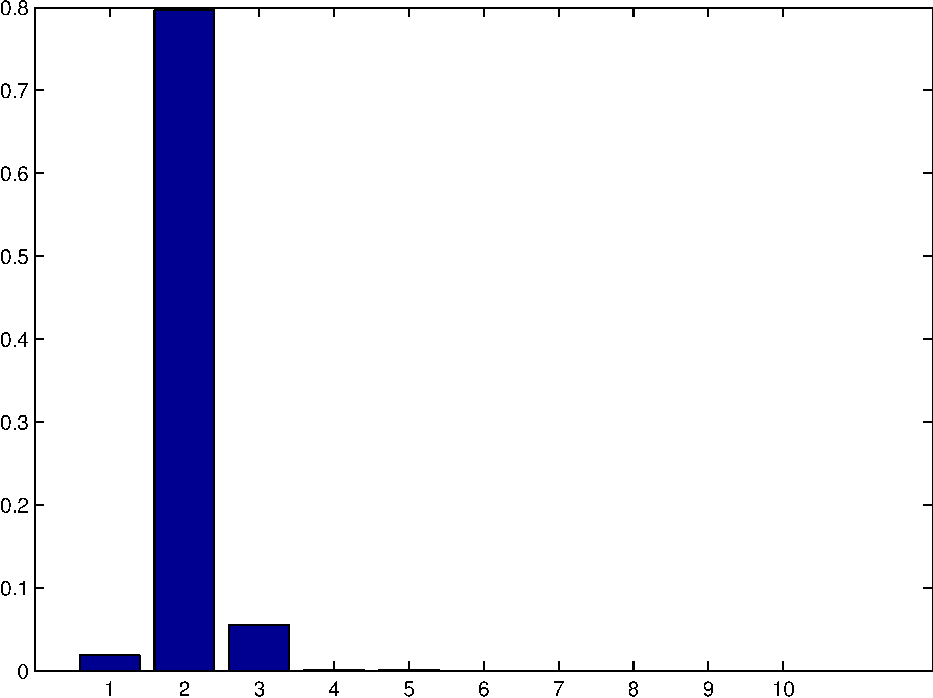
\includegraphics[width=50mm,height=42.5mm]
{../diagrams/demOilVargplvmLengthScales1}&
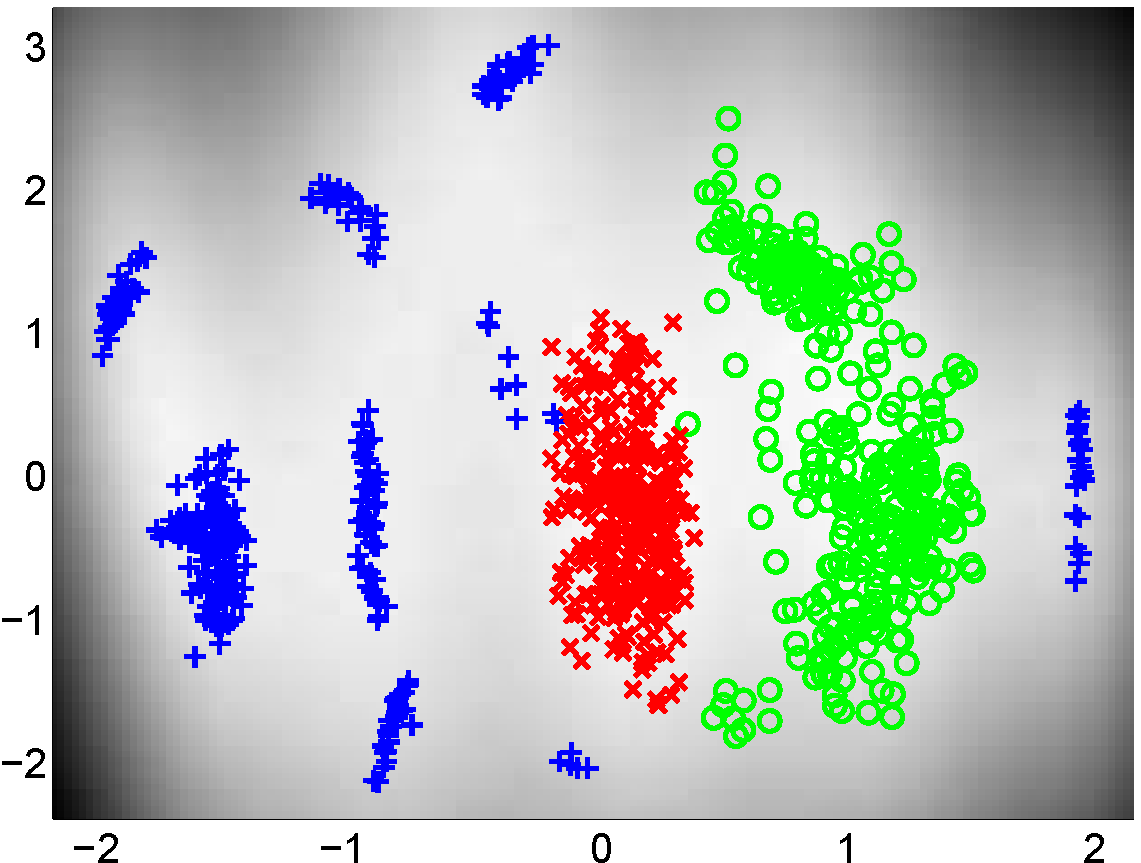
\includegraphics[width=50mm,height=42.5mm]
{../diagrams/demOilVargplvm1} &
\includegraphics[width=50mm,height=42.5mm]
{../diagrams/demOilFgplvm7.eps}\\
(a) & (b) & (c)
\end{tabular}
\caption{Panel (a) shows the inverse lengthscales found by applying the
  Bayesian GP-LVM with ARD SE kernel on the oil flow data. Panel (b)
  shows the visualization achieved by keeping the most dominant latent
  dimensions (2 and 3) which have the largest inverse lengthscale
  value. Dimension 2 is plotted on the
  $y$-axis and 3 and on the $x$-axis. Plot (c) shows the visualization found
  by standard sparse GP-LVM.
\label{fig:Oil}}
\end{center}
\end{figure*}

\vspace{-2mm}
\subsection{Frey Faces Data}
\vspace{-2mm}



\begin{figure*}[ht]
\begin{center}
\begin{tabular}{cccccccc}
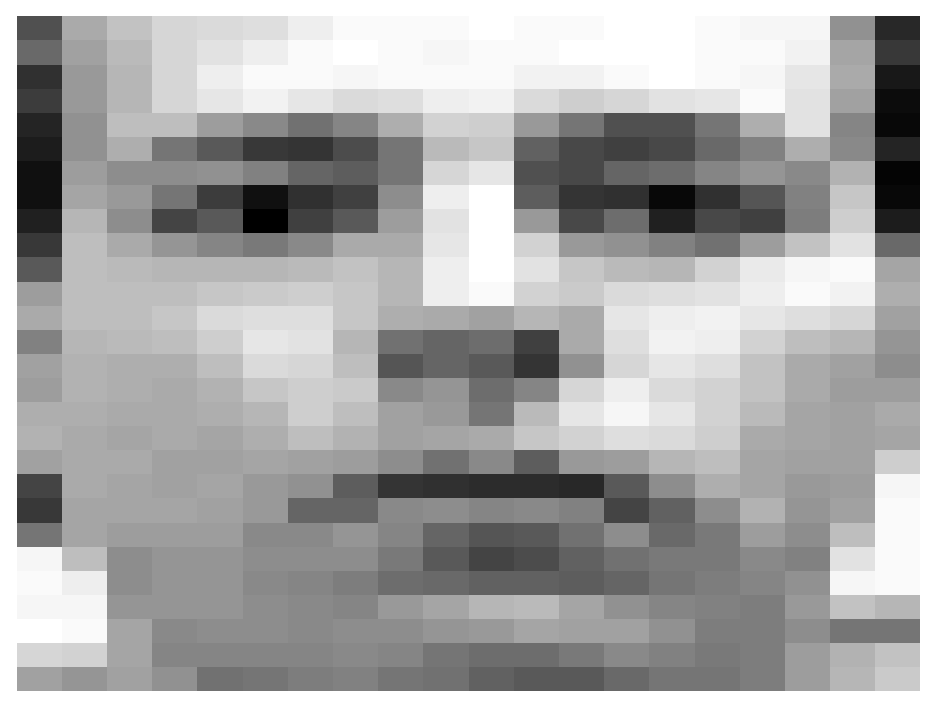
\includegraphics[width=16mm,height=13mm]
{../diagrams/demBrendanTestImag1_3.eps}&
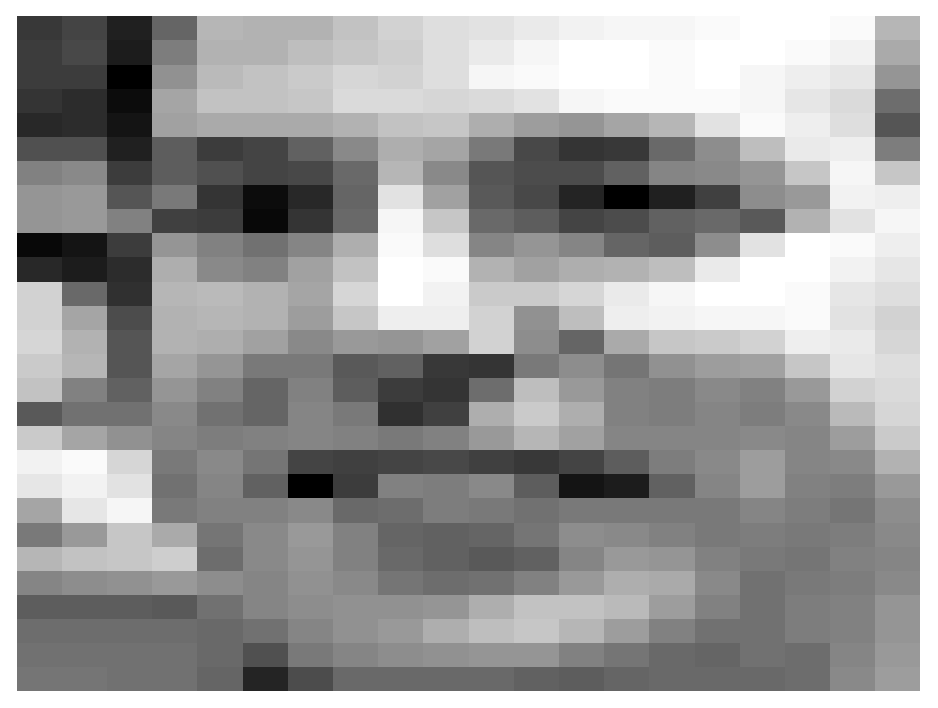
\includegraphics[width=16mm,height=13mm]
{../diagrams/demBrendanTestImag2_3.eps} &
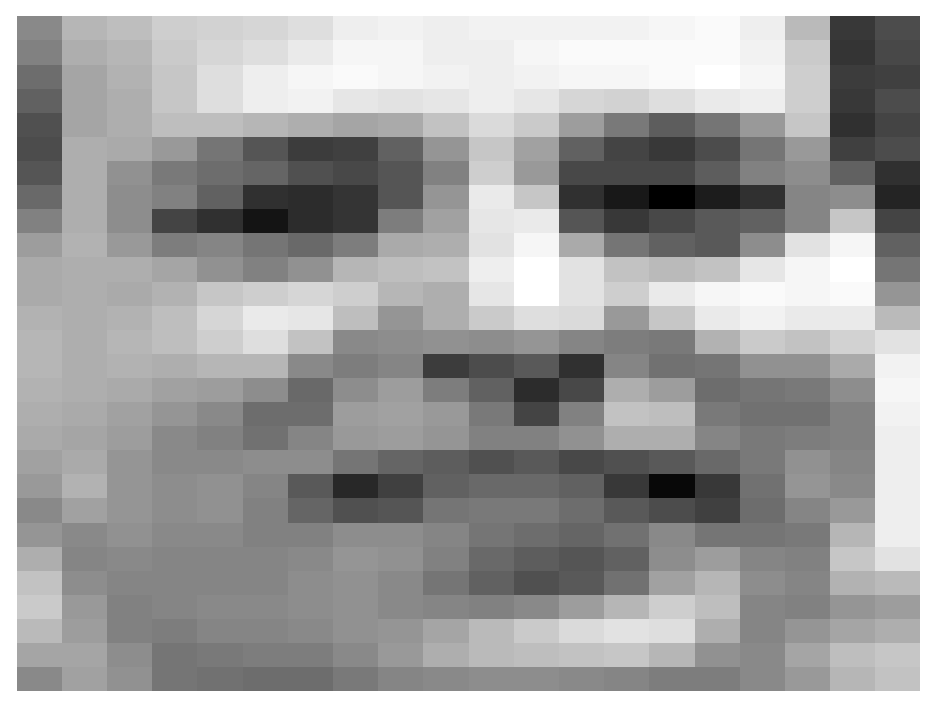
\includegraphics[width=16mm,height=13mm]
{../diagrams/demBrendanTestImag4_3.eps}&
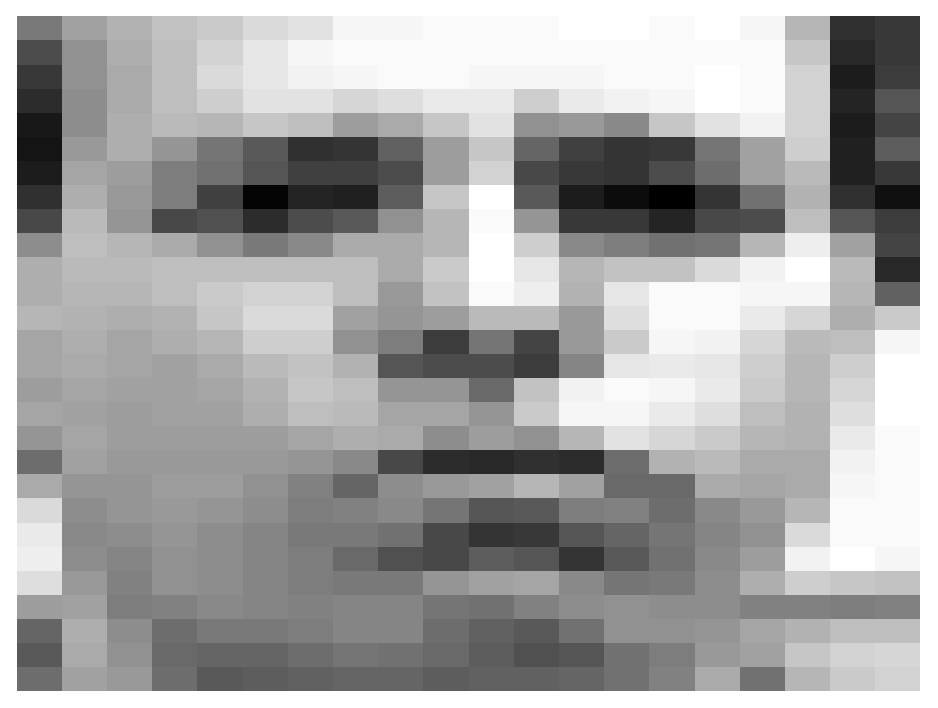
\includegraphics[width=16mm,height=13mm]
{../diagrams/demBrendanTestImag11_3.eps}&
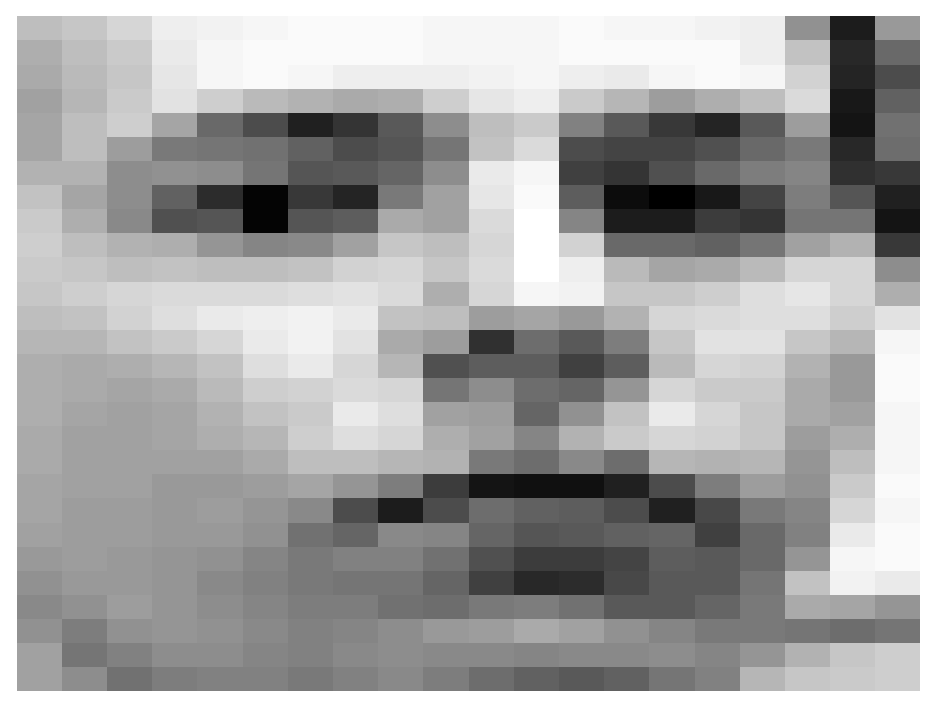
\includegraphics[width=16mm,height=13mm]
{../diagrams/demBrendanTestImag24_3.eps}&
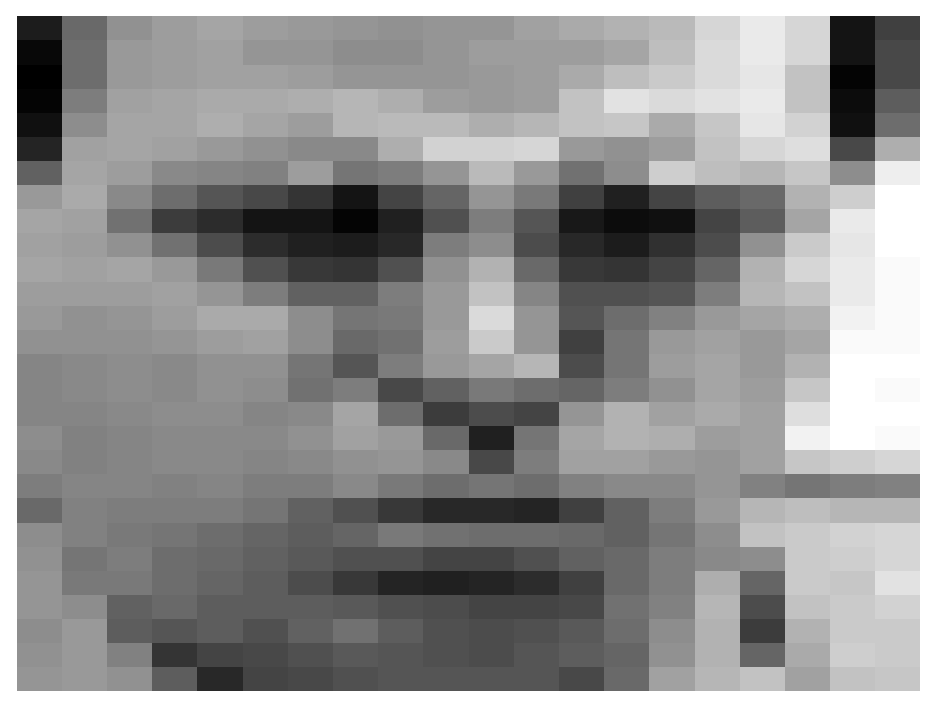
\includegraphics[width=16mm,height=13mm]
{../diagrams/demBrendanTestImag51_3.eps}&
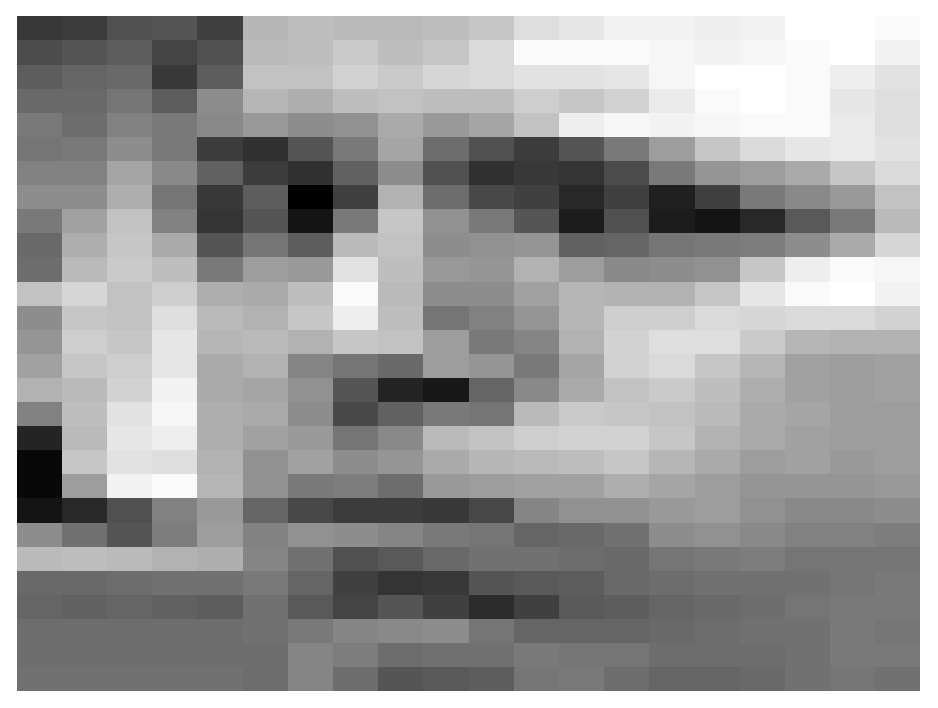
\includegraphics[width=16mm,height=13mm]
{../diagrams/demBrendanTestImag62_3.eps}&
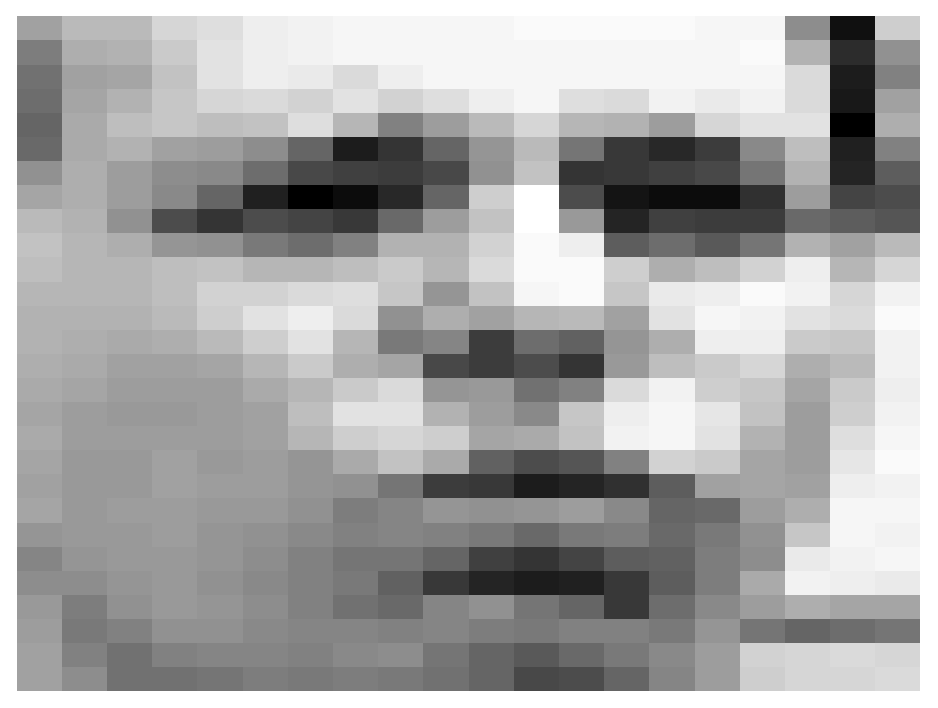
\includegraphics[width=16mm,height=13mm]
{../diagrams/demBrendanTestImag127_3.eps}\\
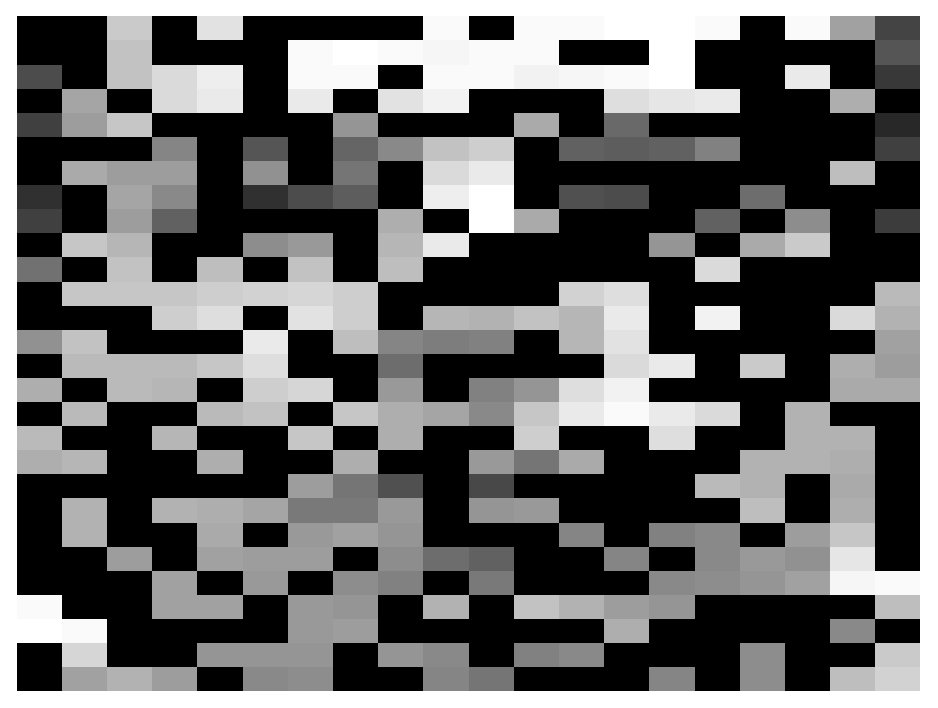
\includegraphics[width=16mm,height=13mm]
{../diagrams/demBrendanTestImag1WithMissing_3.eps}&
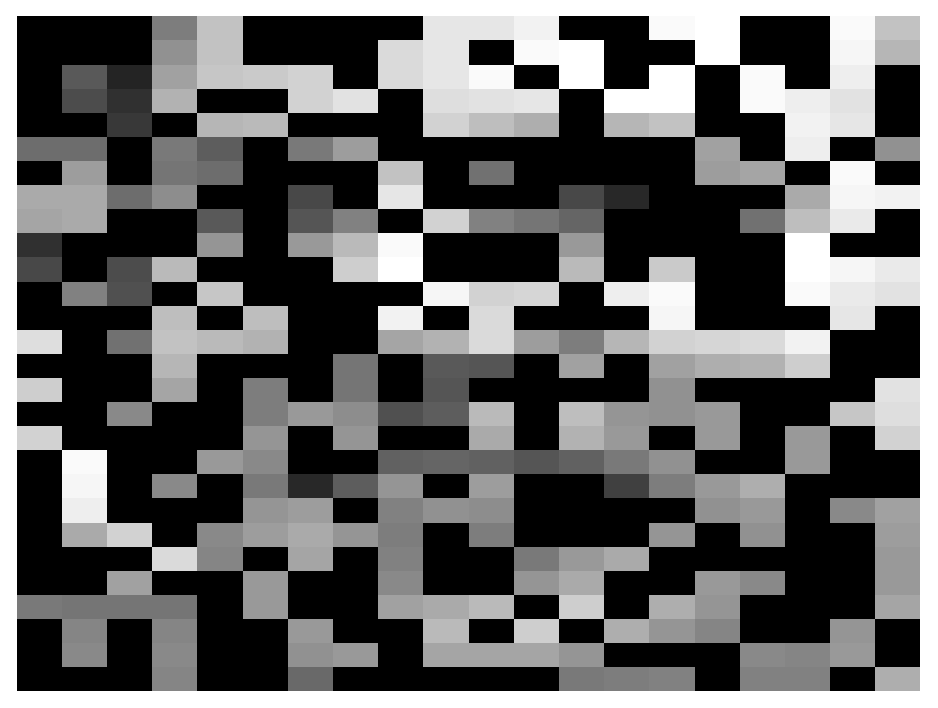
\includegraphics[width=16mm,height=13mm]
{../diagrams/demBrendanTestImag2WithMissing_3.eps} &
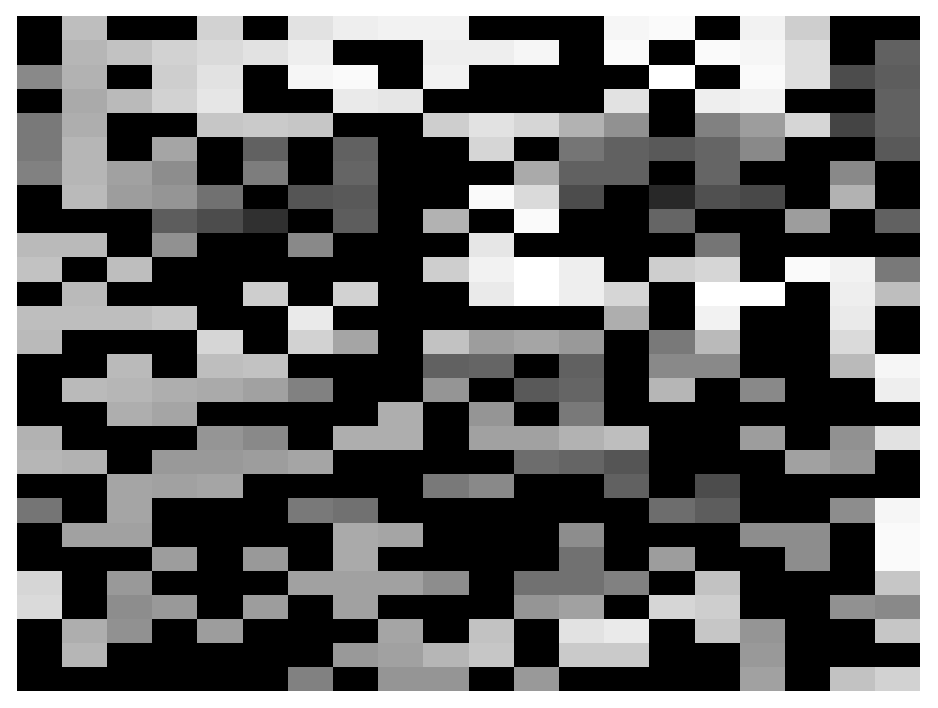
\includegraphics[width=16mm,height=13mm]
{../diagrams/demBrendanTestImag4WithMissing_3.eps}&
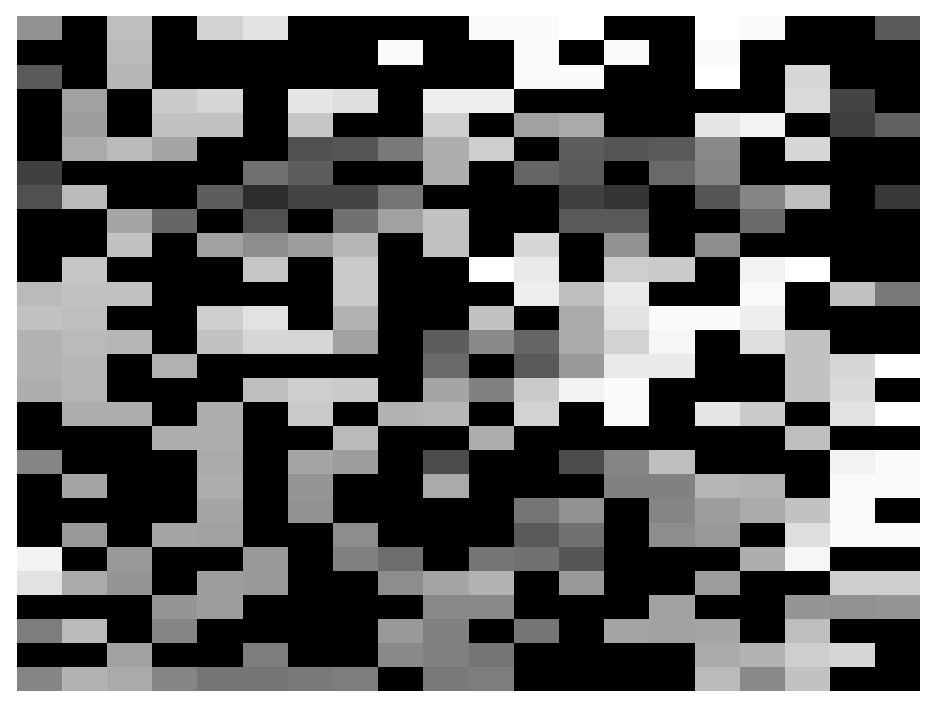
\includegraphics[width=16mm,height=13mm]
{../diagrams/demBrendanTestImag11WithMissing_3.eps}&
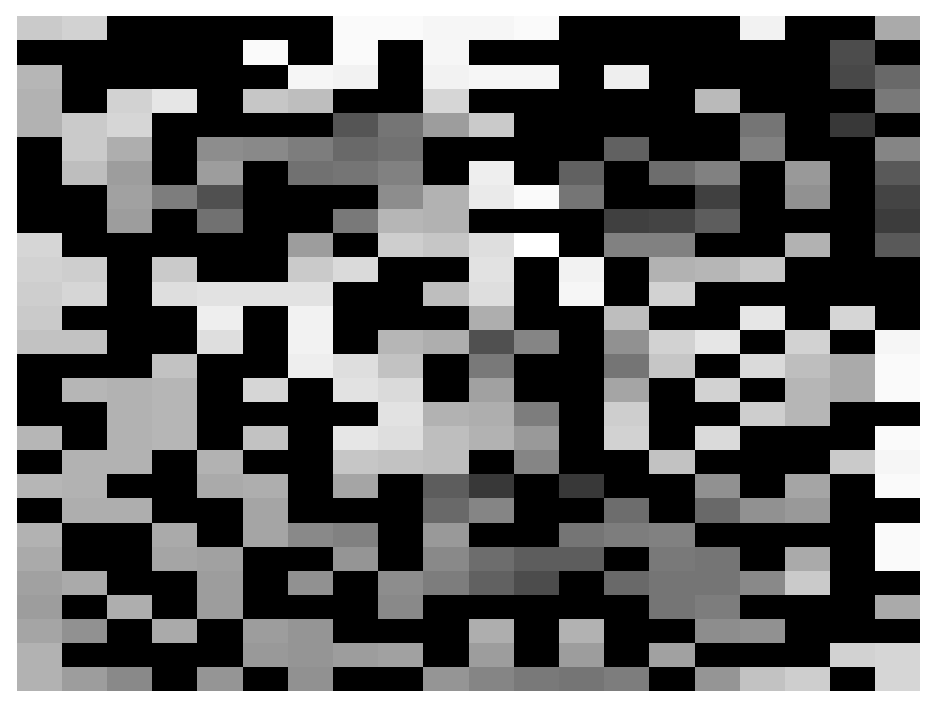
\includegraphics[width=16mm,height=13mm]
{../diagrams/demBrendanTestImag24WithMissing_3.eps}&
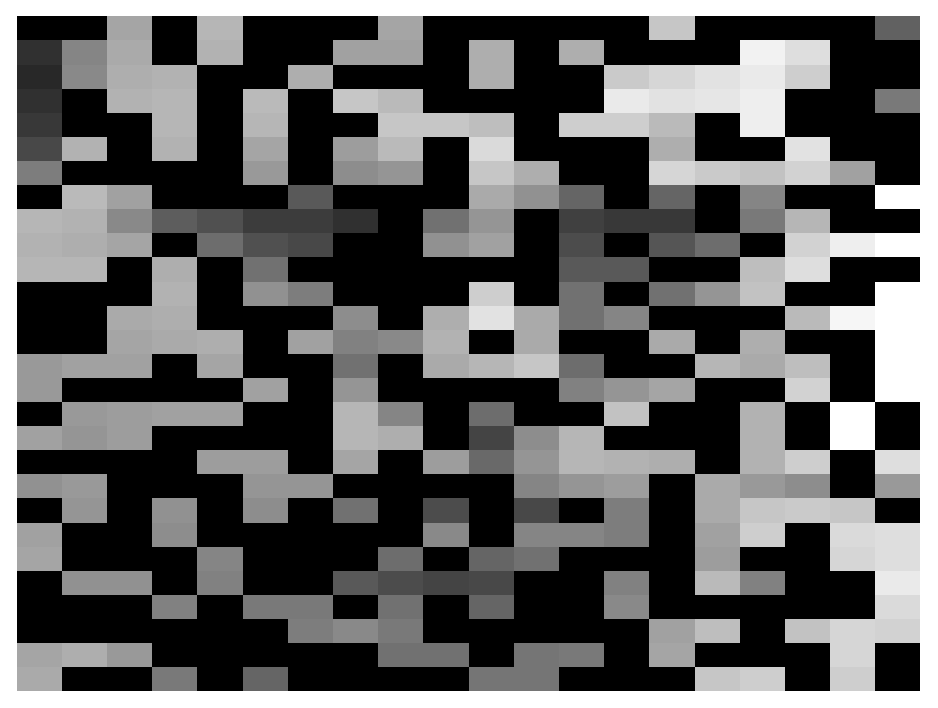
\includegraphics[width=16mm,height=13mm]
{../diagrams/demBrendanTestImag51WithMissing_3.eps}&
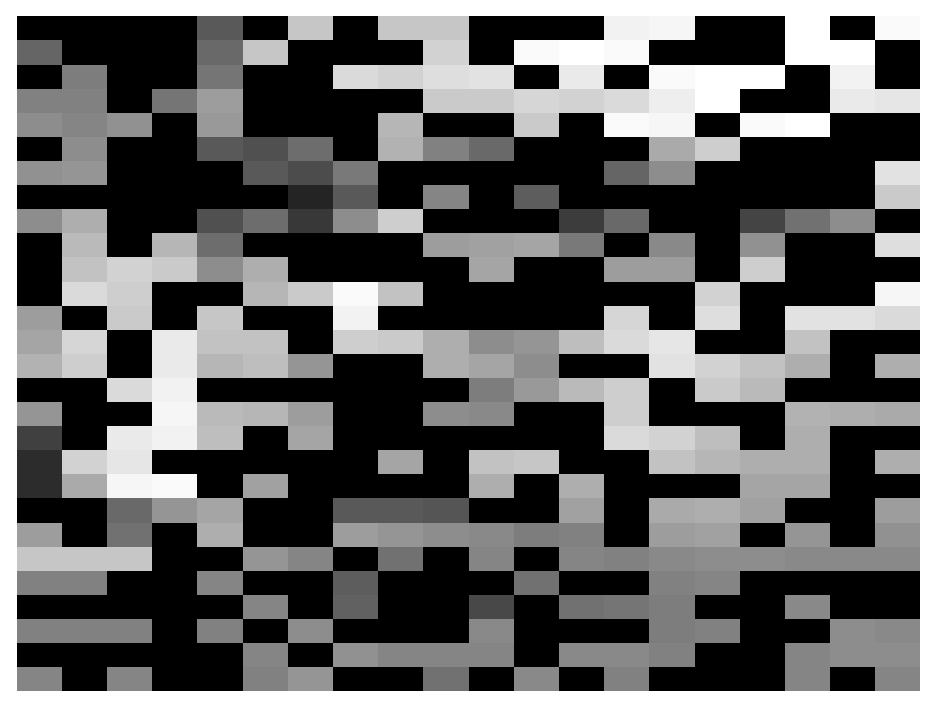
\includegraphics[width=16mm,height=13mm]
{../diagrams/demBrendanTestImag62WithMissing_3.eps}&
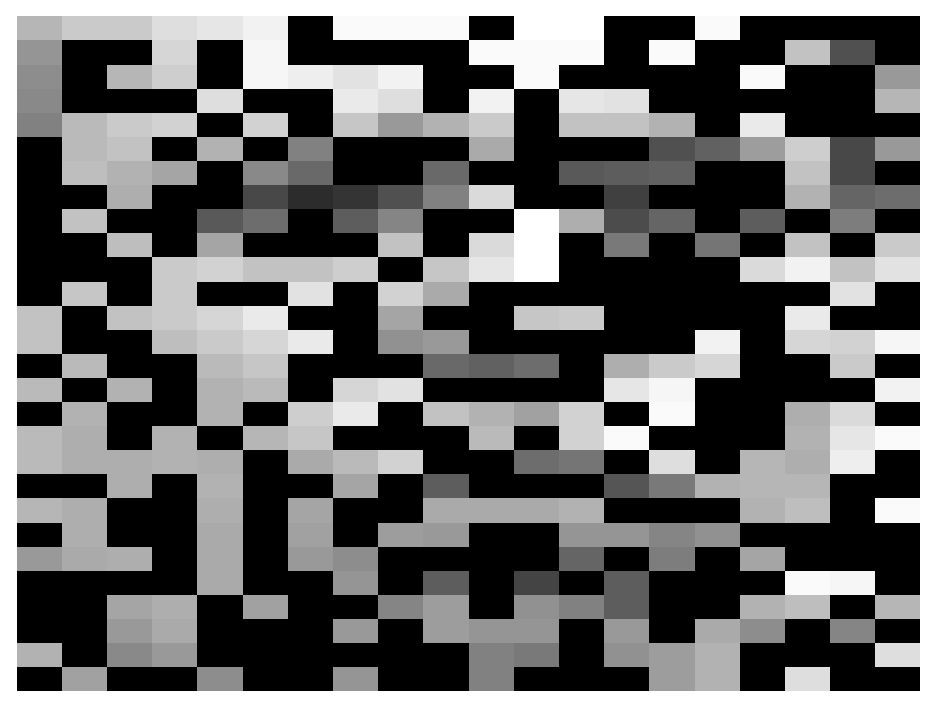
\includegraphics[width=16mm,height=13mm]
{../diagrams/demBrendanTestImag127WithMissing_3.eps}\\
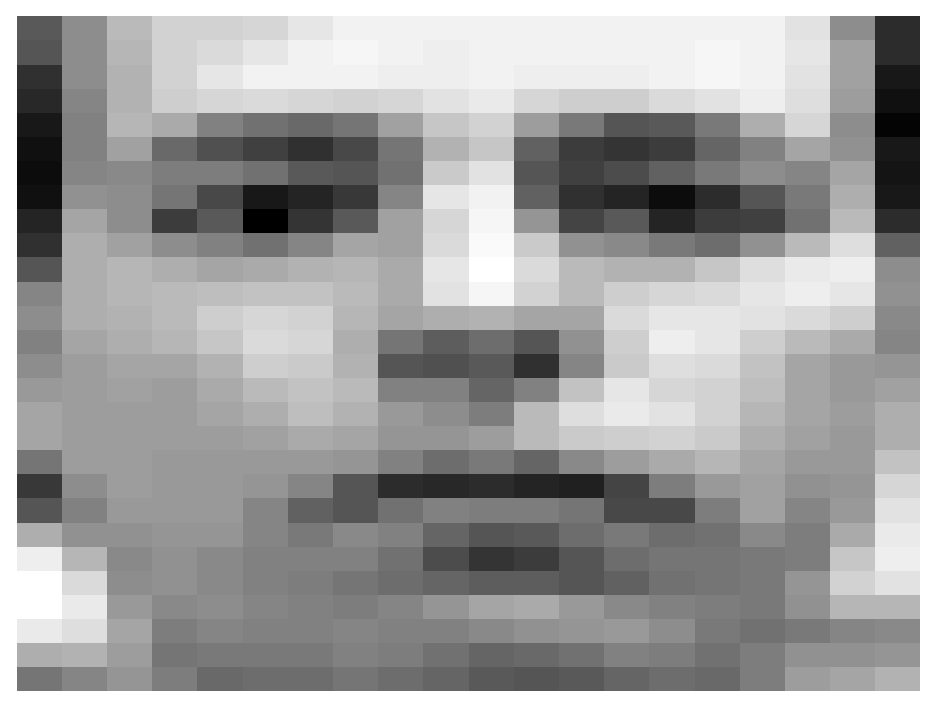
\includegraphics[width=16mm,height=13mm]
{../diagrams/demBrendanTestImag1Reconst_3.eps}&
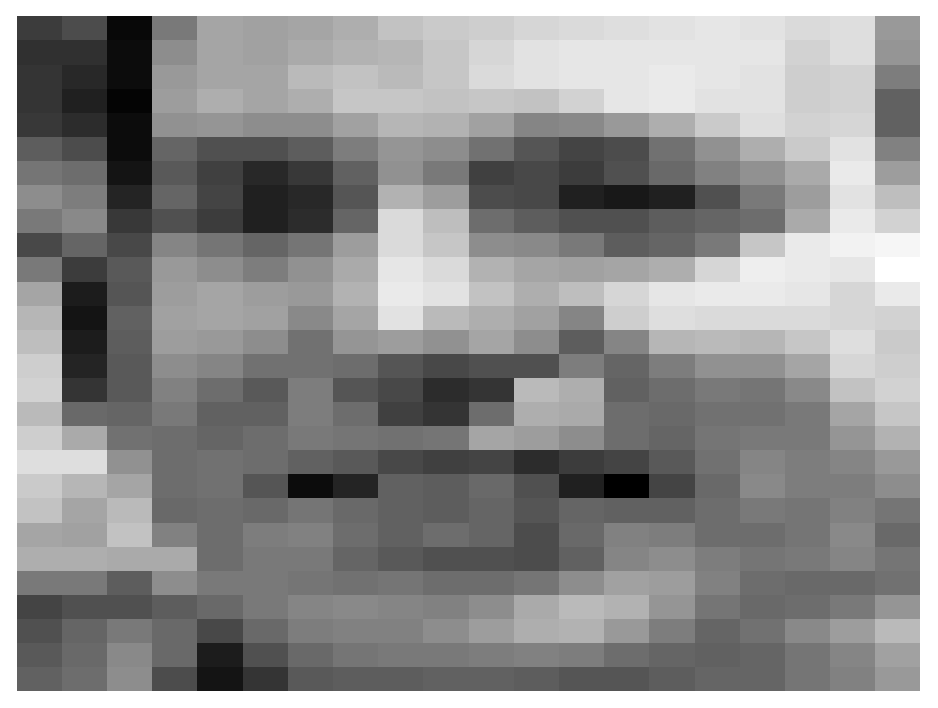
\includegraphics[width=16mm,height=13mm]
{../diagrams/demBrendanTestImag2Reconst_3.eps} &
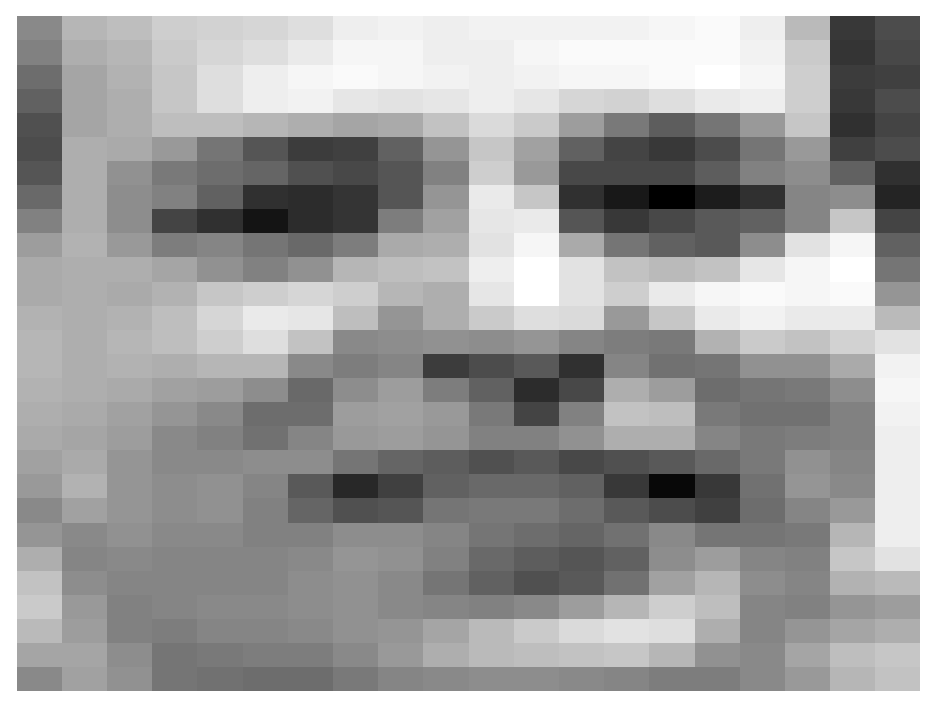
\includegraphics[width=16mm,height=13mm]
{../diagrams/demBrendanTestImag4Reconst_3.eps}&
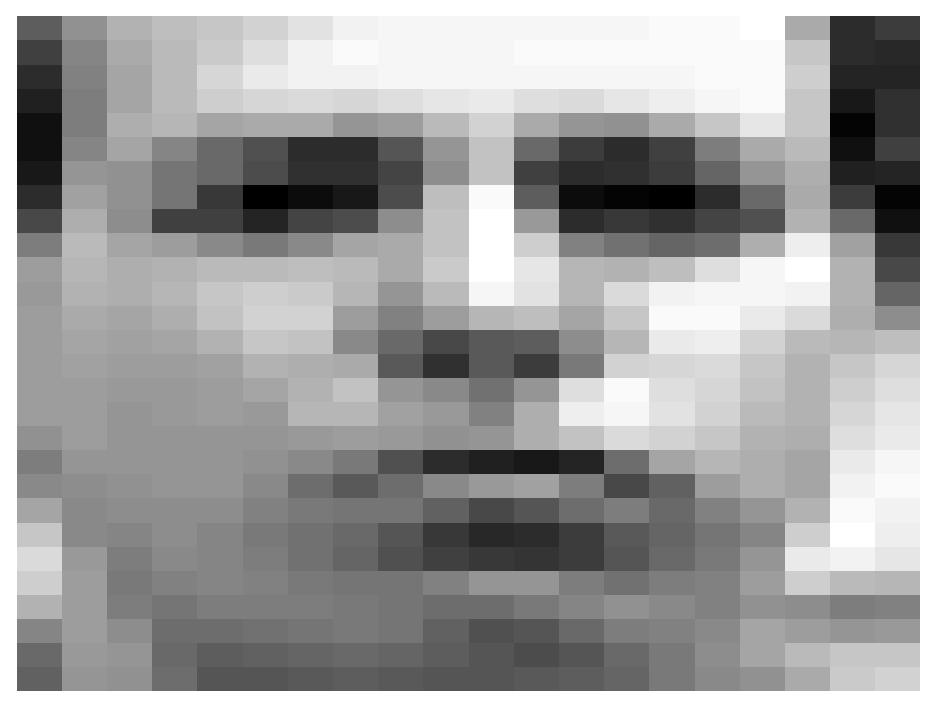
\includegraphics[width=16mm,height=13mm]
{../diagrams/demBrendanTestImag11Reconst_3.eps}&
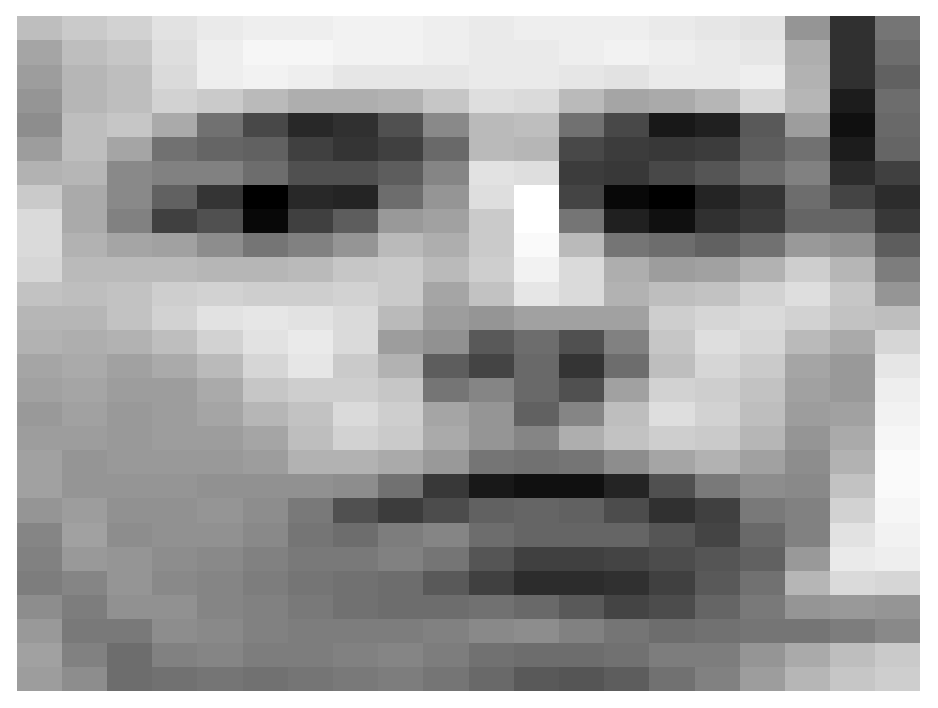
\includegraphics[width=16mm,height=13mm]
{../diagrams/demBrendanTestImag24Reconst_3.eps}&
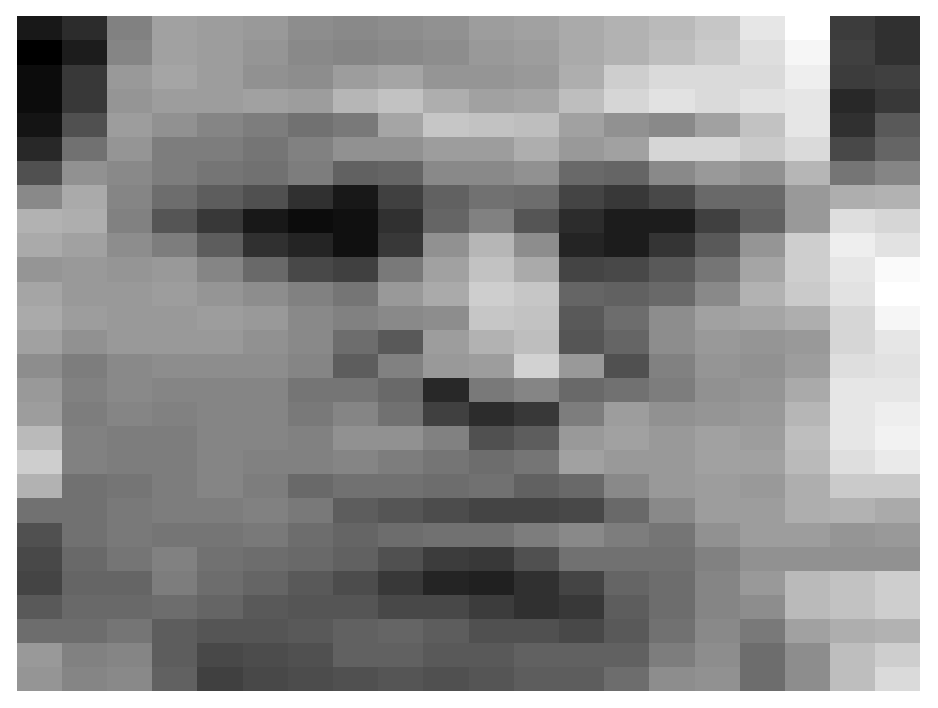
\includegraphics[width=16mm,height=13mm]
{../diagrams/demBrendanTestImag51Reconst_3.eps}&
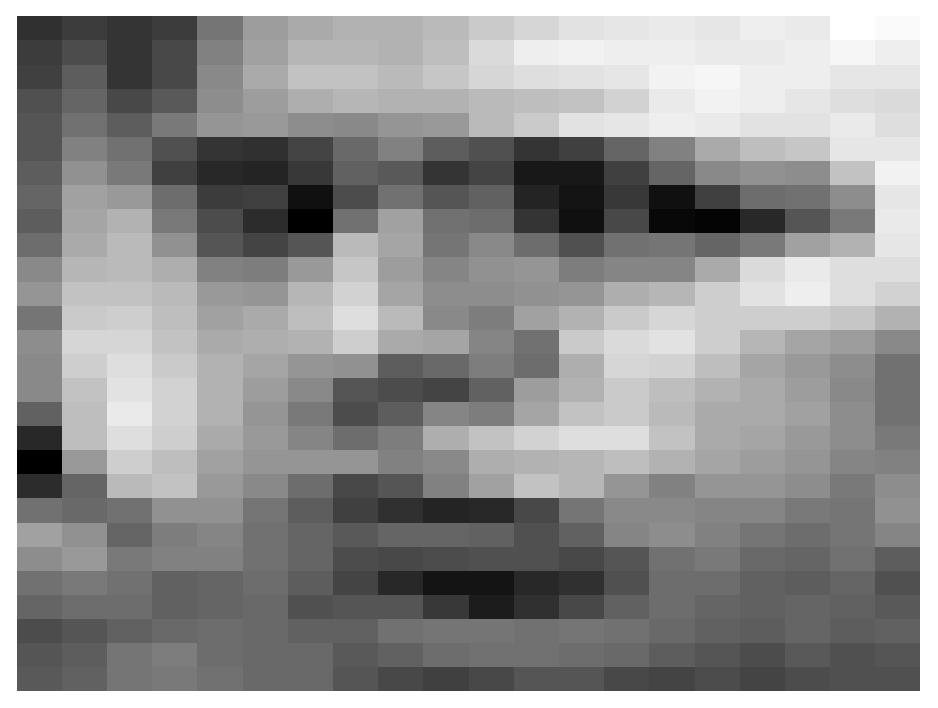
\includegraphics[width=16mm,height=13mm]
{../diagrams/demBrendanTestImag62Reconst_3.eps}&
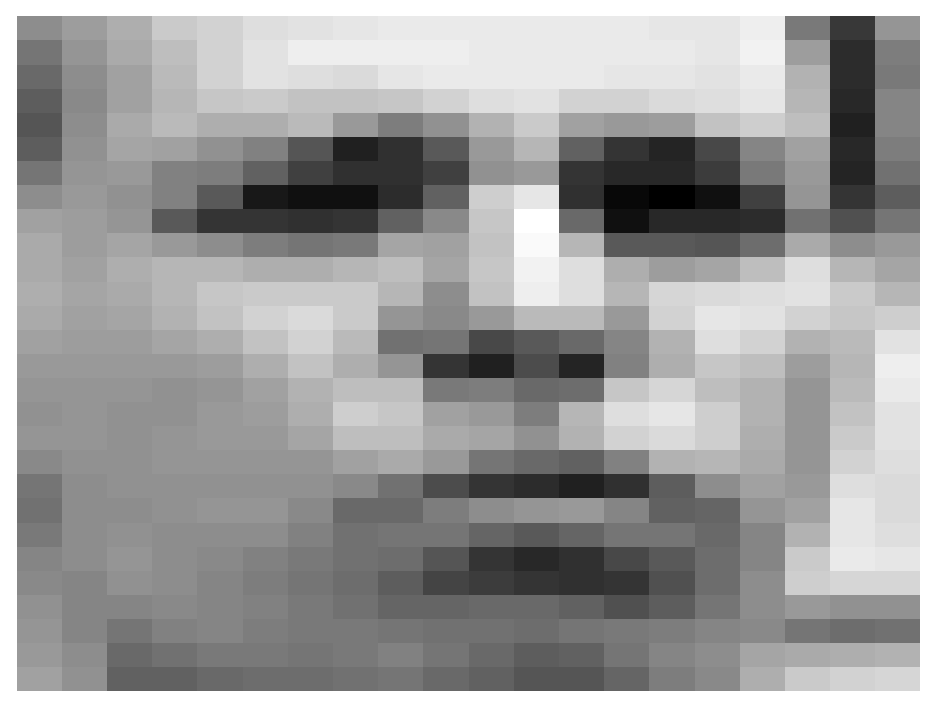
\includegraphics[width=16mm,height=13mm]
{../diagrams/demBrendanTestImag127Reconst_3.eps}
\end{tabular}
\caption{Examples of reconstruction of partially observed test images 
in Frey faces by applying the Bayesian GP-LVM. Each column corresponds to a test
image. In every column, the top panel shows the true test image, 
the middle panel the partially observed image (where missing pixels are
shown in black) and the bottom image is the reconstructed image. 
\label{fig:BrendanFaces}}
\end{center}
\end{figure*}



Here, we consider a dataset of faces \citep{Roweis:global01} taken
from a video sequence that consists of $1965$ images of size $28
\times 20$. In this dataset, we would like to exploit the ability of
the model to reconstruct partially observed test data. Therefore, we
train the model using a random selection of $1000$ images and then we
consider the remaining $965$ images as test data. Furthermore, in each
test image we assume that only half of the image pixels are
observed. The missing pixels were chosen randomly for each test
image. After training on $1000$ images, each partially observed test
image was processed separately (this involves the optimization of the
corresponding variational distribution as discussed in section
\ref{sec:predictiontest}) and the missing pixels were
predicted. Figure \ref{fig:BrendanFaces} shows a few examples of
reconstructed test images.  Each column in this figure corresponds to
a test image, where the top plot shows the true test image, the middle
one the partially observed image and the bottom image shows the
reconstructed image.  We also measure the mean absolute reconstruction
error over all test images and missing pixels and compare this error
with the standard sparse GP-LVM. This standard GP-LVM was applied
using several settings of the latent dimensionality: $Q=2,5,10$ and
$30$. The Bayesian GP-LVM was trained once using $30$ latent
dimensions. The latent variables $X$ in the standard GP-LVM and the
means of the variational distribution in Bayesian GP-LVM were
initialized through PCA.  The error for Bayesian GP-LVM was
$7.4003$. For the standard GP-LVM the error was $10.5748$, $9.7284$,
$19.6949$ and $19.6961$ for $2, 5, 10$ and $30$ latent dimensions
respectively. Notice that the standard GP-LVM has poor performance for
large value of latent dimension and achieves the best error when we
consider $5$ latent dimensions. Nevertheless, this was still worse
than the error from the Bayesian GP-LVM. Finally, Figure
\ref{fig:BrendanInverseLenghScale} shows the values of the
inverse lengthscales obtained by the maximization of the variational
lower bound. Although, in this case, the algorithm does not shrink
some of the dimensions completely to zero, it does force many of them
to obtain small values. Note that one of the dimensions (the
first from the left) seems to be the most important in
explaining the data.

\begin{figure}[ht]
\begin{center}
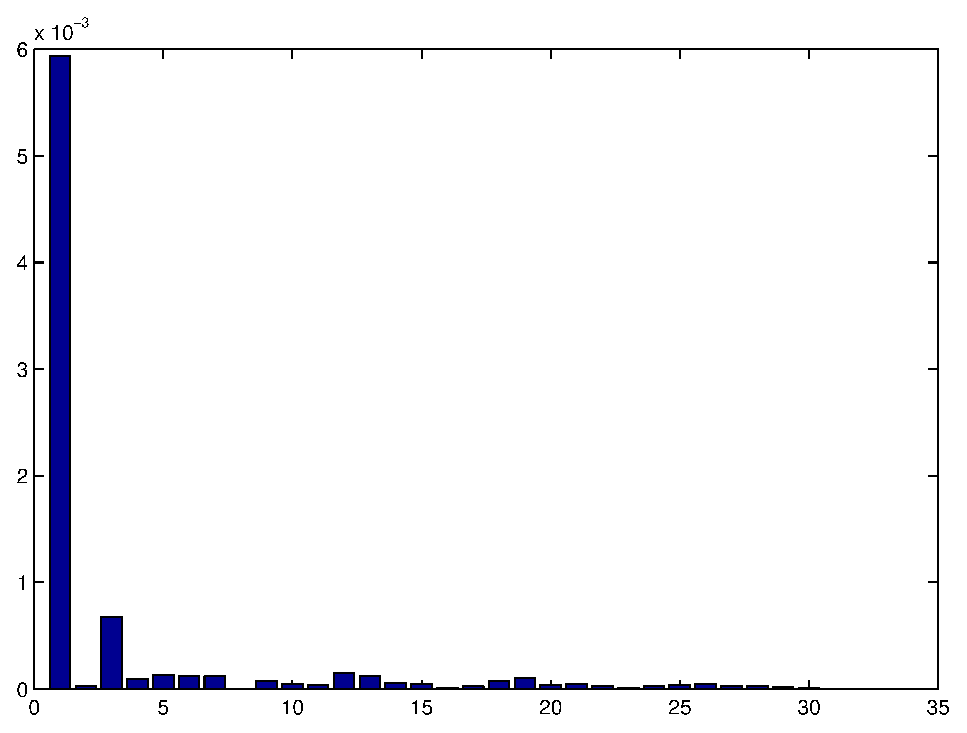
\includegraphics[width=55mm,height=45mm]
{../diagrams/demBrendanVargplvmLengthScales3.eps}
\caption{This plot shows the values of the inverse lengthscales
found by using the Bayesian GP-LVM with ARD SE kernel in Frey faces.  
\label{fig:BrendanInverseLenghScale}}
\end{center}
\end{figure}


\vspace{-6mm}
\subsection{Digits Data}
\vspace{-2mm}

In the final experiment we use the Bayesian GP-LVM to build a
generative classifier for handwritten digit recognition. We consider
the well known USPS digits dataset. This dataset consists of $16
\times 16$ images for all $10$ digits and it is divided into $7291$
training examples and $2007$ test examples.  We run $10$ Bayesian
GP-LVMs, one for each digit, on the USPS data base. We used $10$
latent dimensions and $50$ inducing variables for each model. This
allowed us to build a probabilistic generative model for each digit so
that we can compute Bayesian class conditional densities in the test
data having the form $p(\bfy_*|Y,\text{digit})$. These class
conditional densities are approximated through the ratio of lower
bounds in eq.\ (\ref{eq:ApproxpredictedDensity}) as described in
section \ref{sec:predictiontest}.  The whole approach allows us to
classify new digits by determining the class labels for test data
based on the highest class conditional density value and using a
uniform prior over class labels.  The test error made by the Bayesian
GP-LVM in the whole set of $2007$ test points was $95$ incorrectly
classified digits i.e.\ 4.73\% error. 
% This is comparable to many
%advanced discriminative classifiers that have been applied in this
%problem.

%A confusion matrix is given in Table ??. 

\vspace{-2mm}
\section{Discussion}
\vspace{-3mm}

We have introduced an approximation to the marginal likelihood of the
fully marginalized Gaussian process latent variable model. Our
approximation is in the form of a variational lower bound. With the
fully marginalized model we can automatically determine the latent
dimensionality of a given data set. We demonstrated the utility of
this rigorous lower bound on a range of disparate real world data
sets.

Our approach can immediately be applied to training Gaussian processes
with uncertain inputs where these inputs have Gaussian prior
densities. We also envisage several other extensions that
become computationally feasible using the same set of methodologies we
espouse. Dynamical models based on the GP-LVM have been proposed. It
would be straightforward to include a latent space prior with a
temporal component. This could be a Kalman filter, a general Gaussian
process \citep{Lawrence:hgplvm07} or an auto regressive Gaussian
process \citep{Wang:gpdm05}. By using our approach to propagating the
Gaussian noise through the dynamics and the latent space a variational
lower bound on the likelihood of these models could be derived. The
importance of such nonlinear models is clear from the success of
unscented Kalman filters and the related ensemble Kalman filter.

The optimization procedure has a similar computational cost to that of
previously proposed sparse GP-LVMs. We believe there is scope to
improve the speed of the optimization procedure by better exploiting
the correlation present in the parameters. A potential strategy would
be to use the control points idea used to speed up MCMC in GPs 
\citep{Titsias:efficient08} in order to encode the 
variational posterior, effectively decoupling these correlations and
speeding convergence of the optimizer.

\subsubsection*{Acknowledgements}
\vspace{-2mm}
We wish to thank Mauricio \'Alvarez for his help with the software implementation.
This work is funded by EPSRC Grant No EP/F005687/1
"Gaussian Processes for Systems Identification with
Applications in Systems Biology".

\small{
\bibliographystyle{abbrvnat}
\bibliography{lawrence,other,zbooks}
}



\end{document}


%---------------------------------------------- PREDICTIONS ---------------------------------------------------------------------
\section{Predictions with the Variational GP-LVM \label{section:predictions}} 

In this section we explain how the proposed Bayesian models
can accomplish various kinds of predictive tasks.
Firstly, we focus on the Bayesian equivalent of the standard GP-LVM model
(\ie when a standard normal prior is employed for the latent space) and
then we consider the dynamical version of the model.
The first kind of inference discussed here concerns calculating the probability density
probability density $p(Y_* | Y)$ of some observed test data
$Y_* \in \mathbbm{R}^D $, which is allowed to have missing
values. The computation of this probability can allow us to use the
model as a density estimator which, for instance, can represent the
class conditional distribution in a generative based classification
system.  We will exploit such a use in section \ref{sec:experiments}.
Secondly we discuss how we can probabilistically reconstruct 
 partially observed test data  $Y_*^{p} \in \mathbb{R}^{N_* \times D_p}$ from the whole $Y_*
= (Y_*^{p}, Y_*^{m})$, where $p$ and $m$ are set indices indicating
the present (\ie observed) and missing dimensions of $Y_*$
respectively, so that $p \cup m= \{1,\ldots,D\}$.
The missing dimensions are reconstructed by computing the
Bayesian predictive distribution $p(Y_*^{m}| Y_*^{p}, Y)$.
This second prediction task can also be used to 
remove the noise of a fully observed output. 
If the test points are known to form timeseries, then the aforementioned predictive
tasks can be solved with the dynamical version of our model.
In this case, the test points $Y_*$ are accompanied by their
corresponding timestamps $\bft_*$. Further, the dynamical model also enables performing
extrapolation, \ie computing novel outputs given only a test time vector $\bft_*$.
The inference procedures for the dynamical model are discussed in section \ref{predictionsDynamical}.

%In the case where $Y_*$ constitutes a multivariate timeseries,
%it is additionally associated with with the corresponding timestamps
%$\bft_* \in \mathbb{R}^{N_*}$.

\subsection{Predictions with the standard Variational GP-LVM}

\subsubsection{\label{predictions1} Calculating the density $p(Y_*|Y)$}
By introducing the latent variables $X$ (corresponding to the
training outputs $Y$) and the new test latent variables 
$X_* \in \mathbb{R}^{N_* \times Q}$, the
previous density of interest as the ratio of two marginal likelihoods:

\begin{equation}
\label{pyystar1}
p(Y_*|Y) = \frac{p(Y_*,Y)}{p(Y)} = 
	\frac{\int p(Y_*, Y | X, X_*) p(X,X_*) \intd X \intd X_*}{\int p(Y|X) p(X) \intd X}
\end{equation}
%
In the denominator 
we have the marginal likelihood of the GP-LVM for which we have already
computed a variational lower bound.  The numerator is another 
marginal likelihood that is obtained by augmenting the training data
$Y$ with the test point $Y_*$ and integrating out both $X$ and the 
newly inserted latent variable $X_*$. To approximate the density 
 $p(Y_* |Y)$, we construct a ratio of lower bounds as follows. 

The quantity $ \int p(Y | X) p(X) d X$ is approximated by the
 lower bound $e^{\F(q(X),Y)}$ where 
$\F(q(X),Y)$ is the variational lower bound as computed in section \ref{}
and is given in equation \eqref{jensensSplit2}. The maximization   
of this lower bound  specifies the variational
distribution $q(X)$ over the latent variables in the training
data. Then, this distribution  remains fixed during test time.     
$\int p(Y_*,Y | X, X_*) p(X,X_*) d X d X_*$ 
is approximated by the lower bound $e^{\F(q(X,X_*), Y_*,Y)}$ which has
exactly analogous form to \eqref{jensensSplit2}. 
This optimisation is fast, because due to the prior used for the standard
GP-LVM, in equation \eqref{standardNormal}, we can write
$q(X,X_*) = q(X) q(X_*)$. Then, $q(X)$ is held fixed during test time and we only need
to optimise with respect to the $2 (N_* \times Q)$ parameters of the variational
Gaussian distribution $q(X_*)=\prod_{n=1}^{N_*} q(\bfx_n) = \prod_{n=1}^{N_*} \mathcal{N}(\bfmu_*,S_{n,*})$ 
(recall that $S_{n,*}$ is a diagonal matrix). 
Further, since the $Psi$ statistics decompose
across data, during test time we can re-use the already estimated $Psi$ statistics
corresponding to the averages over $q(X)$ and only need to compute the extra average
terms associated with $q(X_*)$.
Note that optimization of the parameters $(\bfmu_*,S_{n,*})$ of $q(x_{n,*})$ are subject
to local minima. However, 
sensible initializations of $\bfmu_*$ can be employed based on the 
mean of the variational distributions associated with the nearest
neighbours of each test point $\bfy_{n,*}$ in the training data $Y$. 
%

%Furthermore, such optimization is fast because we can perform  
%several precomputations in advance. In particular, 
%due to the prior used for the standard GP-LVM, in equation \eqref{standardNormal},
%all latent points $\bfx \in \left[ X, X_* \right] $ are uncoupled. Therefore,
%the computation of the
%$\Psi$ statistics decomposes across data and updating 
%these statistics  to account for the 
%insertion of $N_*$ test points, involves only averages over the $N_*-dimensional$ 
%variational distribution $q(X_*)$.
%
Finally, the approximation 
of $p(Y_* |Y)$ is given by 
\begin{equation}
p(Y_* |Y) = e^{ \F(q(X,X_*),Y,Y_*) - \F(q(X),Y)  }. 
\label{eq:predictive1}
\end{equation}





%
%
%Notice that the denominator constitutes the marginal
% likelihood of the training data (equation \eqref{marginalLikelihood}) for
%the logarithm of which we have already computed the variational lower bound 
%$\mathcal{F} = \mathcal{F}(q(X))$ of equation \eqref{jensensSplit} during training.
%
%
%As for the numerator of equation \eqref{pyystar1}, its logarithm can be approximated by a variational lower bound
%$\mathcal{F}^* = \mathcal{F} (q(X,X_*))$, which has exactly analogous form to \eqref{marginalLikelihood}. Indeed,
%this quantity bounds the logarithm of the marginal likelihood of the training data augmented with the test ones, where
%both $X$ and the newly inserted latent variables $X_*$ need to be integrated out. 
%Therefore, this bound will now be a function of a variational distribution $q(X,X_*)$
%which needs to be optimised so that its marginal $q(X_*)$ approximates the true posterior $p(X_* | Y_*,Y)$.
%After this procedure, we will be able to
%replace the numerator of \eqref{pyystar1} with $e^{\mathcal{F} (q(X,X_*))}$ and the denominator with $e^{\mathcal{F} (q(X))}$,
%which is treated as a constant in the test phase. We will then be able to approximate the quantity of interest with the equation
%\begin{equation}
%\label{pyystar2}
%p(Y_*|Y) \approx q(Y_*|Y) = e^{\mathcal{F} (q(X,X_*)) - \mathcal{F} (q(X))}.
%\end{equation}
%
%\noindent What now remains is to define the variational distribution 
%\begin{equation}
%\label{qxxstar}
%q(X,X_*) = q(X) q(X_*|X) .
%\end{equation}
%At this step, the inference procedure
%differs depending on the type of prior used for the latent space $X$. The prior \eqref{qXstatic} leaves all the latent points
%uncoupled, whereas the dynamical prior \eqref{priorXgivenT} couples the test latent points $\bfx_{n,*}$ with each other as well as with the
%training latent points stored in $X$. In the first case, equation \eqref{qxxstar} can be written as 
%$q(X,X_*) = \prod_{n=1}^N q(\bfx_n) \prod_{n=1}^{N_*} q(\bfx_{n,*})$, 
%where $q(\bfx_{n,*}) = \mathcal{N}(\bfx_{n,*} | \bfmu_{n,*}, S_{n,*})$. 
% This means that we only need to optimise with respect to the $2 (N_* \times Q)$ parameters of $q(X_*)$ 
% (recall that $S_{n,*}$ is a diagonal matrix). 
% The rest of the parameters
%on which the variational bound $\mathcal{F}(q(X,X_*))$ depend, are held fixed to the values learned during training.
%We can perform several precomputations to improve efficiency. In particular, notice that the computation
%of the $\Psi$ quantities decomposes across data (as can be seen in the supplementary material and in \cite{BayesianGPLVM})
%% \highlight{TODO:(equations for Psis)} 
%and therefore, 
%%because they only appear in the  ..... . Therefore,
%updating
%these statistics to account for the insertion of the test point
%involves only averages over the factorised variational distribution $q(X_*)$.
%
%\par On the other hand, performing inference in the dynamical model is more challenging, since $q(X,X_*)$ is fully
%coupled across $X$ and $X_*$. Therefore, if we wish to maintain the correlation of the inputs depending on their times,
%we should select this distribution to only factorise across features: 
%$q(X,X_*) = \prod_{q=1}^Q  \mathcal{N} (\bfx_{q,*} | \bfmu_{q,*} ,S_{q,*})$,
% where $S_{q,n}$ are full $(N+N_*) \times (N+N_*)$ matrices which can, however, be reparametrised with $N+N_*$
%parameters as discussed in section \ref{optimisation}.
%Consequently, the already learned parameters of $q(X)$ cannot be reused. Instead, we must optimise over the whole set of
%the $2 \left( Q \times (N + N_*) \right)$ parameters involved in $q(X,X_*)$. A much faster but less
%accurate method would be to decouple the test from the training latent variables by imposing the factorisation
%$q(X,X_*) = q(X)q(X_*)$, thus assuming that all training and test points are correlated with points only within their own set.
%This is not used, however, in our current implementation.

%The variational optimisation will now seek
%to optimise the parameters $\bfmu_{q,*}, S_{q,*}$



%---------------------------------------------- PREDICTIONS given partially observed otuputs -------------------------------------
\subsubsection{\label{predictions2} Predictions Given Partially Observed Outputs}

We now discuss the second prediction problem where a set of partially 
observed test points $Y_* = (Y_*^p,Y_*^m)$ are given and 
we wish to reconstruct the missing part $Y_*^m$.
To approximate the predictive density 
we will need to introduce the underlying latent function
values $F_* \in \mathbb{R}^{N_* \times D}$ (the noisy-free version of $Y_*$)
and the latent variables $X_*$. We can then write the predictive density as

\todo{maybe should put $p(X_* , X | Y, Y_*^p)$ instead of $p(X_*| Y, Y_*^p) $}

\begin{equation}
\label{eq:predictive2}
p(Y_*^m | Y, Y_*^p) =  \int p(Y_*^m | F_*^m)  p(F_*^m | X_*, Y, Y_*^p) p(X_*| Y, Y_*^p) \intd  F_*^m \intd  X_* .
\end{equation}
The term $p(F_*^m | X_*, Y, Y_*^p)$ is found by marginalising out the latent function values
corresponding to the inducing points $\tilde{X}$ in the augmented probability model. Therefore,
this term is approximated by the variational distribution
\begin{eqnarray}
\label{eq:qFstarXstar}
q(F_*^m |X_*) & = & \int \prod_{d \in D} p(\bff_{*,d}^m | \bfu_d, X_*)  q(\bfu_d) d \bfu_d 
	    = \prod_{d \in D} q(\bff_{*,d}^m | X_*)  ,
\end{eqnarray}
where $q(\bff_{*,d}^m | X_*)$ is a Gaussian that can be computed analytically,
since in our variational framework the optimal setting for $q(\bfu_d)$ is also found 
to be a Gaussian (eq. \eqref{}).
Specifically, $q(\bff_{*,d}^m | X_*)$
is a factorized Gaussian distribution
where each factor takes the form of the projected process predictive 
distribution \citep{Csato:sparse02,Seeger:fast03,Rasmussen:book06}.
As for the term $p(X_*| Y, Y_*^p)$ of eq. (\ref{eq:predictive2}), it constitutes a
posterior distribution and, thus, can be approximated by a Gaussian variational distribution $q(X,X_*)$.
Following the discussion in section \ref{sec:boundSummary}, we can obtain $q(X,X_*)$
by maximising the variational lower bound on the marginal likelihood:
\begin{align}
p(Y_*^p, Y) ={}&  \int p(Y_*^p, Y|X_*, X) p(X_*, X) \intd  X_* \intd  X \nonumber \\
={}&  \int p(Y^m | X) p(Y_*^p, Y^p|X_*, X) p(X_*, X) \intd  X_* \intd  X.  \label{eq:marginalPredictions2}
\end{align}
We follow the same strategy as in section \ref{predictions1} and approximate the above
quantity with a variational bound. However, now we also have to take into account the information
in $Y_*^p$. Therefore, the marginal likelihood \eqref{eq:marginalPredictions2} is bounded by:
\begin{equation}
\label{eq:predictiveMissing1a}
p(Y_*^p, Y) \geq \int q(X_*, X) \log \frac{ p(Y^m | X) 
    p(Y_*^p, Y^p|X_*, X) p(X_*,X)}{ q(X_*, X)} \intd  X_* \intd  X 
\end{equation}
Since the distributions $q(X,X_*)$ and $p(X,X_*)$ are fully factorised for the standard Variational GP-LVM model,
we can write the above equation as:
\begin{align}
p(Y_*^p, Y) & \geq  \int q(X) \log p(Y^m | X) \intd  X 
    +  \int q(X_*,X) \log p(Y_*^p, Y^p|X_*, X) \intd  X_* \intd  X  \nonumber \\
& - \KL{q(X)}{p(X)} - \KL{q(X_*)}{p(X_*)}. \label{eq:predictiveMissing1b}
\end{align}  
%which has exactly analogous form to the bound \eqref{jensensSplit} computed for the training phase.
Following the discussion in section \ref{sec:boundSummary}, we can rewrite the above bound as
a sum of the following terms:
\begin{equation}
\label{eq:predictiveMissing2}
p(Y_*^p, Y) \geq \hat{\F}\left( q(X),Y^m \right) + \hat{\F}\left(q(X_*,X),Y^p, Y^p_* \right)
- \KL{q(X)}{p(X)} - \KL{q(X_*)}{p(X_*)}
\end{equation}
Notice that the first and third term of the above equation are
already estimated during the training phase and, therefore, can be held fixed
during test time. As for the second and fourth term, they can be optimised exactly
as the bound \eqref{jensensSplit} computing for the training phase. The only difference
is that now the data are augmented with test observations and only the observed
dimensions are accounted for.

We now return to equation \eqref{eq:predictive2} and replace the approximations
discussed so far, to obtain:
\begin{align}
p(Y_*^m | Y, Y_*^p) & \geq \int p(Y_*^m | F_*^m)  \Big( \int q(F_*^m |X_*) q(X_*,X) \intd X \intd X_* \Big) \intd F_*^m  \label{eq:predictive3a} \\
		    & = \int p(Y_*^m | F_*^m)  q(F_*^m) \intd F_*^m  \label{eq:predictive3b}
\end{align}
%where $q(F_*^m) = \int q(F_*^m |X_*) q(X_*,X) \intd X \intd X_*$. 
The marginalization of $X_*$
couples all dimensions of $q(F_*^m)$ and produces a non-Gaussian fully dependent
multivariate density.
For squared exponential kernels 
all moments of the density $q(F_*^m$ are analytically tractable. 
In practice, we will typically need only the mean and covariance 
of $q(F_*^m)$ which can easily found as:
\begin{align}
 \mathbb{E}(F_*) ={}&  B^\T \Psi_1^* \label{meanFstar} \\
 \text{Cov}(F_*) ={}& B^\T \left( \Psi_2^* - \Psi_1^* (\Psi_1^*)^\T \right) B + \Psi_0^* I - \text{tr} \left[ \left( K_{MM}^{-1} - \left( K_{MM} + \beta \Psi_2 \right)^{-1} \right) \Psi_2^* \right] I, \label{covFstar}
\end{align}
%
where $B = \beta \left( K_{MM} + \beta \Psi_2 \right)^{-1} \Psi_1^\T
Y$, $\Psi_0^* = \la k_f(X_*, X_*) \ra$, $\Psi_1^* = \la K_{M*} \ra$
and $\Psi_2^* = \la K_{M*} K_{*M} \ra$. All expectations are taken
w.r.t. $q(X_*)$ and can be calculated analytically, while $K_{M*}$
denotes the cross-covariance matrix between the training inducing
inputs $\tilde{X}$ and $X_*$. 

Finally, since $Y_*$ is just a noisy version of
$F_*$, the mean and covariance of \eqref{eq:predictive3a} is just
computed as: 
\begin{equation}
 \label{eq:predictive4}
\mathbb{E}(Y_*) = \mathbb{E}(F_*) \; \; \; \text{and} \; \; \; \text{Cov}(Y_*) = \text{Cov}(F_*) + \beta^{-1} I_{N_*}.
\end{equation}

%Therefore, similarly to equation \eqref{eq:predictive2}, the left hand side can be approximated with the quantity
%\begin{equation}
%  \label{eq:predictive3}
%  p(Y_*^m | Y, Y_*^p) \approx  \int p(Y_*^m | F_*^m) \la q(F_*^m | X_*) \ra_{q(X_*)} \intd F_*^m .
%\end{equation}
%
%Although the above is calculated with the equations \eqref{meanFstar} and \eqref{covFstar} of section \ref{predictions2},
%the quantity $q(X,X_*)$ which we first have to find is computed differently than there.
%
%More precisely, instead of finding the variational distribution on the test latent points analytically, we now have to
%optimise it (like in section \ref{predictions1}), so that the information in $Y_*^p$ can be taken into account.
%This is done by maximising the variational lower bound on the marginal likelihood:
%\begin{align}
%p(Y_*^p, Y) ={}&  \int p(Y_*^p, Y|X_*, X) p(X_*, X) \intd  X_* \intd  X \nonumber \\
%={}&  \int p(Y^m | X) p(Y_*^p, Y^p|X_*, X) p(X_*, X) \intd  X_* \intd  X.  \nonumber
%\end{align}
%This quantity is bounded by:
%\begin{eqnarray}
%& & \int q(X_*, X) \log \frac{ p(Y^m | X) 
%p(Y_*^p, Y^p|X_*, X) p(X_*,X)}{ q(X_*, X)} \intd  X_* \intd  X \nonumber \\ 
%& = & \int q(X) \log p(Y^m | X) \intd  X 
%+  \int q(X_*,X) \log p(Y_*^p, Y^p|X_*, X) \intd  X_* \intd  X  \nonumber \\
%& - & \text{KL}[q(X_*,X) || p(X_*, X)] \label{partialPredLowerBound}
%\end{eqnarray}  
%which has exactly analogous form to the bound \eqref{jensensSplit} computed for the training phase
%(for simplicity, here we present the form obtained after marginalising $F$). Now, $q(X,X_*)$ is
%found exactly with the methods discussed in section \ref{predictions1}, which are also applicable
%when $Y_*$ is not fully observed. 



%---------------------------------------------- PREDICTIONS given only the test time points ----------------------------------------

\subsection{\label{predictionsDynamical} Predictions in the dynamical model}


For the dynamical variational GP-LVM, 
we can still consider the predictive tasks that were discussed in sections \ref{predictions1} and \ref{predictions2}
for the standard variational GP-LVM. However, for the dynamical case we need to refine
the inference procedure in order to account for the fact that the training
and test data now form timeseries, \ie they come in pairs $\{\bfy_n, t_n\}_{n=1}^N$ and
$\{\bfy_{n,*}, t_{n,*}\}_{n=1}^{N_*}$ respectively.
To be consistent with our so far notation and to highlight the similarities with the
inference procedures for the standard variational GP-LVM we will not include the temporal
information $\bft$ and $\bft_*$ in all conditioning sets.

To start with, the predictive task of finding the density $p(Y_*|Y)$ can be solved by using the same arguments
and derivations as in section \ref{predictions1} and summarized in equation \eqref{eq:predictive1}
which is rewritten here for completion:
\begin{equation}
p(Y_* |Y) = e^{ \F(q(X,X_*),Y,Y_*) - \F(q(X),Y)  }. 
\label{eq:predictiveDyn1}
\end{equation}
 The difference
is that, now, all outputs $\bfy$ and inputs $\bfx_n$ belonging to the augmented sets
$(Y,Y_*)$ and $(X,X_*)$ respectively are fully correlated. Therefore, optimising the
variational bound $\F(q(X,X_*),Y,Y_*)$ of equation \eqref{predictiveDyn1} appears
more computationally challenging since $q(X,X_*)$ is no longer factorised and has to
be optimised with respect to its $2(N+N_*)Q$ parameters. Indeed, in order to predict
the location of a test latent point we have to take into account the locations of all other
test points as well as training points, since together they all form a timeseries.
Similarly, the $\Psi$ statistics have to also be recomputed for all points.


The inference procedure for reconstructing missing output dimensions in the dynamical setting
also follows closely the derivations of section \ref{predictions2}.
The resulting predictive distribution is exactly as in equations \eqref{eq:predictive3a} and \eqref{eq:predictive3b}
but, again, the difference is in the way in which $q(X,X_*)$ is optimised. Specifically,
$q(X,X_*)$ is still optimised by maximising the variational lower bound of equation \eqref{eq:predictiveMissing1a}
but, since the variational distribution is now fully correlated, we cannot break the integral as in
equation \eqref{eq:predictiveMissing1b}. Instead, the bound will now take the form
\begin{equation}
 \label{eq:predictiveDyn2}
 p(Y_*^p,Y) \geq \hat{\F}(q(X,X_*), Y^m) + \hat{\F}(q(X_*,X), Y^p, Y_*^p)
	- \KL{q(X,X_*)}{p(X,X_*)} .
\end{equation}
In contrast to the non-dynamical case, here no terms are already computed during training and, instead,
all of the above quantities have to be optimised with respect to $q(X,X_*)$.


Finally, we discuss a predictive task which can only be achieved with the dynamical version of our model.
Specifically, the dynamical variational GP-LVM is able to model the temporal evolultion of a dynamical system.
Therefore, it is also able to interpolate or extrapolate new system states.
The predictive density for this problem, $p(Y_* | Y)$ (omitting the dependence on time for simplicity), has the
same form as the one for the task discussed in the previous paragraph but here the outputs are totally
unobserved and need to be generated given only their corresponding timestamps.  
Therefore, similarly to equations \eqref{eq:predictive3a} \eqref{eq:predictive3b}, we can write the predictive density as:

\begin{align}
p(Y_* | Y) & \geq \int p(Y_* | F_*)  \Big( \int q(F_* |X_*) q(X_*,X) \intd X \intd X_* \Big) \intd F_*
		     = \int p(Y_* | F_*)  q(F_*) \intd F_*  \label{eq:predictiveDyn3}
\end{align}
The inference procedure then follows exactly as before, by making
use of equations \eqref{meanFstar}, \eqref{covFstar} and \eqref{eq:predictive4}.
The only difference is that $q(X,X_*)$ is now a approximating a posterior $p(X, X_*| Y, Y_*)$ for which $Y_*$
is also unobserved. Therefore, it has to be predicted from the GP prior rather than being optimised.
In more detail, $q(X,X_*)$ is the following Gaussian distribution
 \begin{align}
  q(X,X_*) = %\prod_{q=1}^Q q(\bfx_{*,q}) = 
 \prod_{q=1}^Q   \int  p(\bfx_{*,q} | \bfx_q) q(\bfx_q) \intd \bfx_q = \prod_{q=1}^Q \la  p(\bfx_{*,q} | \bfx_q) \ra_{q(\bfx_q)} ,\label{qxstar}
 \end{align}
 %
 where $p(\bfx_{*,q} | \bfx_q)$ is a Gaussian found from the conditional GP prior
 (see \cite{rasmussen-williams}). Since $q(X)$ is also Gaussian, we can work out analytically the mean and variance 
 for \eqref{qxstar}, which turn out to be:
 \begin{align}
  \mu_{x_{*,q}} = {}& K_{*N} \bar{\mu}_q \\
   \text{var}(x_{*,q}) = {}& K_{**} - K_{*N} (K_t + \Lambda_q^{-1})^{-1} K_{N*}
 \end{align}
 where $K_{*N} = k_x(\bft_*, \bft)$, $K_{*N} = K_{*N}^\T$ and $K_{**} = k_x(\bft_*, \bft_*)$. Notice that these equations have
 exactly the same form as found in standard GP regression problems.



% \par In more detail, to approximate the predictive density, we will need to introduce the underlying latent function
% values $F_* \in \mathbb{R}^{N_* \times D}$ (the noisy-free version of $Y_*$) and the latent variables $X_* \in \mathbb{R}^{N_* \times Q}$. We  write the predictive density as
% \begin{eqnarray}
% p(Y_* | Y) & = & \int p(Y_*, F_*, X_*| Y) \intd  F_* \intd  X_* =  \int p(Y_* | F_*)  p(F_*|X_*, Y) p(X_*|  Y) \intd  F_* \intd  X_* .
% \label{eq:predictive1}
% \end{eqnarray}
% The term $p(F_* |X_*, Y)$ is approximated by the variational distribution
% \begin{eqnarray}
% q(F_*|X_*) & = & \int \prod_{d \in D} p(\bff_{*,d} | \bfu_d, X_*)  q(\bfu_d) d \bfu_d 
% 	    = \prod_{d \in D} q(\bff_{*,d} | X_*)  ,
% \end{eqnarray}
% where $q(\bff_{*,d} | X_*)$ is a Gaussian that can be computed analytically,
% since in our variational framework the optimal setting for $q(\bfu_d)$ is also found to be a Gaussian (see suppl. material for complete forms).
% %
% As for the term $p(X_*| Y)$ in eq. (\ref{eq:predictive1}), it is approximated by
% a Gaussian variational distribution $q(X_*)$,
% %
% \begin{align}
%  q(X_*) = \prod_{q=1}^Q q(\bfx_{*,q}) = 
% \prod_{q=1}^Q   \int  p(\bfx_{*,q} | \bfx_q) q(\bfx_q) \intd \bfx_q = \prod_{q=1}^Q \la  p(\bfx_{*,q} | \bfx_q) \ra_{q(\bfx_q)} ,\label{qxstar}
% \end{align}
% %
% where $p(\bfx_{*,q} | \bfx_q)$ is a Gaussian found from the conditional GP prior
% (see \cite{rasmussen-williams}) and $q(X)$ is also Gaussian. We can, thus, work out analytically the mean and variance 
% for \eqref{qxstar}, which turn out to be:
% \begin{align}
%  \mu_{x_{*,q}} = {}& K_{*N} \bar{\mu}_q \\
%   \text{var}(x_{*,q}) = {}& K_{**} - K_{*N} (K_t + \Lambda_q^{-1})^{-1} K_{N*}
% \end{align}
% where $K_{*N} = k_x(\bft_*, \bft)$, $K_{*N} = K_{*N}^\T$ and $K_{**} = k_x(\bft_*, \bft_*)$. Notice that these equations have
% exactly the same form as found in standard GP regression problems.
% %
% Once we have analytic forms for the posteriors in \eqref{eq:predictive1}, the predictive density is approximated as
% %
% \begin{align} 
% p(Y_*| Y) {}& \approx  \int p(Y_*| F_*)  q(F_*|X_*) q(X_*) \intd F_* \intd X_* = \int p(Y_* | F_*) \la q(F_* | X_*) \ra_{q(X_*)} \intd F_* , \label{eq:predictive2}
% \end{align}
%
%which is a non-Gaussian integral that cannot be computed analytically. However, following the same argument as in
%\cite{rasmussen-williams, Girard03gaussianprocess}, we can
%calculate analytically its mean and covariance:
%%Although the expectation appearing in the above integral is not a Gaussian, its moments can be found analytically \cite{rasmussen-williams, Girard03gaussianprocess},
%%
%\begin{align}
% \mathbb{E}(F_*) ={}&  B^\T \Psi_1^* \label{meanFstar} \\
% \text{Cov}(F_*) ={}& B^\T \left( \Psi_2^* - \Psi_1^* (\Psi_1^*)^\T \right) B + \Psi_0^* I - \text{tr} \left[ \left( K_{MM}^{-1} - \left( K_{MM} + \beta \Psi_2 \right)^{-1} \right) \Psi_2^* \right] I, \label{covFstar}
%\end{align}
%%
%where $B = \beta \left( K_{MM} + \beta \Psi_2 \right)^{-1} \Psi_1^\T
%Y$, $\Psi_0^* = \la k_f(X_*, X_*) \ra$, $\Psi_1^* = \la K_{M*} \ra$
%and $\Psi_2^* = \la K_{M*} K_{*M} \ra$. All expectations are taken
%w.r.t. $q(X_*)$ and can be calculated analytically, while $K_{M*}$
%denotes the cross-covariance matrix between the training inducing
%inputs $\tilde{X}$ and $X_*$. The $\Psi$ quantities are calculated analytically (see suppl. material). Finally, since $Y_*$ is just a noisy version of
%$F_*$, the mean and covariance of \eqref{eq:predictive2} is just
%computed as: $\mathbb{E}(Y_*) = \mathbb{E}(F_*)$ and $\text{Cov}(Y_*)
%= \text{Cov}(F_*) + \beta^{-1} I_{N_*}$.


%----------------------------------------------- EXTENSIONS -----------------------------------------------------
\section{\label{section:extensions} Extensions}
%----------------------------------------------- LEARNING FROM MULTIPLE SEQUENCES -----------------------------------------
\subsection{Learning from Multiple Sequences \label{sequences}}

A given data set of multivariate timeseries
may consist of a group of independent observed sequences, each with
a different length (e.g.\ in human motion capture data several walks
from a subject). Let, for example, the dataset be a group of
$S$ independent sequences  $\left( Y^{(1)}, ..., Y^{(S)} \right)$. We would like the dynamical version of our
model to capture the underlying
commonality of these data. We handle this by allowing a different temporal latent function for each of the independent
sequences, so that $X^{(s)}$ is the set of latent variables corresponding to the sequence $s$.
%so that there are different sets of latent variables $X^{(s)}$ within a shared latent space. 
%
These sets are a priori assumed to be independent since they correspond to separate sequences,
i.e.\ $p\left( X^{(1)}, X^{(2)}, ..., X^{(S)} \right) = \prod_{s=1}^S p(X^{(s)})$, where we dropped the
conditioning on time for simplicity.
%These sets are a priori assumed to be
%independent, i.e.\ $p\left( X^{(1)}, X^{(2)}, ..., X^{(S)} \right) = \prod_{s=1}^S p(X^{(s)})$, where we dropped the
%conditioning on time for simplicity.
%
This factorisation leads to a block-diagonal structure for the time covariance matrix $K_t$, where each block corresponds to one sequence.
 In this setting, each block of observations $Y^{(s)}$ is generated from its corresponding $X^{(s)}$
according to $Y^{(s)} = F^{(s)} + \boldsymbol \epsilon$, where the latent function which governs this mapping is shared across all sequences and 
$\boldsymbol \epsilon$ is Gaussian noise. 


%----------------------------------------------- HANDLING VERY HIGH DIMENSIONAL DATA -----------------------------------------
\subsection{Handling Very High Dimensional Datasets}

Our variational framework avoids the typical cubic complexity of
Gaussian processes allowing relatively large training sets (thousands
of time points, $N$). Further, the model scales only linearly with the
number of dimensions $D$. Specifically, the number of dimensions only
matters when performing calculations involving the data matrix $Y$. In
the final form of the lower bound (and consequently in all of the
derived quantities, such as gradients) this matrix only appears in the
form $Y Y^\T$ which can be precomputed. This means that, when $N \ll
D$, we can calculate $Y Y^\T$ only once and then substitute $Y$ with
the SVD (or Cholesky decomposition) of $Y Y^\T$. In this way, we can
work with an $N \times N$ instead of an $N \times D$
matrix. Practically speaking, this allows us to work with data sets
involving millions of features. In our experiments we model directly
the pixels of HD quality video, exploiting this trick.



%\section{Initialisation ...?}



%--------------------------------------- Gaussian process inference with uncertain inputs  -------------------
\subsection{Gaussian process inference with uncertain inputs\label{uncertainInputs}}

Gaussian processes have been used extensively and with great success in a variety of regression tasks.
In the most common setting, we are given a dataset of observed input-output pairs, 
denoted as $Z \in \mathbb{R}^{N \times Q}$ and $Y \in \mathbb{R}^{N \times D}$ respectively, 
and we wish to infer the unknown outputs $Y^* \in \mathbb{R}^{N^* \times D}$ corresponding to 
some novel given inputs $Z^* \in \mathbb{R}^{N^* \times Q}$. However, in many real-world applications
the inputs are uncertain, for example when measurements come from noisy sensors.
In this case, the GP methodology cannot be trivially extended to account for the variance
associated with the input space \cite{Girard:uncertain01, mchutchon:gaussian}. 
The aforementioned problem is also closely related to the field of heteroscedastic Gaussian process regression,
where the uncertainty in the noise levels is modelled in the output space as a function of the inputs 
\cite{Kersting:MLH07,Bishop:gps_nips97,gredilla:variationalheteroscedastic11}.

In this section we show our variational framework can be used to explicitly model the input uncertainty
in the GP regression setting. 
% Relate with other methods?
The assumption made is that the real inputs $Z$ are corrupted by Gaussian noise according to:
\begin{equation}
\label{uncertainInputsX}
 \bfx_n = \bfzi_n + \bfepsilon_x
\end{equation}
where $\bfzi_n$ denotes the $n$-th observed input of the dataset $Z$ and $\bfepsilon_z \sim \mathcal{N}(\bfzero, \Sigma_z)$,
as in \cite{mchutchon:gaussian}. However, in our case the noise can be correlated across inputs (or across dimensions),
\ie $\Sigma_z$ is not necessarily diagonal. In this setting, $X$ plays the role of a latent variable which is normally
distributed. Indeed, taking expectations of equation \eqref{uncertainInputsX}, reveals that
\begin{equation}
 \label{uncertainInputsPX}
p(X) = \prod_{n=1}^N \mathcal{N}(\bfx_n | \bfzi_n, \Sigma_z).
\end{equation}

Using the above prior in our variational framework means that we can define a variational bound on $p(Y)$ as well
as an associated approximation $q(X)$ to the true posterior $p(X|Y)$. This variational distribution $q(X)$ can be used
as a probability estimate of the noisy input locations $X$.
The expression of the lower bound in this case is identical to the one already defined in
section \ref{temporalPrior}, with the difference that the factorisation is now taken to be with respect to the datapoints
and that the following regularization term is now required to be added:
\begin{equation}
\sum_{n=1}^N \left[ \frac{1}{2} \tr \left(\Sigma_z^{-1} \bfzi \bfzi^\T \right) 
                   - \tr \left(\Sigma_x^{-1} \bfmu_n \bfzi^\T \right) \right] .
\end{equation}
The above term results from the new expression for the $\text{KL}$ divergence between the variational distribution
$q(X)$ and the prior $p(X)$ defined in equation \eqref{uncertainInputsPX}.
The factorisation can be equivalently be taken with respect to the dimensions of the latent space.
What is more, the prior distribution of equation \eqref{uncertainInputsPX} can be substituted
with a Gaussian process prior which has a constant mean $Z$.

In order to obtain a prediction $\bfx^*$ for a given test point $\bfzi^*$, we simply sample points
according to $\bfx^* \sim \mathcal{N}(\bfzi^*, \Sigma_z$). These samples can then be averaged
to get a single estimate.

\subsubsection{Autoregressive dynamics\label{autoregressive}}

Having a method which implicitly models the
uncertainty in the inputs also allows for doing predictions in an autoregressive manner while
propagating the uncertainty through the prediction sequence \cite{Girard:uncertain01}.
To demonstrate this in the context of our framework, we will take the simple case where the
process of interest is a multivariate timeseries given as pairs of time points $\bft = \{t\}_{n=1}^N$ and
corresponding output locations $Y = \{\bfy_n\}_{n=1}^N$. Here, we take the time locations to be
deterministic and equally spaced, so that the time locations can be denoted by the subscript of 
the output points $\bfy_n$. 

We can now reformat the given data $Y$ into input-output pairs $\hat{Z}$ and $\hat{Y}$,
where:
\begin{align*}
[\hat{\bfzi}_1, \hat{\bfzi}_2, ...] &= \left[ \left[\bfy_1, \bfy_2, ..., \bfy_k \right], \left[\bfy_2, \bfy_3, ..., \bfy_{k+1}\right], ...\right], \\
[\hat{\bfy}_1, \hat{\bfy}_2, ...] &= [\bfy_k, \bfy_{k+1}, ...]
\end{align*}
and $k$ is the size of the dynamics' ``memory''.
%%% TIE NOISE...
In other words, we define a window of size $k$ which shifts in time so that the outputs in time $t$ becomes an input
in time $t+1$. Therefore, the input and output noise of the assumed generative process can be tied into a single variable,
as in \cite{mchutchon:gaussian}, and the method described in section \ref{uncertainInputs}
can be applied to the new dataset $[\hat{Z}, \hat{Y}]$.



\subsubsection{Modelling temporal discontinuities with GPs}

One of the advantages of the proposed method is that it does not rely
on local approximation methods. Therefore, it is more suitable for modelling
processes with temporal discontinuities. More specifically, the variational
distribution $q(X)$, approximating $p(X|Y)$, is flexible enough to
interpolate between the ``jumps'' while, at the same time, being able to reconstruct the
training data (\ie the areas outside the ``jumps'').


\highlight{TODO} \textit{If there's not much more to say about it, this can be merged with the main section...}
%------------------------- This is the embedded MATLAB script ------------%
\begin{matlab}
%}
% Demos: Reproduce all results and plots used for the VGPDS 2011 paper.
% COPYRIGHT : Andreas C. Damianou, 2011

% VARGPLVM

% Clear memory and close figures
clear all
close all

% If this variable is set to one, then all the models will be retrained, no
% stored results will be used, everything will be computed from the
% beginning. This might take a log of time though. It this variable is set
% to zero, then the precomputed model will be loaded. In that case,however,
% the precomputed results should be included in the path as .mat files.
retrainModels = 0;

% Like the global above, by setting this to 1 you can repeat only the test
% phase, provided that the .mat files for the training phase (the trained
% model) is included in the path. Again, this needs a lot of time but, of
% course, it's better than also retraining the model.
rePredict = 0;

% Note: if both retrainModels and rePredict are set to zero, then the
% precomputed results are loaded an the program just prints the plots.

% Save the above options because the script clears the workspace
save 'opts.mat' 'retrainModels' 'rePredict'
system('mkdir ../diagrams');
%% 

% ########################## OCEAN ######################################
%{
% Note: The ocean demo is optimised so that we work with an NxN matrix
% instead of an NxD. However, this is done for the long optimisation
% procedure. For quick tasks (posteriorMeanVar, NN predictions) and for the
% plots we work with the full matrix. However, it is so large that regular
% machines cannot load at once. This can be fixed (e.g. to process the
% matrices in parts) easily or we can work on the server machine. For the
% plots, at least, we need the full matrix in any case.
clear; load opts
fprintf(1,'\n\n#-----  OCEAN DEMO ----#\n');
dataSetName = 'ocean';
experimentNo=60;
indPoints=-1; latentDim=20;
fixedBetaIters=200; reconstrIters = 2000;
itNo=[1000 2000 5000 8000 4000];
dynamicKern={'rbf','white','bias'};
whiteVar = 0.1;  vardistCovarsMult=1.7;
dataSetSplit = 'randomBlocks';
if retrainModels
    demHighDimVargplvm3
elseif rePredict
    demHighDimVargplvmTrained
else
    load demOceanVargplvm60Pred
    demHighDimVargplvmLoadPred
end
% Produce plots
fr=reshape(Varmu(27,:),height,width); imagesc(fr); colormap('gray'); % VGPDS
print -depsc oceanGpdsframe27.eps; system('epstopdf oceanGpdsframe27.eps');
fr=reshape(NNmuPartBest(27,:),height,width); imagesc(fr); colormap('gray'); % NN
print -depsc oceanNNframe27.eps; system('epstopdf oceanNNframe27.eps');
%}
%%

% ############################ MISSA ###################################
clear; load opts
fprintf(1,'\n\n#-----  MISSA DEMO ----#\n');
experimentNo = 59;
dataSetName = 'missa';
indPoints = -1; latentDim=25;
fixedBetaIters=50; reconstrIters = 4000;
itNo=[1000 2000 5000 8000 2000]; % 18000
dynamicKern={'matern32','white','bias'};
vardistCovarsMult=1.6;
dataSetSplit = 'blocks';
blockSize = 4; whiteVar = 0.1;
msk = [48 63 78 86 96 111 118];
if retrainModels
    demHighDimVargplvm3
elseif rePredict
    demHighDimVargplvmTrained
else
    load demMissaVargplvm59Pred
    demHighDimVargplvmLoadPred
end

% Produce plots
fr=reshape(Varmu(46,:),height,width); imagesc(fr); colormap('gray'); % VGPDS
print -depsc missaGpdsframe46.eps; system('epstopdf missaGpdsframe46.eps');
fr=reshape(YtsOriginal(46,:),height,width); imagesc(fr); colormap('gray'); % Original
print -depsc missaYtsOrigframe46.eps; system('epstopdf missaYtsOrigframe46.eps');
fr=reshape(NNmuPartBest(46,:),height,width); imagesc(fr); colormap('gray'); % NN for best k
print -depsc missaNNframe46.eps; system('epstopdf missaNNframe46.eps');
% The following two pictures are edited in the paper so that they fit in
% the place of one single picture
fr=reshape(Yts(17,:),height,width); imagesc(fr); colormap('gray'); 
print -depsc missaGpdsPredFrame17_part1.eps; system('epstopdf missaGpdsPredFrame17_part1.eps');
fr=reshape(Varmu(17,:),height,width); imagesc(fr); colormap('gray');
print -depsc missaGpdsPredFrame17_part2.eps; system('epstopdf missaGpdsPredFrame17_part2.eps');
%%


% ############################ DOG #######################################

%------------ GENERATION -------
% Train
clear; load opts
fprintf(1,'\n\n#-----  DOG DEMO: Generation ----#\n');
dataSetName = 'dog';
experimentNo=61;
indPoints=-1; latentDim=35;
fixedBetaIters=400;
reconstrIters = 1; % no reconstruction needed here
itNo=[1000 1000 1000 1000 1000 1000 500 500 500 500 1000 1000 1000 1000 1000 1000 1000 500 500]; %16000
periodicPeriod = 4.3983; % Recalculated for dataToKeep=60
dynamicKern={'rbfperiodic','whitefixed','bias','rbf'};
vardistCovarsMult=0.8;
whiteVar = 1e-6;
dataToKeep = 60; dataSetSplit = 'custom';
indTr = [1:60];
indTs = 60; % We don't really reconstruct in this experiment
learnSecondVariance = 0;
if retrainModels
    demHighDimVargplvm3
end

%-- Then generate:
clear; load opts; close all 
dataSetName = 'dog'; 
experimentNo=61; dataToKeep = 60; dataSetSplit = 'custom';
indTr = [1:60]; indTs = 60;
futurePred = 40; doSampling = 0; demHighDimVargplvmTrained
%clear Yts; clear YtsOriginal; clear Testmeans2; clear Testcovars2;
%playMov(height, width, [], [Ytr(end-5:end,:); Varmu2]);

% Produce plots
bar(prunedModelInit.kern.comp{1}.inputScales)
print -depsc dog_scalesInit.eps; system('epstopdf dog_scalesInit.eps');
bar(model.kern.comp{1}.inputScales)
print -depsc dog_scalesOpt.eps; system('epstopdf dog_scalesOpt.eps');

fr=reshape(Ytr(end,:),height,width); imagesc(fr); colormap('gray'); % Last training image
print -depsc dogGeneration_lastOfTraining.eps; system('epstopdf dogGeneration_lastOfTraining.eps');
fr=reshape(Varmu2(1,:),height,width); imagesc(fr); colormap('gray');  % First predicted
print -depsc dogGeneration_firstOfTest.eps; system('epstopdf dogGeneration_firstOfTest.eps');
fr=reshape(Varmu2(13,:),height,width); imagesc(fr); colormap('gray'); % A subsequent frame
print -depsc dogGeneration_frame14.eps; system('epstopdf dogGeneration_frame14.eps');


% The following is for interpolation
%dt = 0.103; subs=4; futurePred = 0:(dt/subs):(dt/subs)*(size(Ytr,1)-1)*subs; 
%demHighDimVargplvmTrained
%playMov(height, width, [0.03 subs], Varmu2, Ytr );

%%

%--------- Reconstruction
% Train
clear; load opts
fprintf(1,'\n\n#-----  DOG DEMO: Reconstruction ----#\n');
dataSetName = 'dog';
experimentNo=65;
indPoints=-1; latentDim=35;
fixedBetaIters=400;
reconstrIters = 2;
itNo=[1000 1000 1000 1000 1000 1000 500 500 500 500 1000 1000 1000 1000 1000 1000 1000 500 500]; %16000
periodicPeriod = 2.8840;
dynamicKern={'rbfperiodic','whitefixed','bias','rbf'};
vardistCovarsMult=0.8;
whiteVar = 1e-6;
dataSetSplit = 'custom';
indTr = 1:54;
indTs = 55:61;
learnSecondVariance = 0;
if retrainModels
    demHighDimVargplvm3
end

%%

% Test
clear; load opts
dataSetName = 'dog';
experimentNo=65;
dataSetSplit = 'custom';
indTr = 1:54; indTs = 55:61;
predWithMs = 1; % Do reconstruction
reconstrIters = 18000; 
doSampling = 0;
if rePredict
    demHighDimVargplvmTrained
else
    load demDogVargplvm65Pred
    demHighDimVargplvmLoadPred
end
% Produce plots (these go to the supplementary)
fr=reshape(Varmu(5,:),height,width); imagesc(fr); colormap('gray'); 
print -depsc supplDogPredGpds5.eps; system('epstopdf supplDogPredGpds5.eps');
fr=reshape(Yts(5,:),height,width); imagesc(fr); colormap('gray'); 
print -depsc supplDogPredYts5.eps; system('epstopdf supplDogPredYts5.eps');
fr=reshape(Varmu(6,:),height,width); imagesc(fr); colormap('gray'); 
print -depsc supplDogPredGpds6.eps; system('epstopdf supplDogPredGpds6.eps');
fr=reshape(Yts(6,:),height,width); imagesc(fr); colormap('gray'); 
print -depsc supplDogPredYts6.eps; system('epstopdf supplDogPredYts6.eps');

%%

% ############################ CMU ###################################
%rbf
clear; load opts
fprintf(1,'\n\n#-----  CMU DEMO: Rbf ----#\n');
experimentNo=34; 
itNo = [300 300 400 200 200 300 400 400];
dynamicKern = {'rbf', 'white', 'bias'};
vardistCovarsMult = 0.152;
if retrainModels 
    if rePredict
        doReconstr = 1;
    else
        doReconstr=0;
    end
    demCmu35gplvmVargplvm3;
elseif rePredict
    % 'demCmu35gplvmVargplvm34.mat' must be included in the path
    demCmu35vargplvmReconstructTaylor
end
predictPart = 'Legs';  plotRange = [];
demCmu35VargplvmPlotsScaled
% demCmu35VargplvmAnimate
fprintf(1,'# VGPDS RBF error on Legs reconstr:');
errStruct

predictPart = 'Body';  plotRange = [];
demCmu35VargplvmPlotsScaled
% demCmu35VargplvmAnimate
fprintf(1,'# VGPDS RBF error on Body reconstr:');
errStruct

bar(model.kern.comp{1}.inputScales);
print -depsc supplMocapScalesRbf.eps; system('epstopdf supplMocapScalesRbf.eps');


% matern32 for legs
clear; load opts
fprintf(1,'\n\n#-----  CMU DEMO: Matern32 ----#\n');
experimentNo=33; 
itNo = [300 300 400 200 200 300 400 400];
dynamicKern = {'matern32', 'white', 'bias'};
vardistCovarsMult = 0.24;
if retrainModels 
    if rePredict
        doReconstr = 1;
    else
        doReconstr=0;
    end
    demCmu35gplvmVargplvm3;
elseif rePredict
    % 'demCmu35gplvmVargplvm33.mat' must be included in the path
    demCmu35vargplvmReconstructTaylor
end
predictPart = 'Legs'; plotRange = 10;
demCmu35VargplvmPlotsScaled
print -depsc supplMocapLeg5GpdsMatern.eps; system('epstopdf supplMocapLeg5GpdsMatern.eps');
% demCmu35VargplvmAnimate
fprintf(1,'# VGPDS Matern error on Legs reconstr:');
errStruct

predictPart = 'Body'; plotRange = 28;
demCmu35VargplvmPlotsScaled
print -depsc supplMocapBody28GpdsMatern.eps; system('epstopdf supplMocapBody28GpdsMatern.eps');
% demCmu35VargplvmAnimate
fprintf(1,'# VGPDS Matern error on Body reconstr:');
errStruct
close all
bar(model.kern.comp{1}.inputScales);
print -depsc supplMocapScalesMatern.eps; system('epstopdf supplMocapScalesMatern.eps');


%% ---------
fprintf(1,'\n\n#---- FINISHED reproducing plots and results!! \n');
delete opts.mat


% Record version of MATLAB/Octave
a = ver('octave');
if length(a) == 0
  a = ver('matlab');
end
fid = fopen('vers.tex', 'w');
fprintf(fid, [a.Name ' version ' a.Version]);
fclose(fid);

% Record computer architecture.
fid = fopen('computer.tex', 'w');
fprintf(fid, ['\\verb+' computer '+']);
fclose(fid);

% Record date of run.
fid = fopen('date.tex', 'w');
fprintf(fid, datestr(now, 'dd/mm/yyyy'));
fclose(fid);

%{
\end{matlab}
%------------------------------------------------------------------% % This is the embedded matlab script, has no effect on the final pdf.
\section{Experiments \label{experiments}}
The goal of our method is to learn the shared and private spaces of distinct datasets which, nevertheless, have some underlying commonality.
For this reason, for each experiment we consider \emph{pairs} of (possibly heterogeneous) datasets, although the model can as well be applied
to more than two subsets.
The two pairs of datasets considered here are different in nature, allowing us to explore the various properties of our method. 
%
%Firstly,
%we consider a set of very high dimensional images belonging two six different human faces, spread into two datasets. The principal underlying
%commonality of the two subsets, which our method effectively discovers, is the varying light condition of the images. As a second
%experiment, we opted for a set of recordings of various human motions which is provided in two different representations: a subset containing %pose data and a subset containing the
%the corresponding silhouette features. 
%
The performance of the model is evaluated in different tasks, such as visualisation and interpretation
of the latent space which is discovered and segmented automatically, correspondence of datapoints between the two subsets of the given
datasets, as well as generation of new data.

Source code for recreating these experiments is included as supplementary material.

\subsection{Yale faces dataset}
The Yale dataset \cite{YaleFaces1, YaleFaces2} contains images of several human faces under different poses and 64 illumination conditions.
Here we consider only one pose, so that the images of a single subject differ only in the location of the light source.
As the images are high dimensional ($192 \times 168 = 32,256$ pixels), a common tactic is to rescale or preprocess them
 to extract fewer but more informative features. However, in our experiments we work directly
with the full set of raw pixel values to demonstrate the ability of our method to model data with a very large number of features. 
With this approach, we can also directly sample new images from the learned model.

\subsubsection{Modeling one face}

Before we proceed to subspace modelling, we first fit the standard Bayesian GP-LVM model to the whole set of $64$ images belonging to a single face, to visualise and assess the quality of the discovered latent space.
The model was initialised with $Q=15$ latent dimensions, and the Bayesian training not only discovered the effective dimensionality of the latent space automatically,
but it also defined the ``importance'' of each dimension. As can be seen in figure \ref{fig:yaleOneFaceScales}, most of the mapping kernel's weights were driven close to zero, signifying that the 
latent space is dominated by the three dimensions which have been assigned large weights.

In figures
\ref{fig:yaleOneFaceX21} and \ref{fig:yaleOneFaceX23}, one can see that the projection of the latent space into the 3 most dominant dimensions is shaped as a hollow 
hemishpere, which is in accordance with the shape of the space defined by the fixed locations of the light source.

\hspace{-6pt}
\begin{figure}[ht]
\begin{center}
\subfigure[]{
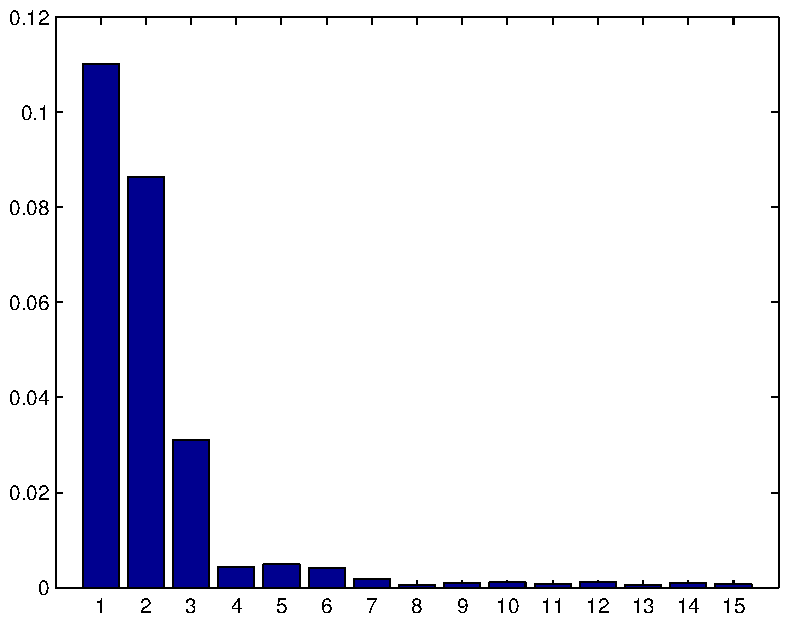
\includegraphics[width=0.145\textwidth]{../diagrams/Yale1Face/scales}
	\label{fig:yaleOneFaceScales}
}
\hspace{-5pt}
\subfigure[]{
	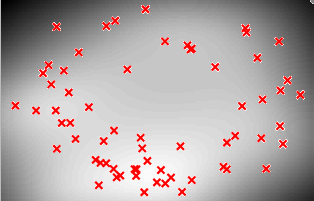
\includegraphics[width=0.145\textwidth]{../diagrams/Yale1Face/X21}
	\label{fig:yaleOneFaceX21}
}
\hspace{-5pt}
\subfigure[]{
	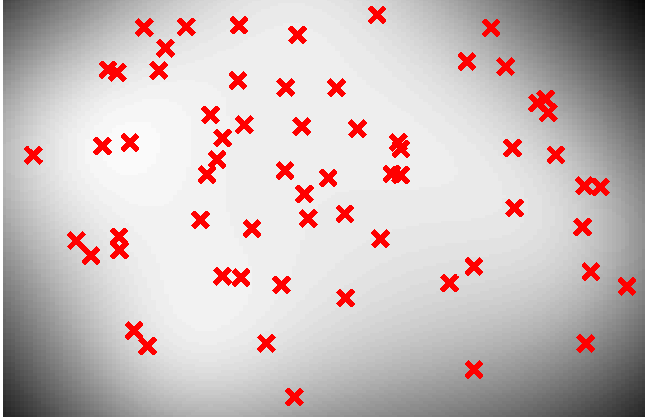
\includegraphics[width=0.145\textwidth]{../diagrams/Yale1Face/X23}
	\label{fig:yaleOneFaceX23}
}
\end{center}
\vspace{-7pt}
\caption{\small{ \it
The weight set $\bfw$ associated with the learned latent space is shown in \subref{fig:yaleOneFaceScales}.
In figures \subref{fig:yaleOneFaceX21} and \subref{fig:yaleOneFaceX23} we plotted pairs of the $3$ most dominant
latent dimensions against each other (dimension 1 against 2 and 1 against 3 respectively).
}
}
\label{fig:yaleOneFace1}
\vspace{-8pt}
\end{figure}
\hspace{-6pt}

This suggests that latent feature indices $1,2$ and $3$ encode the information about the illumination condition.
Figure \ref{fig:yaleOneFaceScales} also shows that the latent dimensions with indices $4,5$ and $6$ have a very small but not negligible weight.
%These are retained by the model because
%apart from the illumination condition, there exist other minor differences among pictures of a single face, as the depicted %persons
These represent other minor differences between an individual's face pictures, as the subjects
often blink, slightly move or smile etc. 



\subsubsection{Shared latent spaces for multiple faces}

In this section we use our model, from now on referred to as \emph{Manifold Relevance Determination model (MRD)} for latent subspace learning. 
We selected the pictures corresponding to all illumination conditions of $3$ subjects and created a dataset $Y$, and similarly
for $Z$ (for $3$ different subjects).
In this way, we formed two datasets, $Y$ and $Z$, each consisting of all $64 \times 3$ images corresponding to
a set of three different faces, therefore, $Y, Z \in \mathbb{R}^{N \times D}$, $N = 192$, $D = 32,256$.
 We then aligned the datasets, so that each image from the
first dataset was randomly set to correspond to one of the three faces of the second dataset which are depicted in the same illumination condition. In that way, the model is not
explicitly forced to learn the correspondence between face characteristics.

\par The MRD model was initialised by concatenating the two datasets and then performing PPCA in $Q=14$ dimensions. After training, 
the dimensions of the learned latent space are weighted by the parameters of the generative mappings $f_Y$ and $f_Z$ as shown in figure \ref{fig:yale6SetsScales}.

\begin{figure}[ht]
\begin{center}
\subfigure[]{
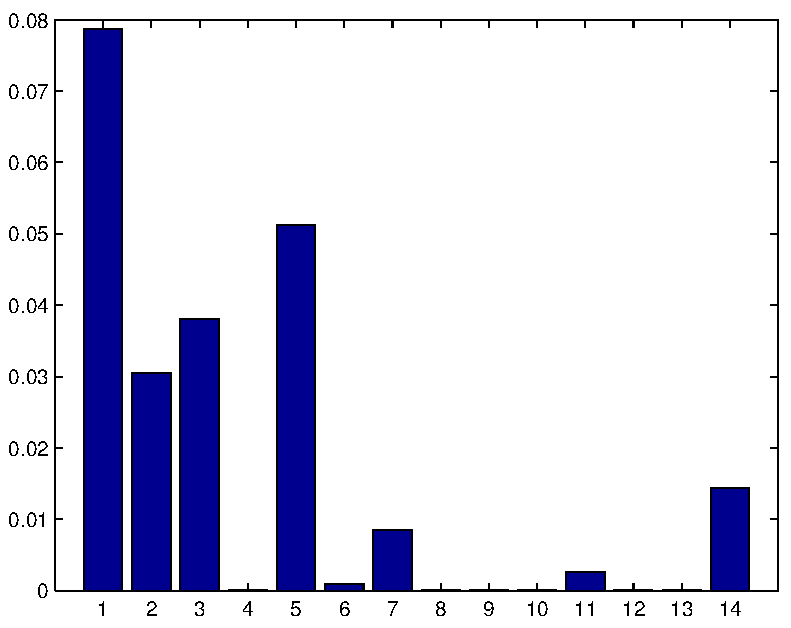
\includegraphics[width=0.18\textwidth]{../diagrams/Yale6Sets/scalesMod1}
	\label{fig:yale6SetsScales1}
}
\subfigure[]{
	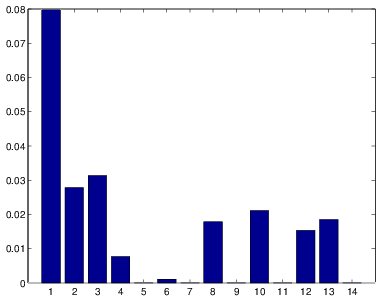
\includegraphics[width=0.18\textwidth]{../diagrams/Yale6Sets/scalesMod2}
	\label{fig:yale6SetsScales2}
}
\end{center}
\vspace{-9pt}
\caption{\small{ \it
The dimensions' weights, assigned for the first and second dataset 
in \subref{fig:yale6SetsScales1} and \subref{fig:yale6SetsScales2},
define a partitioning and ``soft'' sharing of the latent space. 
}}
\label{fig:yale6SetsScales}
\vspace{-8pt}
\end{figure}

The latent space is clearly segmented into a shared part, consisting of dimensions indexed as $1$,$2$ and $3$ 
\footnote{dimension 6 is also in the shared set but both models assigned a very small weight for that, as it encodes an almost negligible amount of information.}
and two private parts, consisting of dimensions indexed as $\{5,7,11,14 \}$ and $\{4,8,10,12,13 \}$ respectively. 
The $9$th feature of every latent point was found to be unnecessary for the generation of both output spaces.
What is more, 
the two models assigned almost (relatively) equal weights to the shared feature indices, and 
the shape of the shared latent space is similar to
the one found by the Bayesian GP-LVM (figure \ref{fig:yaleOneFace1}), as can be seen in figures \ref{fig:yale6SetsLatentSpace}\subref{fig:yale6SetsX12} and
\ref{fig:yale6SetsLatentSpace}\subref{fig:yale6SetsX13}.

This indicates that the shared space successfully encodes the information about
the position of the light source and not the face characteristics.
%as the random alignment that we performed forbade the algorithm from modelling commonalities between faces of the
%two different datasets.
 As for the private parts, these mainly correspond to disambiguating between faces of the same dataset. Indeed, plotting the largest two dimensions of
the first latent private subspace against each other reveals three clusters, corresponding to the three different faces within the dataset. 
Similarly to the standard Bayesian GP-LVM applied to a single face, here the private dimensions with the smaller weight
are the ones that model the minor differences introduced by the fact that the subject characteristics are slightly changed in several photos (due to blinking etc).

\hspace{-6pt}
\begin{figure}[ht]
\begin{center}
\subfigure[]{
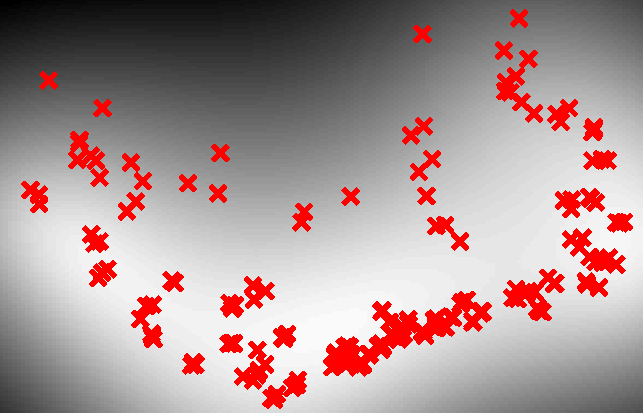
\includegraphics[width=0.145\textwidth]{../diagrams/Yale6Sets/mod1X_1_2}
	\label{fig:yale6SetsX12}
}
\hspace{-5pt}
\subfigure[]{
	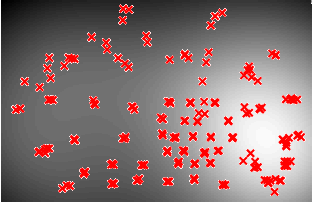
\includegraphics[width=0.145\textwidth]{../diagrams/Yale6Sets/mod1X_1_3}
	\label{fig:yale6SetsX13}
}
\hspace{-5pt}
\subfigure[]{
	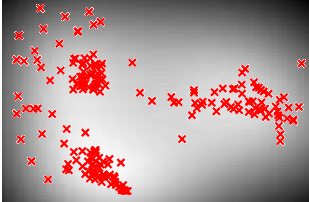
\includegraphics[width=0.145\textwidth]{../diagrams/Yale6Sets/mod1_X5_14}
	\label{fig:yale6SetsX5_14}
}
\end{center}
\vspace{-9pt}
\caption{\small{ \it
Projection of the shared latent space into dimensions $\{1,2\}$ and $\{1,3\}$ (figures
\subref{fig:yale6SetsX12} and \subref{fig:yale6SetsX13}) and projection of the $Y-$private dimensions $\{5,14\}$
(figure \subref{fig:yale6SetsX5_14}).
%which disambiguate between different faces in the first dataset.
 It is clear how the latent points in figure
\subref{fig:yale6SetsX5_14} form three clusters, each responsible for modelling one of the three faces in $Y$.
}}
\label{fig:yale6SetsLatentSpace}
\vspace{-8pt}
\end{figure}
\hspace{-6pt}


\par Given the above, it is obvious that the Manifold Relevance Determination model not only finds a very efficient and intuitive segmentation of the latent space, but it also
finds an effective dimensionality for each latent subspace. The Bayesian training allows for these procedures to be automated.

We can now confirm visually all of the subspaces' properties mentioned above and interpret their structure.
This is done by sampling a set of novel inputs $X_{samp}$ from each subspace and then mapping back to the observed data space using the
likelihood $p(Y|X_{samp})$, thus obtaining novel outputs (images).
%Being able to do so is an important advantage of our method (which is generative), because it also means that we can generate novel datapoints from the trained model.
%The intuitive segmentation of the latent space also helps towards this direction. 
To better understand what kind of information is encoded in each of the dimensions
of the shared or private spaces, we sampled new latent points by varying only one dimension at a time, while keeping the rest fixed. 

The first two rows of figure \ref{fig:yale6SetsInterpolation} show some of the outputs obtained after sampling across each of the shared dimensions $1$ and $3$ respectively, which clearly encode the coordinates of the light source,
whereas dimension $2$ was found to model the overall brightness. The sampling procedure can intuitively be thought as a walk in the space shown in figure \ref{fig:yale6SetsLatentSpace}\subref{fig:yale6SetsX13} from left to right and from the bottom to the top. Although the set of learned latent inputs is discrete, the corresponding latent subspace is continuous,
and we can interpolate images in new illumination conditions by sampling from areas where there are no training inputs (\ie in between the red crosses shown in figure \ref{fig:yale6SetsLatentSpace}).

% Using a generative model also allows us to sample new datapoints from the trained model. This is done by selecting a training input $\bfx_n$ (\ie one of
% the latent points corresponding to an existing, observed $\bfy_n$), and sampling one or more of its dimensions from the whole of the corresponding feature space,
% obtaining, thus, a novel input $\bfx_*$. We can then obtain novel outputs by using the likelihood $p(\bfy_n | \bfx_n)$. Figures \ref{}, \ref{} and \ref{} show some of the outputs obtained after
% sampling across each of the principle dimensions by hand. When the sampled $\bfx_*$ were close or exactly similar to training inputs, the corresponding output
% looks like one of the training datapoints, otherwise the output is novel. From the aforementioned figures, one can see that the two of the principal dimensions
% represent the change of the light source location along the $X$ and $Y$ axis respectively, whereas the third one is responsible for modelling the brightness.

Similarly, we can sample from the private subspaces and obtain novel outputs which interpolate the non-shared characteristics of the involved data. 
This results in a morphing effect across different faces, which is shown in the last row of figure \ref{fig:yale6SetsInterpolation}.
More examples and videos can be found in the supplementary material.


\begin{figure*}[ht]
\begin{center}
\subfigure{ 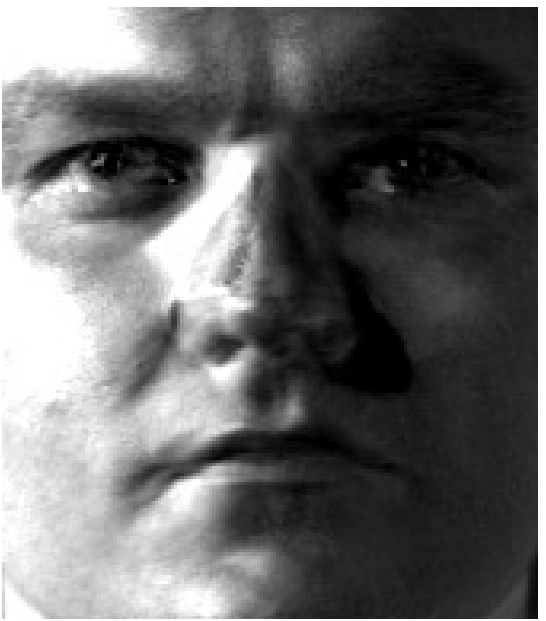
\includegraphics[width=0.09\textwidth]{../diagrams/Yale6Sets/lightInterpolation/X13_1000} }
\subfigure{ 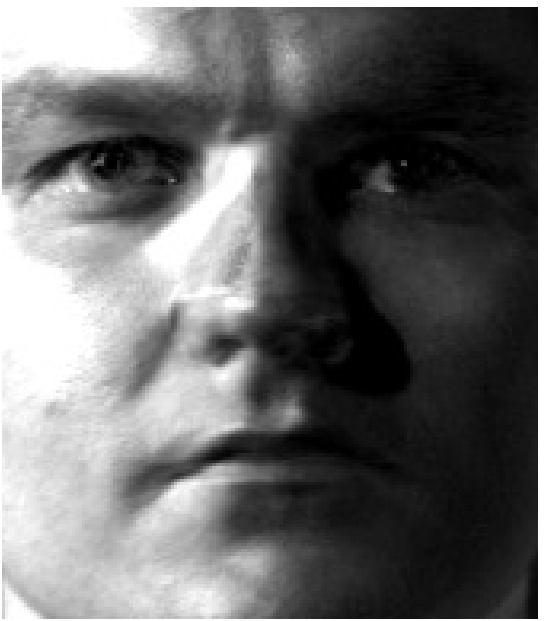
\includegraphics[width=0.09\textwidth]{../diagrams/Yale6Sets/lightInterpolation/X13_1009} }
\subfigure{ 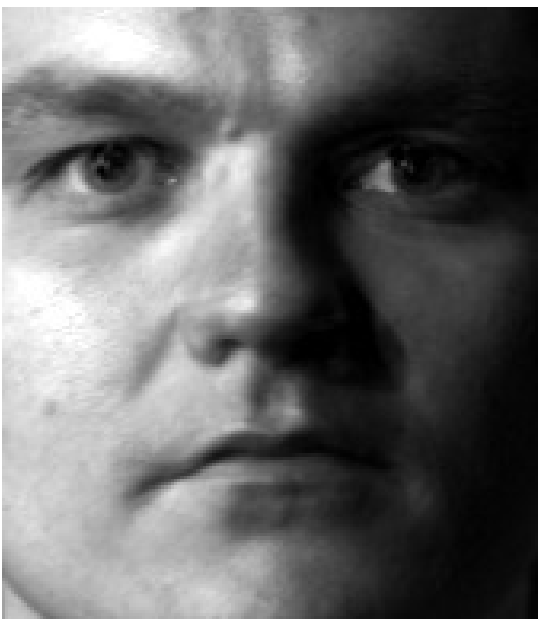
\includegraphics[width=0.09\textwidth]{../diagrams/Yale6Sets/lightInterpolation/X13_1021} }
\subfigure{ 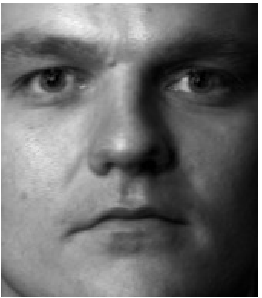
\includegraphics[width=0.09\textwidth]{../diagrams/Yale6Sets/lightInterpolation/X13_1022} }
\subfigure{ 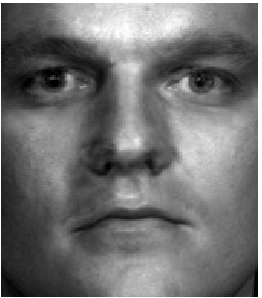
\includegraphics[width=0.09\textwidth]{../diagrams/Yale6Sets/lightInterpolation/X13_1036} }
\subfigure{ 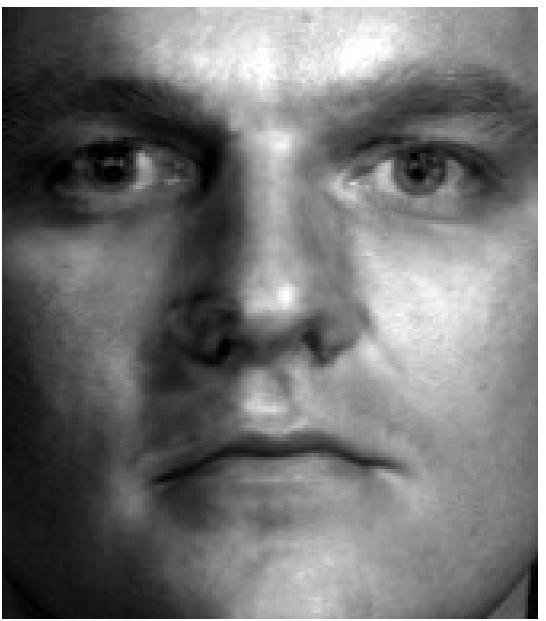
\includegraphics[width=0.09\textwidth]{../diagrams/Yale6Sets/lightInterpolation/X13_1040} }
\subfigure{ 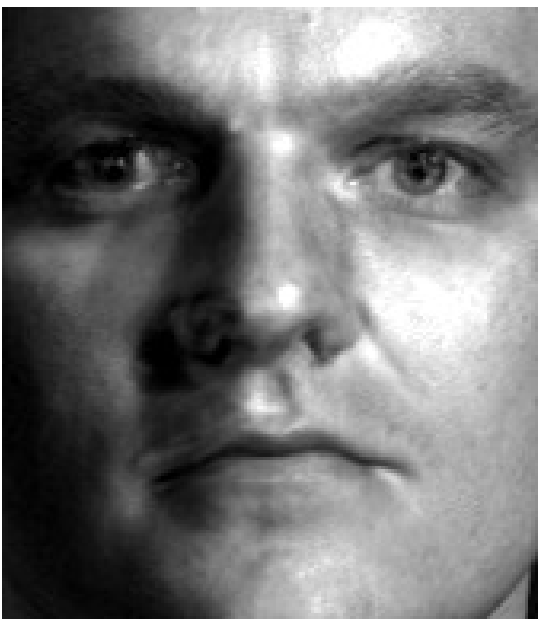
\includegraphics[width=0.09\textwidth]{../diagrams/Yale6Sets/lightInterpolation/X13_1046} }
\subfigure{ 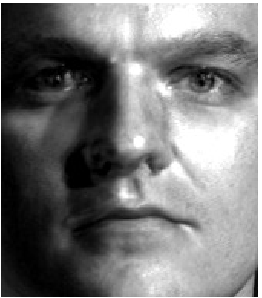
\includegraphics[width=0.09\textwidth]{../diagrams/Yale6Sets/lightInterpolation/X13_1055} }
\subfigure{ 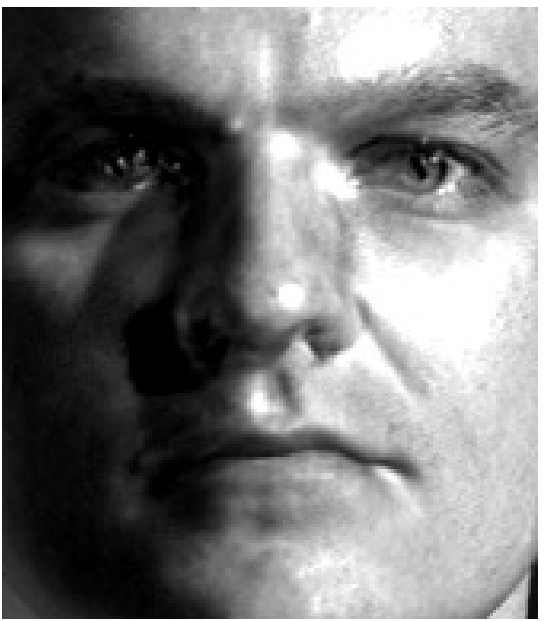
\includegraphics[width=0.09\textwidth]{../diagrams/Yale6Sets/lightInterpolation/X13_1063} }
\vspace{-8pt}
\newline
\subfigure{ 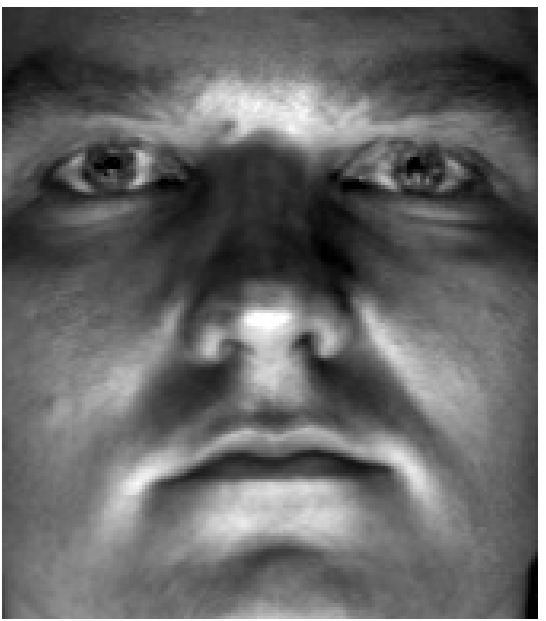
\includegraphics[width=0.09\textwidth]{../diagrams/Yale6Sets/lightInterpolation/X13_1064} }
\subfigure{ 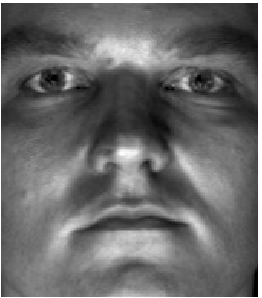
\includegraphics[width=0.09\textwidth]{../diagrams/Yale6Sets/lightInterpolation/X13_1072} }
\subfigure{ 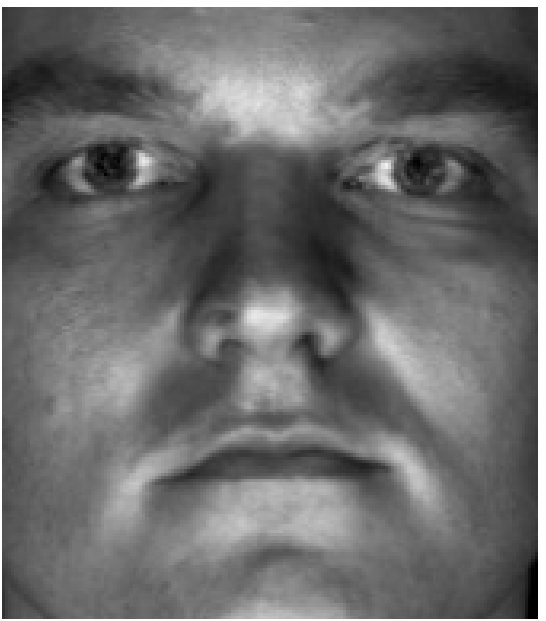
\includegraphics[width=0.09\textwidth]{../diagrams/Yale6Sets/lightInterpolation/X13_1079} }
\subfigure{ 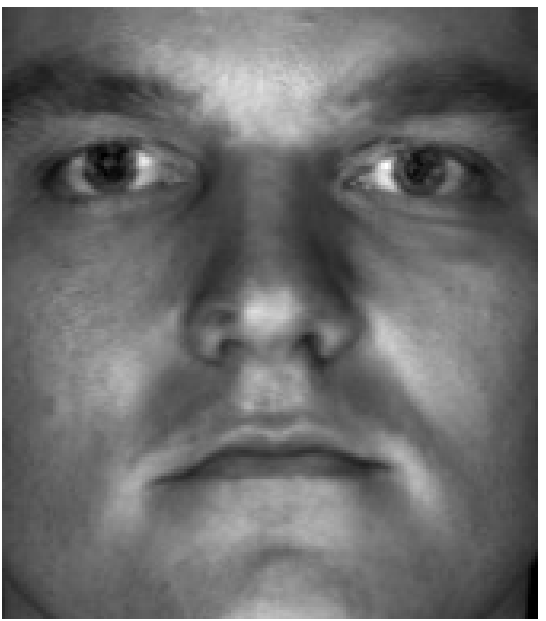
\includegraphics[width=0.09\textwidth]{../diagrams/Yale6Sets/lightInterpolation/X13_1085} }
\subfigure{ 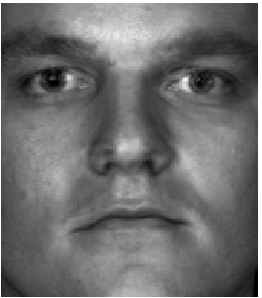
\includegraphics[width=0.09\textwidth]{../diagrams/Yale6Sets/lightInterpolation/X13_1095} }
\subfigure{ \includegraphics[width=0.09\textwidth]{../diagrams/Yale6Sets/lightInterpolation/X13_1110} }
\subfigure{ \includegraphics[width=0.09\textwidth]{../diagrams/Yale6Sets/lightInterpolation/X13_1125} }
\subfigure{ \includegraphics[width=0.09\textwidth]{../diagrams/Yale6Sets/lightInterpolation/X13_1137} }
\subfigure{ \includegraphics[width=0.09\textwidth]{../diagrams/Yale6Sets/lightInterpolation/X13_1149} }
\vspace{-8pt}
\newline
\subfigure{ \includegraphics[width=0.11\textwidth]{../diagrams/Yale6Sets/morphing/1054} }
\subfigure{ \includegraphics[width=0.11\textwidth]{../diagrams/Yale6Sets/morphing/1079} }
\subfigure{ \includegraphics[width=0.11\textwidth]{../diagrams/Yale6Sets/morphing/1089} }
\subfigure{ \includegraphics[width=0.11\textwidth]{../diagrams/Yale6Sets/morphing/1094} }
\subfigure{ \includegraphics[width=0.11\textwidth]{../diagrams/Yale6Sets/morphing/1102} }
\subfigure{ \includegraphics[width=0.11\textwidth]{../diagrams/Yale6Sets/morphing/1106} }
\subfigure{ \includegraphics[width=0.11\textwidth]{../diagrams/Yale6Sets/morphing/1123} }
\end{center}
\vspace{-4pt}
\caption{\small{ \it
Sampling inputs to produce novel outputs.
First row shows interpolation between positions of the light source in the $x$ coordinate
and second row in the $y$ coordinate (elevation). Last row shows interpolation between
face characteristics to produce a morphing effect.
}}
\label{fig:yale6SetsInterpolation}
\vspace{-8pt}
\end{figure*}




\par As a final test, we confirm the efficient segmentation of the latent space into private and shared parts by automatically recovering all the illumination similarities found in
the training set.
 More specifically, given a datapoint $\bfy_n$ from the first dataset, we search the whole space of training inputs $X$ to find the $6$ Nearest Neigbours to the latent representation 
$\bfx_n$ of $\bfy_n$, based only on the shared dimensions. 
%In other words, we compare $x_{n,i}$ to all the rest $\{x_{n,j}\}_{n=1}^N$, where $i \neq j$ and $i,j$ belong to the set
% of the shared dimensions. 
 From these latent points, we can then obtain points in the output space of the second dataset, by using the likelihood $p(Z | X)$.
 As can be seen in figure \ref{fig:yale6SetsGrouping}, the model returns images which match
the illumination condition of the given image. Moreover, the fact that, typically, the first
neighbours of each given point correspond to outputs belonging to different faces, also indicates that
the shared latent space is ``pure'', and it does not encode similarities of face characteristics.
%\hspace{-6pt}
\begin{figure}[ht]
\begin{center}
\subfigure{ \includegraphics[width=0.47\textwidth]{../diagrams/Yale6Sets/grouping/givenMod2/122} }
 \vspace{-16pt}
 \newline
\subfigure{ \includegraphics[width=0.47\textwidth]{../diagrams/Yale6Sets/grouping/givenMod2/107} }
 \vspace{-16pt}
 \newline
\subfigure{ \includegraphics[width=0.47\textwidth]{../diagrams/Yale6Sets/grouping/givenMod1/24} }
 \vspace{-16pt}
 \newline
\subfigure{ \includegraphics[width=0.47\textwidth]{../diagrams/Yale6Sets/grouping/givenMod1/70} }
 \vspace{-16pt}
 \newline
\end{center}
\vspace{-9pt}
\caption{\small{ \it
Given the images of the first column, the model searches only in the shared latent space to find the pictures of the opposite dataset
which have the same illumination condition. The images found, are sorted in columns
$2$ - $7$ by relevance.
}}
\label{fig:yale6SetsGrouping}
\vspace{-8pt}
\end{figure}

%\hspace{-6pt}

%%%% THE FIRST NN is the same latentn point, we should look from NN2 and so on.


\subsection{Human motion data}

For our second experiment, we consider 
a set of $3$D human poses and associated silhouettes,
coming from the dataset of Agarwal and Triggs \cite{Agarwal:pose06}. We used a subset of
$5$ sequences, totalling $649$ frames, corresponding to walking motions in various directions and patterns.
A separate walking sequence of $158$ frames was used as a test set.
Each pose is represented by a $63-$dimensional vector
of joint locations and each
silhouette is represented by a $100-$dimensional vector of HoG features.

\par Given the test silhouette features, we used our model to generate the corresponding
poses. This is a challenging task, since the data are multi-modal, \ie a silhouette representation
may be generated from more than one poses (\eg figure \ref{fig:humanPoseAmbiguity}). 

\begin{figure}[ht]
\begin{center}
%  \includegraphics[width=0.43\textwidth]{../diagrams/humanPose/ambiguity2FinalCombined3}
  \includegraphics[width=0.35\textwidth]{../diagrams/humanPose/newAmbiguity}
\end{center}
\vspace{-9pt}
\caption{\small{ \it
Although the two poses in the second column are very dissimilar, they correspond to resembling silhouettes
that have similar feature vectors. This happens because the $3$D information is lost in the silhouette space,
as can also be seen in the third column, depicting the same poses from the silhouettes' viewpoint.}}
\label{fig:humanPoseAmbiguity}
\vspace{-4pt}
\end{figure}

As described in section \ref{inference}, given $\bfy^*$, one of the $N_*$ test silhouettes, our model optimises a test latent point $\bfx^*$ and finds
 a series of $K$ candidate initial training inputs $ \{ \bfx_{NN}^{(k)} \}_{k=1}^K$, sorted according to their similarity to $\bfx^*$, taking into account only the shared dimensions. 
 Based on these initial latent points, it then generates a sorted series of $K$ poses $\{ \bfzi^{(k)} \}_{k=1}^K$. For the dynamical version of our model,
all the test points are considered together and the predicted $N_*$ outputs are forced to form a smooth sequence.
 Our experiments showed that the initial training inputs $\bfx_{NN}$ typically correspond to silhouettes similar to the given one, something which
 confirms that the segmentation of the latent space is efficient. However, when ambiguities arise, as the example
 shown in figure \ref{fig:humanPoseAmbiguity}, the non-dynamical version of our model has no way of selecting the right one, since all points
 of the test sequence are treated independently. But when the dynamical version is employed, the model forces the whole set of training and test inputs to create smooth paths in the latent space, as can be seen in figure \ref{fig:humanPoseLatentSpaces}. In other words,
 the dynamics disambiguate the model.  

\begin{figure}[ht]
\begin{center}
\subfigure[]{ \includegraphics[width=0.18\textwidth]{../diagrams/humanPose/latentSpaceStatic} 
\label{fig:latentSpaceStatic}
} \hspace{-3pt}
\subfigure[]{ \includegraphics[width=0.18\textwidth]{../diagrams/humanPose/latentSpaceDynCropped} 
\label{fig:latentSpaceDyn}
}
\end{center}
\vspace{-9pt}
\caption{\small{ \it Projection of the latent space discovered for the non-dynamical model \subref{fig:latentSpaceStatic}
and for the dynamical model \subref{fig:latentSpaceDyn} onto their two principal dimensions.
}
}
\label{fig:humanPoseLatentSpaces}
\vspace{-3pt}
\end{figure}


Indeed, as can be seen in figure \ref{fig:humanPoseAmbiguityTest}, our method is forced to select a candidate training input $\bfx_{NN}$ for initialisation which does not necessarily
correspond to the training silhouette that is most similar to the test one. 
%
%In other words, the predicted pose is generated by a latent point which is not
%necessarily initialised in the latent point that is found by Nearest Neighbour in the silhouette space. 
%
What is more, if we assume that the test \emph{pose} $\bfzi^*$ is known and seek for its nearest training neighbour in the pose space, we find that the corresponding silhouette
is very similar to the one found by our model, which is only given information in the silhouette space.

\begin{figure}[ht]
\begin{center}
  \includegraphics[width=0.35\textwidth]{../diagrams/humanPose/ambiguityTest}
\end{center}
\caption{\small{\it Given the HoG features for the test silhouette in column one, we predict the corresponding pose using the dynamical version of MRD and Nearest Neighbour in the silhouette space
obtaining the results in the first row, columns 2 and 3 respectively. The last row is the same as the first one, but the poses are rotated
to highlight the ambiguities. Notice that the silhouette shown in the second row for MRD does not correspond exactly to the pose
of the first row, as the model generates only the pose given a test silhouette. Instead, it is the training silhouette which MRD chose to initialise with, by performing
Nearest Neighbour in the shared latent space. 
We also found the Nearest Neighbour of the training \emph{pose} (column 4) given the test pose, so as to show that the corresponding silhouette is very similar to the one
selected by MRD for initialisation.
}}
\label{fig:humanPoseAmbiguityTest}
\end{figure}

\par Given the above, we quantify the results and compare our method
with linear and Gaussian process regression and Nearest Neighbour in the silhouette space. We also compared against
the Shared GP-LVM \cite{Ek:2008up, Ek:2009vv} which optimises the latent points using MAP and, therefore, requires an initial factorisation
of the inputs to be given a priori. 
The errors shown in table \ref{humanMotionTable} as well as the video provided as supplementary  material show that MRD
performs better than the other methods in this task.



\begin{table}[h]
\label{humanMotionTable}
\begin{center}
\begin{tabular}{|l|l|}
\hline
						 	   & Error \\ \hline \hline
Mean Training Pose		       & 6.16   \\ \hline
Linear Regression		       & 5.86   \\ \hline
GP Regression 			       & 4.27   \\ \hline
Nearest Neighbour (sil. space) & 4.88  \\ \hline
\textcolor{Gray}{Nearest Neighbour (pose space)} & \textcolor{Gray}{2.08}   \\ \hline
Shared GP-LVM				       & 5.13    \\ \hline
MRD	without Dynamics       & 4.67   \\ \hline
MRD with Dynamics	       & \textbf{2.94}    \\ \hline
\end{tabular}
\end{center}
\caption{
\small{ \it
The mean of the Euclidean distances of the joint locations between the predicted and the true poses.
The Nearest Neighbour in the pose space
is not a fair comparison, but is reported here as it provides some insight about the
lower bound on the error that can be achieved for this task.
}}
\end{table}









\section{Conclusions \label{conclusions}}
%% Many applications in computer vision and related fields are concerned
%% with modelling in scenarios where multiple streams of information of
%% the same underlying phenomenon are available. Further, the data is
%% often very high dimensional with enormous redundancies.
%Such a representation often means that the data
%is distributed on or close to a manifold through the observed
%parametrization.  
We have presented a new factorized latent variable model for multi
view data.  The model automatically factorizes the data using
variables representing variance that exists in each view separately
from variance being specific to a particular view. 
%% that automatically factorizes the latent space into variables that
%% are either shared or specific to one of the views of the
%% data.
% We introduced a relaxation to the discrete segmentation
%% of the latent representation 
% and allow for a ``softly'' shared latent space.
%The model learns the structure of the latent space variationally,
% allowing it to incorporate prior distributions for the latent space. 
The model learns a distribution over the latent points
variationally. This allows us to to automatically find the
dimensionality of the latent space as well as to incorporate prior
knowledge about its structure.
%
As an example, we showed how dynamical priors can be included on the latent
space. This allowed us to use temporal continuity to disambiguate the
model's predictions in an ambiguous human pose estimation problem.
%
%We exploited the factorization to perform human
%pose estimation in an ambiguous setting.
% where the model separates the variance in the pose
%space that can be determined from the image observations from the one
%that is ambiguous. 
% Our model allows for dynamical priors to be
% incorporated when learning it. This allowed us to disambiguate
% in the pose estimation example. 
%
The model is capable of learning from extremely high-dimensional
data. We illustrated this by learning a model directly on the pixel
representation of an image. Our model is capable of learning a compact
an intuitive representation of such data which we exemplified by
generating novel images by sampling from the latent representation in a
structured manner.
%% applying it to images of several different
%% faces under the same set of lighting conditions. Images of faces from
%% novel lighting directions or with novel appearance could be
%% synthesized by sampling from the corresponding latent space.
%
%The model is capable of learning from
%extremely high-dimensional data. By applying it to images of
%several different faces under the same set of lighting conditions the model
%correctly finds the generating low-dimensional parameters of the data
%separated into facial appearance and illumination direction. From the
%resulting model we showed how images of faces from novel lighting
%directions or with novel facial characteristics could be synthesized.
%
%
Finally, we showed how a generative model with discriminative
capabilities can be obtained by treating the observations and class labels
of a dataset as separate modalities.  

% As future work, we envisage
% approaches with more sophisticated ways of directly constraining the
% latent space through priors. 
% %In classification scenarios, for
% %example, we could consider a latent space prior evaluated at the class
% %labels.
%  Further, it would be interesting to explore the possibility of
% incorporating different latent space constraints for each different
% observed modality.


%%% Local Variables: 
%%% mode: latex
%%% TeX-master: "../svargplvmICML2012"
%%% End: 










%----------------------------------------------- ACKNOWLEDMENTS -----------------------------------------
\subsubsection*{Acknowledgments}
Research was partially supported by the University of Sheffield Moody endowment fund and the Greek State
 Scholarships Foundation (IKY).
We also thank Colin Litster and ``Fit Fur Life'' for allowing us to use their video files as datasets.

%\bibliographystyle{apalike}
%\bibliographystyle{ieeetr}
\bibliographystyle{abbrvnat}
\renewcommand*{\refname}{\begin{normalsize}References\end{normalsize}}
\bibliography{vargplvm,lawrence,other,zbooks}
%\singlespace
%\bibliography{paper}





\newpage
 \begin{center}
 \begin{Large}
 \textbf{
% Gaussian Process Dynamical Systems\\
 Appendix
 } \\
 \end{Large}
% \noindent \newline
% \textbf{Andreas Damianou, Michalis Titsias, Neil Lawrence}
 \end{center}
\appendix
\section{Derivation of the variational bound}

We wish to approximate the marginal likelihood:
\begin{equation}
\label{marginalLikelihoodSuppl}
p(Y | \bft) =  \int p( Y , F, X| \bft) \intd  X \intd F,
\end{equation}
by computing a lower bound:
\begin{align}
\mathcal{F}_v(q, \boldsymbol \theta) = {}& \int q(\mathit{\Theta}) \log 
		\frac{ p(Y , F , \mathit{X} | \mathbf{t})}
			 {q(\mathit{\Theta})}  \intd  X \intd F.
% 	    \nonumber \\
% 	      = {}& \sum_{d=1}^D \int q(\Theta) \log \left( p(\bfy_d | \bff_d) p(\bff_d | X) \right) dX d \bff_d -
% 		    \int q(\Theta) \frac{p(X|\bft)}{q(\Theta)} dX
		 \label{jensens1Suppl}
\end{align}
%
This can be achieved by first augmenting the joint probability density of our model with inducing inputs $\tilde{X}$ along with their corresponding function values $U$:
\begin{equation}
 \label{augmentedJointSuppl}
p(Y,F, U,X,\tilde{X} | \bft) = \prod_{d=1}^D p(\mathbf{y}_d | \mathbf{f}_d) p(\mathbf{f}_d | \mathbf{u}_d, \mathit{X})
p(\bfu_d | \tilde{X})  p(X | \mathbf{t})
\end{equation}
where $p(\bfu_d | \tilde{X}) = \prod_{d=1}^D \mathcal{N} \left( \bfu_d | \mathbf{0}, K_{MM} \right)$ . For simplicity, $\tilde{X}$ is dropped from our
expressions for the rest of this supplementary material. Note that after including the inducing points, $p(\bff_d | \bfu_d, X)$
remains analytically tractable and it turns out to be \cite{rasmussen-williams}):
\begin{equation}
 \label{priorF2Suppl}
p(\bff_d | \bfu_d, X) =  \mathcal{N}  \left( \bff_d | K_{NM} K_{MM}^{-1} \bfu_d , K_{NN} - K_{NM} K_{MM}^{-1} K_{MN} \right).
\end{equation}
For tractability, we now define a variational density $q(\Theta)$:
\begin{equation}
\label{varDistrSuppl}
q(\mathit{\Theta}) = q(F, U,X) = q(F | U, X) q(U) q(X) = \prod_{d=1}^D p(\bff_d | \bfu_d, X )q(\bfu_d) q(X),
\end{equation}
%
%
where $q(X) = \prod_{q=1}^Q \mathcal{N} \left( \bfx_q | \bfmu_q, S_q \right)$. 
%
Now, we return to \eqref{jensens1Suppl} and replace the joint distribution with its augmented version \eqref{augmentedJointSuppl} and the variational distribution with its factorised version \eqref{varDistrSuppl}:
\begin{align}
\mathcal{F}_v(q, \boldsymbol \theta) = {}& \int q(\mathit{\Theta}) \log 
		\frac{ p(Y,F, U,X | \bft)}
			 {q(F, U,X)}  \intd  X \intd F,
 	    \nonumber \\
= {}& \int \prod_{d=1}^D p(\bff_d | \bfu_d, X )q(\bfu_d) q(X) 
	    \log  \frac{\prod_{d=1}^D p(\mathbf{y}_d | \mathbf{f}_d) \cancel{p(\mathbf{f}_d | \mathbf{u}_d, \mathit{X})}
						p(\bfu_d | \tilde{X})  p(X | \mathbf{t})}
 	      		   {\prod_{d=1}^D \cancel{p(\bff_d | \bfu_d, X )}q(\bfu_d) q(X)}   \intd  X \intd F \nonumber \\
= {}& \int \prod_{d=1}^D p(\bff_d | \bfu_d, X )q(\bfu_d) q(X) 
		\log  \frac{\prod_{d=1}^D p(\mathbf{y}_d | \mathbf{f}_d) p(\bfu_d | \tilde{X})}
				   {\prod_{d=1}^D q(\bfu_d) q(X)}   \intd  X \intd F \nonumber \\
- {}& \int \prod_{d=1}^D  q(X)   \log \frac{q(X)}{p(X | \mathbf{t})}   \intd  X \nonumber \\
= {}& \hat{\mathcal{F}}_v - \text{KL}(q \parallel p), \label{jensensSuppl}
\end{align}
%
with:
 \begin{equation}
\hat{\mathcal{F}}_v = 
\sum_{d=1}^D \left( 
    \int q(\bfu_d) q(X) \left\langle \log p(\bfy_d | \bff_d) \right\rangle_{p(\bff_d | \bfu_d, X)} d\bfu_d \; dX +
					   \log \left\langle \frac{p(\bfu_d)}{q(\bfu_d)} \right\rangle_{q(\bfu_d)} 
  \right) = \sum_{d=1}^D \hat{\mathcal{F}}_d
\end{equation} 

Both terms in \eqref{jensensSuppl} are analytically tractable, with the first having the same analytical solution as the one derived in \cite{BayesianGPLVM}. Further calculations in the the $\hat{\mathcal{F}}_v$ term reveal that the optimal setting for $q(\bfu_d)$ is also a Gaussian. More specifically, 
we have:
\begin{align}
\hat{\mathcal{F}}_v={}& \int q(\bfu_d) \log \frac{e^{\la \log N \left( \bfy_d | \bfa_d, \beta^{-1} I_d \right) \ra_{q(X)}}
		p(\bfu_d)}{q(\bfu_d)} d\bfu_d - A \label{boundFAnalytically5}
\end{align}
where $A$ is a collection of remaining terms and $\bfa_d$ is the mean of \eqref{priorF2Suppl}.
\eqref{boundFAnalytically5} is a KL-like quantity and, therefore, $q(\bfu_d)$ is optimally set to be the quantity appearing in the numerator of the above equation. So:
%:
% \begin{equation}
% q(\bff_{*,d}^m | X_*) = \mathcal{N}(\bff_{*,d}^m| \beta K_{N_* M} 
% (K_{MM} + \beta \Psi_2)^{-1} \Psi_1^{T} \bfy_d, K_{N_* N_*} - 
%  K_{N_* M} \left[ K_{M M}^{-1}  - (K_{M M} + \beta \Psi_2)^{-1} \right] 
%  K_{N_* M}^{T}),
% \end{equation}
% exactly as in \cite{BayesianGPLVM}.
\begin{equation}
\label{qu}
q(\bfu_d) = e^{\la \log \mathcal{N} \left( \bfy_d | \bfa_d, \beta^{-1} I_d \right) \ra_{q(X)}}
		p(\bfu_d) ,
\end{equation}
exactly as in \cite{BayesianGPLVM}. This is a Gaussian distribution since $p(\bfu_d ) = \mathcal{N} (\bfu_d | \mathbf{0}, K_{MM} )$.

\par
The complete form of the Jensen's lower bound turns out to be:
\begin{align}
\mathcal{F}_v(q, \boldsymbol \theta) = {}& \sum_{d=1}^{D} 
	\hat{\mathcal{F}}_d(q, \boldsymbol \theta) -  \text{KL}(q \parallel p) \nonumber \\
	= {}& 
	\sum_{d=1}^{D} 
		\log \left( 
		\frac{(\beta)^{\frac{N}{2}} \vert \mathit{K_{MM}} \vert ^\frac{1}{2} }
			 {(2\pi)^{\frac{N}{2}} \vert \beta \Psi_2 + \mathit{K_{MM}}  \vert ^\frac{1}{2} } 	
		 e^{-\frac{1}{2} \mathbf{y}^{T}_{d} W \mathbf{y}_d} 
		 \right) -
		 \frac{\beta \psi_0}{2} + \frac{\beta}{2} 
		 \text{Tr} \left( \mathit{K_{MM}^{-1}} \Psi_2 \right)  \nonumber \\
{}&	- \frac{Q}{2} \log \vert \mathit{K_t} \vert - \frac{1}{2} \sum_{q=1}^{Q}
	  \left[ \text{Tr} \left( \mathit{K_t}^{-1} \mathit{S_q} \right)	  
	  	   + \text{Tr} \left( \mathit{K_t}^{-1} \boldsymbol \mu_q \boldsymbol \mu_q^T \right) \right] 
	 + \frac{1}{2} \sum_{q=1}^Q \log \vert \mathit{S_q} \vert + const  \label{boundFinal}
\end{align}
where the last line corresponds to the KL term. Also:
\begin{equation}
\label{psis}
\Psi_0 = \text{Tr}(\langle \mathit{K_{NN}} \rangle_{q(\mathit{X})}) \;, \;\;
\Psi_1 = \langle \mathit{K_{NM}} \rangle_{q(\mathit{X})} \;, \;\;
\Psi_2 = \langle \mathit{K_{MN}} \mathit{K_{NM}} \rangle_{q(\mathit{X})}
\end{equation}
The $\Psi$ quantities can be computed analytically as in \cite{BayesianGPLVM}.


%-------------------------

\section{Derivatives of the variational bound}
Before giving the expressions for the derivatives of the variational bound \eqref{jensensSuppl},
it should be reminded that the variational parameters $\mu_q$ and $S_q$ (for all $q$s) have been
reparametrized as $S_q = \left( \mathit{K}_t^{-1} + diag(\boldsymbol \lambda_q) \right)^{-1}  \text{ and }   \boldsymbol \mu_q = K_t \bar{\boldsymbol \mu}_q$, where the function $diag(\cdot)$ transforms a vector into a square diagonal matrix and vice versa. Given the above, the set of the parameters to be optimised is 
$( \boldsymbol \theta_f, \boldsymbol \theta_x, \{ \bar{\bfmu}_q, \boldsymbol \lambda_q \}_{q=1}^Q, \tilde{X})$. The gradient w.r.t the inducing points $\tilde{X}$, however, has exactly the same form as for $\boldsymbol \theta_f$ and, therefore, is not presented here. Also notice that from now on we will often use the term ``variational parameters'' to refer to the new quantities $\bar{\bfmu}_q$ and $\boldsymbol \lambda_q$. 

\textbf{Some more notation:} 
\begin{enumerate}
\item $\lambda_q$ is a scalar, an element of the vector $\boldsymbol \lambda_q$ which, in turn, is the main diagonal of the diagonal matrix $\Lambda_q$. 
%\item$\lambda_m \triangleq \boldsymbol \lambda_{q;m}$, i.e. the $m$-th element of the vector $\boldsymbol \lambda_q$ (thus, an instantiation of $\lambda_q$)
\item $S_{ij} \triangleq S_{q;ij}$ the element of $S_q$ found in the $i$-th row and $j$-th column.
\item $\mathbf{s}_q \triangleq \lbrace S_{q;ii} \rbrace_{i=1}^N$, i.e. it is a vector with the diagonal of $S_q$.
%\item $s_i$ is the $i$-th element of $\mathbf{s}_q$.
%\item $diag(\mathbf{s}_q)$ is a matrix full of zeros apart from the main diagonal which contains the vector $\mathbf{s}_q$.
\end{enumerate}

\subsection{Derivatives w.r.t the variational parameters}
\begin{equation}
    \label{derivVarParamSuppl}
\frac{\vartheta \mathcal{F}_v}{\vartheta \bar{\boldsymbol \mu}_q} 
=  K_t \left( \frac{\vartheta \hat{\mathcal{F}}_v}{\vartheta \boldsymbol \mu_q} - \bar{\boldsymbol \mu}_q \right)
\text{ and }
 \frac{\vartheta \mathcal{F}_v}{\vartheta \boldsymbol \lambda_q}
= - ( S_q \circ S_q) \left( \frac{\vv \hat{\mathcal{F}}_v}{\vv \mathbf{s}_q} + \frac{1}{2} \boldsymbol \lambda_q \right).
\end{equation}

where $\circ$ denotes the Hadamard product and:

\begin{align}
 \frac{\hat{\mathcal{F}_v}(q, \boldsymbol \theta)}{\vartheta \mu_q}
{}& = - \frac{\beta D}{2} \frac{\vartheta \Psi_0}{\vartheta \mu_q}
    + \beta \text{Tr} \left(\frac{\vartheta \Psi_1^T}{\vartheta \mu_q} Y Y^T \Psi_1 A^{-1} \right) \nonumber \\
{}& + \frac{\beta}{2} \text{Tr} \left[ \frac{\vartheta \Psi_2}{\vartheta \mu_q}
       \left(
	  D K_{MM}^{-1} - \beta^{-1} D A^{-1} - A^{-1} \Psi_1^T Y Y^T \Psi_1 A^{-1}
       \right) \right] \label{derivFTildeEfficientComputationMu}
\end{align}


\begin{align}
 \frac{\vv \hat{\mathcal{F}_v}(q, \boldsymbol \theta)}{\vartheta S_{q;i,j}}
{}& = - \frac{\beta D}{2} \frac{\vartheta \Psi_0}{\vartheta S_{q;i,j}}
    + \beta \text{Tr} \left(\frac{\vartheta \Psi_1^T}{\vartheta S_{q;i,j}} Y Y^T \Psi_1 A^{-1} \right) \nonumber \\
{}& + \frac{\beta}{2} \text{Tr} \left[ \frac{\vartheta \Psi_2}{\vartheta S_{q;i,j}}
       \left(
	  D K_{MM}^{-1} - \beta^{-1} D A^{-1} - A^{-1} \Psi_1^T Y Y^T \Psi_1 A^{-1}
       \right) \right] \label{derivFTildeEfficientComputationS}
\end{align}


with $A=\beta^{-1}K_{MM}+\Psi_2$.


%-------



\subsection{Derivatives w.r.t $\boldsymbol \theta = (\boldsymbol \theta_f, \boldsymbol \theta_x)$ and $\beta$}
Given that the KL term involves only the temporal prior, its gradient w.r.t the parameters $\boldsymbol \theta_f$ is zero. Therefore:
\begin{equation}
   \label{DerivativeOfFComplete}
      \frac{\vartheta \mathcal{F}_v}{\vartheta \theta_f} = \frac{\vartheta \hat{\mathcal{F}}_v}{\vartheta \theta_f}
\end{equation}

  with:

\begin{align}
\frac{\vartheta \hat{\mathcal{F}}_v}{\vartheta \theta_f} {}& = \text{const} - 
\frac{\beta D}{2} \frac{\vartheta \Psi_0}{\vartheta \theta_f}
 + \beta \text{Tr} \left(\frac{\vartheta \Psi_1^T}{\vartheta \theta_f} Y Y^T \Psi_1 A^{-1} \right) \nonumber \\
{}& + \frac{1}{2} \text{Tr} \left[ \frac{\vartheta K_{MM}}{\vartheta \theta_f}
        \left(
	   D K_{MM}^{-1} - \beta^{-1} D A^{-1} - A^{-1} \Psi_1^T Y Y^T \Psi_1 A^{-1} - \beta D K_{MM}^{-1} \Psi_2 K_{MM}^{-1} 
         \right) \right] \nonumber \\
{}& + \frac{\beta}{2} \text{Tr} \left[ \frac{\vartheta \Psi_2}{\vartheta \theta_f} \;\;\;\;
       \left(
	  D K_{MM}^{-1} - \beta^{-1} D A^{-1} - A^{-1} \Psi_1^T Y Y^T \Psi_1 A^{-1}
       \right) \right] \label{DerivativeOfFtildeComplete}
\end{align}

The expression above is identical for the derivatives w.r.t the inducing points.
For the gradients w.r.t the $\beta$ term, we have a similar expression:



\begin{align}
\frac{\vartheta \hat{\mathcal{F}}_v}{\vartheta \beta} ={}&
  \frac{1}{2} \Big[ 
      D \left( \text{Tr}(K_{MM}^{-1} \Psi_2) + (N-M)\beta^{-1} - \Psi_0 \right) - \text{Tr}(Y Y^\T)
	  + \text{Tr}(A^{-1}\Psi_1^\T Y Y^\T \Psi_1) \nonumber \\
   +{}& \beta^{-2} D \text{Tr} ( K_{MM} A^{-1} ) + \beta^{-1} \text{Tr} \left( K_{MM}^{-1} A^{-1} \Psi_1^\T Y Y^\T \Psi_1 A^{-1} \right) \Big]
\label{derivb2}
\end{align}


In contrast to the above, the term $\hat{\mathcal{F}}_v$ does involve parameters $\boldsymbol \theta_x$, because it involves the variational parameters that are now reparametrized with $K_t$, which in turn depends on $\boldsymbol \theta_x$. 
To demonstrate that, we will forget for a moment the reparametrization of $S_q$ and we will express the bound as $F(\boldsymbol \theta_x, \mu_q (\boldsymbol \theta_x))$ (where $\mu_q (\boldsymbol \theta_x) = K_t \bar{\boldsymbol \mu_q}$) so as to show explicitly the dependency on the variational mean which is now a function of $\boldsymbol \theta_x$. Our calculations must now take into account the term
$
\left( \frac{\vartheta \hat{\mathcal{F}}_v(\boldsymbol \mu_q)}{\vartheta \boldsymbol \mu_q} \right)^\T
       \frac{\vartheta \mu_q (\boldsymbol \theta_x)}{\vartheta \boldsymbol \theta_x}
$
that is what we ``miss'' when we consider $\mu_q(\boldsymbol \theta_x) = \boldsymbol \mu_q$:
\begin{align}
\frac{\vartheta \mathcal{F}_v(\boldsymbol \theta_x, \mu_q(\boldsymbol \theta_x))}{\vartheta \theta_x} = {}&
	\frac{\vartheta \mathcal{F}_v(\boldsymbol \theta_x, \boldsymbol \mu_q)}{\vartheta \theta_x} 
  +  \left( \frac{\vartheta \hat{\mathcal{F}}_v(\boldsymbol \mu_q)}{\vartheta \boldsymbol \mu_q} \right)^\T
            \frac{\vartheta \mu_q(\boldsymbol \theta_x)}{\vartheta \theta_x} \nonumber \\
= {}&
 \cancel{
    \frac{\vartheta \hat{\mathcal{F}}_v(\boldsymbol \mu_q)}{\vartheta \theta_x}
  } +
  \frac{\vv (-\text{KL})(\boldsymbol \theta_x, \boldsymbol \mu_q(\boldsymbol \theta_x))}{\vartheta \theta_x}
+  \left( \frac{\vartheta \hat{\mathcal{F}}_v(\boldsymbol \mu_q)}{\vartheta \boldsymbol \mu_q} \right)^\T
            \frac{\vartheta \mu_q(\boldsymbol \theta_x)}{\vartheta \theta_x}
\label{meanReparamDerivFTheta}
\end{align}

We do the same for $S_q$ and then we can take the resulting equations and replace $\bfmu_q$ and $S_q$ with their equals so as to obtain the final expression which only contains $\bar{\bfmu}_q$ and $\boldsymbol \lambda_q$:

\begin{align}
\frac{\vartheta \mathcal{F}_v(\boldsymbol \theta_x, \mu_q(\boldsymbol \theta_x), S_q(\boldsymbol \theta_x))}{\vartheta \theta_x}
={}& \text{Tr} \bigg[
\Big[ - \frac{1}{2} \left( \hat{B}_q K_t \hat{B}_q + \bar{\bfmu}_q \bar{\bfmu}_q^\T \right) \nonumber \\
+{}& \left( I - \hat{B}_q K_t \right)
 diag \left(  \frac{\vv \hat{\mathcal{F}}_v}{\vv \mathbf{s}_q} \right)
			 \left( I - \hat{B}_q K_t \right)^\T \Big]
			  \frac{\vv K_t}{\vv \theta_x} \bigg] 	\nonumber \\	
+{}&  \left( \frac{\vartheta \hat{\mathcal{F}}_v( \boldsymbol \mu_q)}{\vartheta \boldsymbol \mu_q} \right)^\T
					\frac{\vv K_t}{\vv \theta_x} \bar{\boldsymbol \mu}_q 
\label{CompleteBoundDerivThetatB}
\end{align}
where $\hat{B}_q = \Lambda_q^{\frac{1}{2}} \widetilde{B}_q^{-1} \Lambda_q^{\frac{1}{2}}$.
and $\tilde{B}_q = I + \Lambda_q^{\frac{1}{2}} K_t \Lambda_q^{\frac{1}{2}}$. Note that by using this
$\tilde{B}_q$ matrix (which has eigenvalues bounded below by one) we have an expression which, when implemented, leads to more numerically stable computations, as explained in \cite{rasmussen-williams} page 45-46. 




\section{Predictions}


\subsection{Predictions given only the test time points \label{supplUnobservedData}}
%Firstly, we discuss how the model can predict or generate a set of outputs $Y_*$ given only an input time-vector $\bft_*$. 
To approximate the predictive density, we will need to introduce the underlying latent function values $F_* \in \mathbb{R}^{N_* \times D}$ (the noisy-free version of $Y_*$) and the latent variables $X_* \in \mathbb{R}^{N_* \times Q}$. We  write the predictive density as
\begin{eqnarray}
p(Y_* | Y) & = & \int p(Y_*, F_*, X_*| Y)  \intd  F_* \intd  X_* =  \int p(Y_* | F_*)  p(F_*|X_*, Y) p(X_*|  Y) \intd  F_* \intd  X_* .
\label{eq:predictive1Suppl}
\end{eqnarray}
The term $p(F_* |X_*, Y)$ is approximated according to
\begin{eqnarray}
q(F_*|X_*) & = & \int \prod_{d \in D} p(\bff_{*,d} | \bfu_d, X_*)  q(\bfu_d) \intd  \bfu_d 
	    = \prod_{d \in D} q(\bff_{*,d} | X_*)  ,
\end{eqnarray}
where $q(\bff_{*,d} | X_*)$ is a Gaussian that can be computed analytically , since $q(\bfu_d)$ is also a Gaussian as shown in \eqref{qu}.
%, found after doing some calculations in the $\tilde{\mathcal{F}}_v$ term of \eqref{jensens}.
% $$
% q(\bff_{*,d}^m | X_*) = \mathcal{N}(\bff_{*,d}^m| \beta K_{N_* M} 
% (K_{MM} + \beta \Psi_2)^{-1} \Psi_1^{T} \bfy_d, K_{N_* N_*} - 
%  K_{N_* M} \left[ K_{M M}^{-1}  - (K_{M M} + \beta \Psi_2)^{-1} \right] 
%  K_{N_* M}^{T})
% $$
The term $p(X_*| Y)$ in eq. (\ref{eq:predictive1Suppl}) is approximated by
a Gaussian variational distribution $q(X_*)$,
%
\begin{align}
p(X_* | Y) \approx {}& \int  p(X_* | X) q(X) \intd  X = \la  p(X_* | X) \ra_{q(X)} = q(X_*) = \prod_{q=1}^Q q(\bfx_{*,q}),\label{qxstarSuppl}
\end{align}
%
where $p( X_{*,q} | X)$ can be found from the conditional GP prior
(see \cite{rasmussen-williams}). We can then write
%
\begin{equation}
\label{qxstar2Suppl}
\bfx_{*,q} = \boldsymbol \alpha \bfx_q + \boldsymbol \epsilon,
\end{equation} 
%
where $\boldsymbol \alpha = K_{*N}K_t^{-1}$ and 
$\boldsymbol \epsilon \sim \mathcal{N} \left( \bfz, K_{**} - K_{*N K_t^{-1} K_{N*}}\right)$. Also, $K_t = k_x(\bft, \bft)$, $K_{*N} = k_x(\bft_*, \bft)$ and $K_{**} = k_x(\bft_* \bft_*)$. 
Given the above, we know a priori that \eqref{qxstarSuppl} is a Gaussian and by taking expectations over $q(X)$ in the r.h.s. of \eqref{qxstar2Suppl} we find the mean and covariance of $q(X_*)$. Substituting for the equivalent forms of $\bfmu_q$ and $S_q$ from section \ref{optimisation} we obtain the final solution
%
\begin{align}
 \mu_{x_{*,q}} = {}& \bfk_{*N} \bar{\mu}_q \\
  \text{var}(x_{*,q}) = {}& k_{**} - \bfk_{*N} (K_t + \Lambda_q^{-1})^{-1} \bfk_{N*}.
\end{align}
%
\eqref{eq:predictive1Suppl} can then be written as:
%`
\begin{align} 
p(Y_*| Y) {}& =  \int p(Y_*| F_*)  q(F_*|X_*) q(X_*) \intd  F_* \intd  X_* = \int p(Y_* | F_*) \la q(F_* | X_*) \ra_{q(X_*)} \intd  F_* \label{eq:predictive2Suppl}
\end{align}
%
Although the expectation appearing in the above integral is not a Gaussian, its moments can be found analytically \cite{rasmussen-williams, Girard03gaussianprocess},
%
\begin{align}
 \mathbb{E}(F_*) ={}&  B^\T \Psi_1^* \label{meanFstarSuppl} \\
 \text{Cov}(F_*) ={}& B^\T \left( \Psi_2^* - \Psi_1^* (\Psi_1^*)\T \right) B + \Psi_0^* I - \text{Tr} \left[ \left( K_{MM}^{-1} - \left( K_{MM} + \beta \Psi_2 \right)^{-1} \right) \Psi_2^* \right] I,
\end{align}
%
where $B = \beta \left( K_{MM} + \beta \Psi_2 \right)^{-1} \Psi_1^\T
Y$, $\Psi_0^* = \la k_f(X_*, X_*) \ra$, $\Psi_1^* = \la K_{M*} \ra$
and $\Psi_2^* = \la K_{M*} K_{*M} \ra$. All expectations are taken
w.r.t. $q(X_*)$ and can be calculated analytically, while $K_{M*}$
denotes the cross-covariance matrix between the training inducing
inputs $\tilde{X}$ and $X_*$. Finally, since $Y_*$ is just a noisy version of
$F_*$, the mean and covariance of \eqref{eq:predictive2Suppl} is just
computed as: $\mathbb{E}(Y_*) = \mathbb{E}(F_*)$ and $\text{Cov}(Y_*)
= \text{Cov}(F_*) + \beta^{-1} I_{N_*}$.


\subsection{Predictions given the test time points and partially observed outputs}

The expression for the predictive density $p(Y_*^m | Y_*^p, Y)$ follows exactly as in section \ref{supplUnobservedData} but we need to compute probabilities for $Y_*^m$ instead of $Y_*$ and $Y$ is replaced with $(Y, Y_*^p)$ in all conditioning sets. Similarly, $F$ is replaced with $F^m$. Now $q(X_*)$ cannot be found analytically as in section \ref{supplUnobservedData}; instead, it is optimised so that $Y_*^p$ are taken into account. 
This is done by maximising the variational lower bound on the marginal likelihood:
\begin{align}
p(Y_*^p, Y) ={}&  \int p(Y_*^p, Y|X_*, X) p(X_*, X) \intd  X_* \intd  X \nonumber \\
			={}&  \int p(Y^m | X) p(Y_*^p, Y^p|X_*, X) p(X_*, X) \intd  X_* \intd  X,  \nonumber
\end{align}  
Notice that here, unlike the main paper, we work with the likelihood after marginalising $F$, for simplicity.
Assuming a variational distribution 
$q(X_*, X)$ and using Jensen's inequality we obtain the 
lower bound 
\begin{eqnarray}
& & \int q(X_*, X) \log \frac{ p(Y^m | X) 
p(Y_*^p, Y^p|X_*, X) p(X_*,X)}{ q(X_*, X)} \intd  X_* \intd  X \nonumber \\ 
& = & \int q(X) \log p(Y^m | X) \intd  X 
+  \int q(X_*,X) \log p(Y_*^p, Y^p|X_*, X) \intd  X_* \intd  X  \nonumber \\
& - & \text{KL}[q(X_*,X) || p(X_*, X)] \label{partialPredLowerBoundSuppl}
\end{eqnarray}  
%
This quantity can now be maximized in the same manner as for the bound
of the training phase. Unfortunately, this means that the variational
parameters that are already optimised from the training procedure
cannot be used here because $X$ and $X_*$ are coupled in $q(X_*,X)$. A
much faster but less accurate method would be to decouple the test
from the training latent variables by imposing the factorisation
$q(X_*, X) = q(X) q(X_*)$. Then, equation
\eqref{partialPredLowerBoundSuppl} would break into terms containing $X$,
$X_*$ or both. The ones containing only $X$ could then be treated as
constants.


\section{Additional results from the experiments}
\begin{figure}[ht]
\begin{center}
\subfigure[]{
	\includegraphics[width=0.4\textwidth]{../diagrams/supplMocapScalesRbf}
	\label{fig:suppMocap1}
}
\subfigure[]{
	\includegraphics[width=0.4\textwidth]{../diagrams/supplMocapScalesMatern}
	\label{fig:suppMocap2}
}
\end{center}
\caption{\small{
The values of the scales of the ARD kernel after training on the motion capture dataset using the RBF (fig: \subref{fig:suppMocap1}) and the Mat\'ern (fig: \subref{fig:suppMocap2}) covariance function to model the dynamics for VGPDS. The scales that have zero value ``switch off'' the corresponding dimension of the latent space. The latent space is, therefore, 3-D for \subref{fig:suppMocap1} and 4-D for \subref{fig:suppMocap2}. Note that the scales were initialized with very similar values.
}
}
\label{fig:supplMocap1}
\end{figure}


\begin{figure}[ht]
\begin{center}
\subfigure[]{
	%\includegraphics[width=0.48\textwidth]{../diagrams/supplMocapBody23GpdsRbf}
	\includegraphics[width=0.48\textwidth]{../diagrams/supplMocapBody28GpdsMatern}
	\label{fig:suppMocap3}
}
\subfigure[]{
	\includegraphics[width=0.48\textwidth]{../diagrams/supplMocapLeg5GpdsMatern}
	\label{fig:suppMocap4}
}
\end{center}
\caption{\small{
The prediction for two of the test angles for the body (fig: \ref{fig:suppMocap3}) and for the legs part (fig: \ref{fig:suppMocap3}). Continuous line is the original test data, dotted line is nearest neighbour in scaled space, dashed line is VGPDS (using the RBF covariance function for the body reconstruction and the Mat\'ern for the legs).
}
}
\label{fig:supplMocap2}
\end{figure}




\begin{figure}[ht]
\begin{center}
\subfigure[]{
	\includegraphics[width=0.23\textwidth]{../diagrams/supplDogPredYts5}
	\label{fig:suppDog1}
}
\subfigure[]{
	\includegraphics[width=0.23\textwidth]{../diagrams/supplDogPredGpds5}
	\label{fig:suppDog2}
}
\subfigure[]{
	\includegraphics[width=0.23\textwidth]{../diagrams/supplDogPredYts6}
	\label{fig:suppDog3}
}
\subfigure[]{
	\includegraphics[width=0.23\textwidth]{../diagrams/supplDogPredGpds6}
	\label{fig:suppDog4}
}
\end{center}
\caption{\small{
 Some more examples for the reconstruction achieved for the `dog' dataset. $40\%$ of the test image's pixels (figures \subref{fig:suppDog1} and \subref{fig:suppDog3}) were presented  to the model, which was able to successfully reconstruct them, as can be seen in \subref{fig:suppDog2} and \subref{fig:suppDog4}.
}
}
\label{fig:supplDog}
\end{figure}




\end{document}

% }
